% created on 27-03-2020
% @author : ebazan
\documentclass[a4paper, twoside, 12pt]{book}
%%%%%%%%%%%%%%%%%%%%%%%%%%%%%%%%%%%%%%%%
%           List of packages         %
%%%%%%%%%%%%%%%%%%%%%%%%%%%%%%%%%%%%%%%%


%% False text, just for demo
\usepackage{blindtext}
\usepackage{lipsum}

%%%%%%%%%%%%%%%%%%%%%%%%%%%%%%%%%%%%%%%%%%%%%%%%%%%%%%%%%%%%%%%%%%%%%

%% Font and typography settings    
\usepackage[utf8]{inputenc}							% LaTeX, comprend les accents !
\usepackage[T1]{fontenc}

\usepackage{amsmath}								% Allows to write mathematical equations
\newcommand{\RE}{\mathrm{Re}}
\newcommand{\IM}{\mathrm{Im}}
\usepackage{bbm}		
\usepackage{amsthm}  % Allows to use theorems
\theoremstyle{plain}
\newtheorem{thm}{Theorem}[chapter] % reset theorem numbering for each chapter
\theoremstyle{definition}
\newtheorem{definition}[thm]{Definition} % definition numbers are dependent on theorem numbers
\usepackage[ruled]{algorithm2e}						% Allows to use algorithms
\usepackage{nicefrac}			% Allows to use 'inline' fractions 
\usepackage{commath}			% Allows to use the \abs math command
\usepackage{wasysym}            % Allows to use the \diametr command
\DeclareMathOperator{\Res}{Res}


%\usepackage{libertine,libertinust1math}				% Use Libertine ubuntu font for text and math see: https://tex.stackexchange.com/questions/59702/suggest-a-nice-font-family-for-my-basic-latex-template-text-and-math
		

%\usepackage{ae,aecompl}										% Utilisation des fontes vectorielles modernes
%\usepackage[upright]{fourier}
%\usepackage[]{utopia}

\usepackage{lmodern}
%% Maths                         
\usepackage{amsmath}		
\usepackage{amssymb}			% Allows to use mathematical symbols 
\usepackage{amsfonts}			% Allows to use mathematical fonts

\newcommand{\captext}[1]{\small{\textbf{\textsf{#1}}}}
%%%%%%%%%%%%%%%%%%%%%%%%%%%%%%%%%%%%%%%%%%%%%%%%%%%%%%%%%%%%%%%%%%%%%
%% Bibliography style

\usepackage[authoryear,square,semicolon,sort&compress,sectionbib]{natbib}		% Doit être chargé avant babel
\bibliographystyle{abbrvnat}%abbrvnat %plainnat $square

%\usepackage{chapterbib}
%	\renewcommand{\bibsection}{\section{Références}}		% Met les références biblio dans un \section (au lieu de \section*)
%%%%%%%%%%%%%%%%%%%%%%%%%%%%%%%%%%%%%%%%%%%%%%%%%%%%%%%%%%%%%%%%%%%%%
% Allure générale du document
\usepackage{enumerate}
\usepackage{enumitem}
\usepackage[section]{placeins}	% Place un FloatBarrier à chaque nouvelle section
\usepackage{epigraph}
\usepackage[%
    font={small,sf},
    labelfont=bf,
    format=hang,    
    format=plain,
    margin=0pt,
    width=0.8\textwidth,
]{caption}

\usepackage[nohints]{minitoc}		% Mini table des matières, en français
	\setcounter{minitocdepth}{2}	% Mini-toc détaillées (sections/sous-sections)
\usepackage[notbib]{tocbibind}		% Ajoute les Tables	des Matières/Figures/Tableaux à la table des matières

\usepackage{setspace}
\onehalfspacing

\usepackage{pgffor}
\setlength{\columnseprule}{0pt}
\setlength\columnsep{10pt}

\usepackage{emptypage}

\usepackage{afterpage}
\newcommand\blankpage{%
    \null
    \thispagestyle{empty}%
    \addtocounter{page}{-1}%
    \newpage}
    
%\usepackage{indentfirst}
\usepackage{csquotes}
%%%%%%%%%%%%%%%%%%%%%%%%%%%%%%%%%%%%%%%%%%%%%%%%%%%%%%%%%%%%%%%%%%%%%
%% Tables
\usepackage{multirow}
\usepackage{booktabs}
\usepackage{colortbl}
\usepackage{tabularx}
\usepackage{multirow}
\usepackage{threeparttable}
\usepackage{multicol}
\usepackage{etoolbox}
%	\appto\TPTnoteSettings{\footnotesize}
%\addto\captionsfrench{\def\tablename{{\textsc{Tableau}}}}	% Renome 'table' en 'tableau'

%%%%%%%%%%%%%%%%%%%%%%%%%%%%%%%%%%%%%%%%%%%%%%%%%%%%%%%%%%%%%%%%%%%%%
%% Eléments graphiques                    
\usepackage{xcolor}
\usepackage{graphicx}			% Permet l'inclusion d'images
\graphicspath{
  {figures/intro/}
  {figures/ch1/}
  {figures/ch2/}
  {figures/ch3/}
  {figures/ch4/}
  {figures/ch5/}
  {figures/ch6/}
  {figures/ch7/}
  {figures/ch8/}
  {figures/a1/}
  {figures/a2/}
  {figures/a3/}
  {figures/a4/}
  }

\usepackage[list=true]{subcaption}
\usepackage{pdfpages}
\usepackage{rotating}
\usepackage{pgfplots}
	\usepgfplotslibrary{groupplots}
\usepackage{eso-pic}
\usepackage{import}

%%%%%%%%%%%%%%%%%%%%%%%%%%%%%%%%%%%%%%%%%%%%%%%%%%%%%%%%%%%%%%%%%%%%%
%% Mise en forme du texte        
\usepackage{xspace}
%\usepackage[load-configurations = abbreviations]{siunitx}
%	\DeclareSIUnit{\MPa}{\mega\pascal}
%	\DeclareSIUnit{\micron}{\micro\meter}
%	\DeclareSIUnit{\tr}{tr}
%	\DeclareSIPostPower\totheM{m}
%	\sisetup{
%	locale = FR,
%	  inter-unit-separator=$\cdot$,
%	  range-phrase=~\`{a}~,     	% Utilise le tiret court pour dire "de... à"
%	  range-units=single,  		% Cache l'unité sur la première borne
%	  }

%\usepackage[version=3]{mhchem}	% Equations chimiques
\usepackage{textcomp}
\usepackage{array}
\usepackage{hyphenat}
\usepackage[absolute,overlay]{textpos}
\hyphenation{ex-am-ple hy-phen-a-tion short}
\hyphenation{long la-tex}
%%%%%%%%%%%%%%%%%%%%%%%%%%%%%%%%%%%%%%%%%%%%%%%%%%%%%%%%%%%%%%%%%%%%%
%% Hyperlinks - Navigation dans le document

\usepackage{hyperref}
\hypersetup{%
	pdfborder={0 0 0},
	plainpages=false,%
	pdfauthor={Author(s)},%
	pdftitle={Title},%
	pdfsubject={Subject},%
	bookmarksnumbered=true,%
	colorlinks=true,%
	citecolor=blue,%
	filecolor=blue,%
	linkcolor=blue,% you should probably change this to black before printing
	urlcolor=blue,%
	pdfstartview=FitH%
}
%%%%%%%%%%%%%%%%%%%%%%%%%%%%%%%%%%%%%%%%%%%%%%%%%%%%%%%%%%%%%%%%%%%%%
%% Packages qui doivent être chargés APRES hyperref	             
\usepackage[top=2.5cm, bottom=2cm, left=3cm, right=2.5cm,
			headheight=15pt]{geometry}

\usepackage{fancyhdr}
\setlength{\headheight}{15pt}

\pagestyle{fancy}
\renewcommand{\chaptermark}[1]{ \markboth{\thechapter.\ #1}{}}

\fancyhf{}
\fancyfoot[LE,RO]{\thepage} 
\fancyhead[LE]{\thechapter}
\fancyhead[LE]{\textsc{\leftmark}}
\fancyhead[RO]{\nouppercase{\rightmark}}
	
\usepackage[Sonny]{fncychap}

\makeatletter
\ChNameVar{\centering\Large\it}
\ChNumVar{\huge\it} 
\ChNameAsIs
\ChTitleVar{\vspace*{-20pt} \centering\Huge\rm\bfseries}
%\ChTitleVar{\centering\Huge\rm\bfseries}
\ChRuleWidth{1pt}

\patchcmd{\DOTI}{\vskip 40\p@}{\vskip 40\p@}{}{}
\patchcmd{\DOTIS}{\vskip 40\p@}{\vskip 40\p@}{}{}
\makeatother

%\usepackage[acronym,xindy,toc,numberedsection,ucmark]{glossaries}
%	\newglossary[nlg]{notation}{not}{ntn}{Notation} % Création d'un type de glossaire 'notation'
%	\makeglossaries
%	\loadglsentries{Glossaire}			% Utilisation d'un fichier externe pour la définition des entrées (Glossaire.tex)	

\usepackage{nomencl}
\makenomenclature

\usepackage{psl-cover}
\pslassetspath{figures/front_cover}
%%%%%%%%%%%%%%%%%%%%%%%%%%%%%%%%%%%%%%%%%%%%%%%%
\pdfcompresslevel0 %Accelerate the pdf compilation

% Thesis title
\newcommand{\PhDTitle}{Vision Methods for Navigation of Unmanned Aerial Vehicles (UAVs)} 

% Name
\newcommand{\PhDname}{Eric Bazán} 

\title{\PhDTitle}

\author{\PhDname}

\doctoralschool{Ingénierie des Systèmes, Matériaux, Mécanique, \thickspace Énergétique - ISMME}{621}
\specialty{Morphologie \thickspace Mathématique}
\date{JJ mois 2021}

\jurymember{1}{Prénom NOM}{Titre, établissement}{Président}
\jurymember{2}{Prénom NOM}{Titre, établissement}{Rapporteur}
\jurymember{3}{Prénom NOM}{Titre, établissement}{Rapporteur}
\jurymember{4}{Prénom NOM}{Titre, établissement}{Examinateur}
\jurymember{5}{Prénom NOM}{Titre, établissement}{Examinateur}
\jurymember{6}{Prénom NOM}{Titre, établissement}{Examinateur}
\jurymember{7}{Petr Dokládal}{Titre, établissement}{Directeur de thèse}
\jurymember{8}{Eva Dokládalová}{Titre, établissement}{Directrice de thèse}

\frabstract{
  Ce travail de thèse traite de l'extraction de caractéristiques dans les images à partir de primitives de bas niveau pour la compréhension de scènes à partir de la détection et de la segmentation d'objets. Ce travail est divisé en trois parties.
  
  La première partie explore l'utilisation des contours d'image en combinaison avec certains concepts de la perception humaine tels que le principe de Helmholtz et les lois de la Gestalt. Ces méthodes sont ensuite appliquées à la tâche de détection des cibles pour l'atterrissage des drones. Nous présentons un cadre non supervisé robuste aux perturbations les plus courantes présentes dans les tâches de ce type.
  
  La deuxième partie explore les informations globales de couleur et de texture contenues dans les images. Nous présentons une analyse quantitative des différentes mesures de similarité existantes pour la mesure des distributions de couleur et d'énergie (signatures de texture) des images. Nous validons ces concepts dans un système de recherche d'images basé sur la similarité.
  
  La troisième et dernière partie de cette thèse aborde la relation entre les informations locales de couleur et la texture d'une image. Nous introduisons un cadre non supervisé pour obtenir des limites perceptuelles d'objets à partir de la décomposition spectrale d'une image. De plus, nous montrons une série de méthodes de segmentation à partir du groupe de caractéristiques calculées dans cet espace perceptif de couleur et de texture.
}

\enabstract{
  This thesis work deals with the extraction of features in images from low-level primitives for the understanding of scenes through the detection and segmentation of objects. Likewise, this work is divided into three parts.
  
  The first part explores the use of image contours in combination with some concepts of human perception such as the Helmholtz principle and the laws of Gestalt. These methods are then applied to the task of detecting targets for landing drones. We present an unsupervised framework robust to the most common disturbances present in tasks of this type.
  
  The second part explores the global color and texture information contained in the images. We present a quantitative analysis of the different existing similarity measures for the measurement of color and energy distributions (texture signatures) of images. We validate these concepts in a similarity-based image retrieval system.
  
  The third and last part of this thesis addresses the relationship between the local information of color and texture of an image. We introduce an unsupervised framework for obtaining perceptual boundaries of objects from the spectral decomposition of an image. In addition, we show a series of segmentation methods from the group of features calculated in this perceptual space of color and texture.
  
}

\frkeywords{Traitement d'image, Primitives de bas niveau, Détection, Segmentation, Compréhension de Scène, Apprentissage Automatique, Drone.}
\enkeywords{Image Processing, Low-level Primitives, Detection, Segmentation, Scene Understanding, Machine Learning, UAV.}

% Change this variable if you add or remove chapters
\newcommand*{\NumOfChapters}{8}

% Change this variable if you add or remove appendices
\newcommand*{\NumOfAppendices}{4}

% PDF metadata
\hypersetup{
	pdfauthor={\PhDname},
	pdfsubject={Manuscrit de thèse de doctorat},
	pdftitle={\PhDTitle}
}

\begin{document}
%\showthe\textwidth  % gives the width of the current document in pts. For this document width = 506.45908 (command usefull for matplotlib images)
	\pagenumbering{roman}
	
	\maketitle{}
	
    % created on 2019-12-13
% @author : bmazoyer
\newenvironment{dedication}
  {\clearpage           % we want a new page
   \thispagestyle{empty}% no header and footer
   \vspace*{\stretch{1}}% some space at the top 
   \itshape             % the text is in italics
   \raggedleft          % flush to the right margin
  }
  {\par % end the paragraph
   \vspace{\stretch{3}} % space at bottom is three times that at the top
   \clearpage           % finish off the page
  }
  
\begin{dedication}
To my grandmother, La Juana.\\
You couldn't come to France but you charmed its people with your lifestyle. 
\end{dedication}

%    \afterpage{\blankpage}
	\cleardoublepage
    
    % created on 09-04-2020
% @author : ebazan
\chapter*{Acknowledgements}
\addcontentsline{toc}{chapter}{Acknowledgments}

Thanks to the evaluation board for agreeing to review this manuscript.
    % \afterpage{\blankpage}
   	\cleardoublepage
    
    % created on 09-04-2020
% @author : ebazan
\chapter*{Abstract}
\addcontentsline{toc}{chapter}{Abstract}


\noindent This thesis work deals with the extraction of features in images from low-level primitives to understand scenes through the detection and segmentation of objects. Likewise, this work is divided into two parts.
\newline 

\noindent The first part explores image contours combined with human perception concepts, such as the Helmholtz principle and the Gestalt laws. We then apply this methodology in a drone-specific application, the landing target detection task. We present an unsupervised framework robust to the most common disturbances present in tasks of this type.
\newline

\noindent The second part explores color and texture information contained in the images. In the first phase, we present an analysis of color and texture as global distributions of an image. This approach leads us to the study of the most popular existing similarity measures between distributions. We validate such concepts in two image retrieval systems based on the similarity of color distribution and texture energy distribution. In the second phase, we address the relationship between color and texture locally in an image, taking up some concepts such as the measure of similarity. We introduce an unsupervised framework for obtaining perceptual boundaries of objects from the spectral decomposition of an image. Besides, we show a series of segmentation methods from the group of features calculated in this perceptual space of color and texture.


%\noindent The second part explores the global color and texture information contained in the images. We present a quantitative analysis of the different existing similarity measures for the measurement of color and energy distributions (texture signatures) of images. We validate these concepts in a similarity-based image retrieval system.
%\newline 
%
%\noindent The third and last part of this thesis addresses the relationship between the local information of color and texture of an image. We introduce an unsupervised framework for obtaining perceptual boundaries of objects from the spectral decomposition of an image. In addition, we show a series of segmentation methods from the group of features calculated in this perceptual space of color and texture.

\vspace*{\fill}

\textbf{Keywords:} Image Processing, Low-level Primitives, Detection, Segmentation, Unsupervised Methods, Scene Understanding, Machine Learning, UAV.
%    \afterpage{\blankpage}
	\cleardoublepage
    
    % created on 09-04-2020
% @author : ebazan
\chapter*{Résumé}
\addcontentsline{toc}{chapter}{Résumé}

\vspace*{-8ex}
\noindent Ce travail de thèse traite de l'extraction de caractéristiques et de primitives de bas niveau à partir d'informations d'image perceptives pour comprendre des scènes. Motivés par les besoins et les problèmes de la navigation basée sur la vision des véhicules aériens sans pilote (UAV), nous proposons des méthodes novatrices axées sur les problèmes de compréhension des images. Ce travail explore trois informations principales dans une image: l'intensité, la couleur et la texture.
\newline 

\noindent Nous travaillons avec les informations d'intensité à travers les contours de l'image. Nous combinons ces informations avec des concepts de perception humaine, tels que le principe de Helmholtz et les lois de la Gestalt, pour proposer un cadre non supervisé pour la détection et l'identification d'objets. Nous validons cette méthodologie dans la dernière étape de la navigation par drone, juste avant l'atterrissage.
\newline 

\noindent Nous explorons les informations de couleur et de texture contenues dans les images. Tout d'abord, nous présentons une analyse de la couleur et de la texture en tant que distributions globales d'une image. Cette approche nous amène à étudier la théorie du transport optimal et ses propriétés en tant que véritable métrique pour la comparaison des distributions de couleurs et de textures. Nous passons en revue et comparons les mesures de similarité les plus populaires entre les distributions pour montrer l'importance d'une métrique avec les propriétés correctes telles que la non-négativité et la symétrie. Nous validons ces concepts dans deux systèmes de récupération d'images basés sur la similitude de la distribution des couleurs et de la distribution de l'énergie des textures.
\noindent Enfin, nous construisons une représentation d'image qui exploite la relation entre les informations de couleur et de texture. La représentation de l'image résulte de la décomposition spectrale de l'image, que l'on obtient par la convolution de l'image et d'une famille de filtres de Gabor. Nous présentons en détail les améliorations apportées au filtre Gabor et les propriétés des espaces colorimétriques complexes. Nous validons notre méthodologie avec une série d'algorithmes de segmentation et de détection des limites basés sur l'espace des caractéristiques perceptives calculé.

%\noindent La deuxième partie explore les informations globales de couleur et de texture contenues dans les images. Nous présentons une analyse quantitative des différentes mesures de similarité existantes pour la mesure des distributions de couleur et d'énergie (signatures de texture) des images. Nous validons ces concepts dans un système de recherche d'images basé sur la similarité.
%\newline 
%
%\noindent La troisième et dernière partie de cette thèse aborde la relation entre les informations locales de couleur et la texture d'une image. Nous introduisons un cadre non supervisé pour obtenir des limites perceptuelles d'objets à partir de la décomposition spectrale d'une image. De plus, nous montrons une série de méthodes de segmentation à partir du groupe de caractéristiques calculées dans cet espace perceptif de couleur et de texture.
  
\vspace*{\fill}

\textbf{Mots clés:} Traitement d'Image, Primitives de Bas Niveau, Détection, Segmentation, Méthodes Non Supervisées, Compréhension de Scène, Apprentissage Automatique, Drone.
%    \afterpage{\blankpage}
	\cleardoublepage
    
    % created on 09-04-2020
% @author : ebazan
%\chapter*{}
\pagenumbering{roman}

\nomenclature{$\mathcal{F}\{\cdot\}$}{Fourier transform}

\nomenclature{$\mathcal{F^{-1}}\{\cdot\}$}{Inverse Fourier transform}

\nomenclature{$\sigma$}{Spread of 1-d Gaussian function}

\nomenclature{$\alpha$}{Sharpness (Gabor function major axis)}

\nomenclature{$\beta$}{Sharpness (Gabor function minor axis)}

\nomenclature{$\gamma$}{Sharpness of Gabor filter (major axis)}

\nomenclature{$\eta$}{Sharpness of Gabor filter (minor axis)}

\nomenclature{$\theta$}{Orientation angle of Gabor filter}

\nomenclature{$h(t)$}{1-d signal}

\nomenclature{$h(x,y)$}{2-d signal}

\nomenclature{$\phi$}{Phase shift Gabor filter}

\renewcommand{\nomname}{Symbols and Abbreviations}
\printnomenclature

%    \afterpage{\blankpage}
	\cleardoublepage

    \tableofcontents
%    \listoffigures
%    \listoftables

%    \afterpage{\blankpage}
    \cleardoublepage

    \pagenumbering{arabic}   
    
    % created on 30/03/2020
% @author : ebazan
\chapter*{Introduction}
\addcontentsline{toc}{chapter}{Introduction}
In this thesis, we present the study of low-level primitives of an image such as contours, color, texture, and the relationship between them to generate general vision algorithms that later can be useful for autonomous navigation of Unmanned Aerial Vehicles (UAVs). Since such primitives characterize objects in images under various conditions, they have widely been used in image segmentation and modeling tasks. To go further, we are interested in studying these primitives combined with some human visual perception concepts, seeking to achieve high-level tasks such as scene understanding. For this purpose, we favor traditional Computer Vision (CV) methods, avoiding dependence on finely adjusted parameters to obtain image features with a physical sense that can be used later in completely unsupervised algorithms.

%\section*{Relationship between drones and computer vision }
\section*{Background and Motivation}
The advancement of computer vision techniques has favored their use in a wide range of applications. The development has been outstanding in already traditional application areas such as multimedia or medicine. However, new application areas such as augmented reality, automated driving, robotics, the Internet of Things (IoT), Industry 4.0, human-computer interaction, and vision for the blind continue to emerge.

Regardless of the application, computer vision systems must perform several tasks to achieve their goal. Generally, these tasks include techniques for acquiring, processing, analyzing, and understanding digital images; extracting real-world data to produce symbolic information, for example, in the form of decisions. Depending on the context, understanding images can mean transforming visual images (the sensor input) into descriptions of the world that can interact with other processes and provoke appropriate actions. This compression can be seen as the crumbling of the symbolic information in the image using geometric, physical, statistical, or theory of learning models.

More particularly, we can group computer vision tasks into four well-defined processing problems.

\begin{enumerate}[label=\roman*]
	\item \textbf{Recognition} is a classic computer vision problem responsible for determining whether an image contains an object, characteristic, or exercise. Some variants of this problem are the classification, identification, and detection of objects from which many specialized tasks emerge. For example, content-based image search, pose estimation, optical character recognition, reading of 2-d codes, facial recognition, shape recognition, among others.
	\item \textbf{Motion analysis} is the problem that searches to estimate the speed of one or more points of interest within an image or 3-d scene by processing a sequence of images. Some examples of this task are egomotion, object tracking, and optical flow.
	\item \textbf{Scene reconstruction} is a task related to the computation of a 3-d model from one or more images of a scene.
	\item \textbf{Image restoration}, whose objective is to remove those imperfections of an image generated by disturbances such as sensor noise or motion blur. Generally, we perform this task in the image's pre-processing stage before passing it to a more complex algorithm. An example of a task where this image processing problem is present is inpainting.
\end{enumerate}

While computer vision has outstripped the capabilities of human vision, computers have not entirely replaced human personnel. For example, in industrial vision systems tasks, say, inspecting bottles or circuit boards on a production line, CV algorithms surpass humans. However, in medical imaging areas, computer vision systems are only responsible for supplementing specific routine diagnoses that require a considerable amount of time and experience from human doctors. This discrepancy occurs because of the significant relationship between the complexity and the vision application task's working conditions. In machine vision systems, we can control the working conditions in most cases, while in areas such as medicine, each patient image is different even though the acquisition system is the same. Analogously, we can see a similar effect in other areas such as robotics and unmanned aircraft.

UAVs or drones are these flying engines that are increasingly present in our lives. We can find them in various sectors, such as the military, commercial or civil, to efficiently carry out specific tasks. However, in most cases, such applications' development requires an expert pilot to control the aircraft. Commonly, the UAV control is achieved using conventional sensors, such as inertial sensors (IMUs) for orientation and GPS for position. The combination of information from these sensors in a flight computer allows the drones to remain stable in the air. The IMU's drawback is that it suffers from bias error propagation due to the integral drift, while the GPS signal is not always guaranteed. For example, in urban or indoor environments, the satellite signal is low or unexisting.

A recurrent technique to enhance the position accuracy implies the data fusion of pressure, ultrasonic, radars, and laser range-finders sensors \citep{Tomic.Schmid.ea:IRAM:2012}. The fusion of data can provide the advantages of each sensor. However, a significant limitation of these complex systems is flight time, a parameter mainly linked to the vehicle's total weight and the battery's capacity. Therefore, the use of multiple sensors on-board becomes expensive and impractical.

It is possible to extend the capabilities of a drone by integrating some visual sensor. Contrariwise to other sensors such as Lidars, visual sensors are passive, lightweight, and can acquire valuable information about the surrounding structures, including color and textures, and UAV's self-motion. The addition of visual sensors to perceive the environment has been a recurring strategy that has made these aerial robots more manipulable, safer, and even in some cases autonomous, that is, that the drone is capable of performing a task without the need for human intervention. For this, the drone must be able to move without getting lost, but above all, it must detect and avoid potential obstacles on its way. 

Today, one can use different visual sensors, such as monocular cameras \citep{Padhy.Xia.ea:TSC:2018}, stereo cameras \citep{Seitz.Curless.ea:CVPR:2006}, RGB-D cameras \citep{Huang.Bachrach.ea:RobR:2017}, fish-eye cameras \citep{Hrabar.Sukhatme:IROS:2004}, thermal cameras \citep{Gaszczak.Breckon.ea:IRCV:2011}, among others. This wide range of sensors offers more options and flexibility to deal with the problems mentioned above. The integration of such sensors in UAVs has allowed us to see the world from another perspective (literally), and the development of perceptual computer vision algorithms drives the technological improvement of these machines.

\section*{Problem Statement}
%\section*{Computer Vision Problems in Drone Applications}
 
We can interpret the applications and tasks made with drones as missions. Generally, such missions involve three central moments: take-off, navigation, and landing. As we mentioned above, the drone can perform such stages with conventional sensors. However, visual sensors provide valuable information about the environment.

Among the three moments that occur in drone missions, navigation and landing are the stages in which visual information (from on-board sensors) and computer vision algorithms most frequently intervene. In the landing stage, the needs and problems can be well-defined since it occurs at the end of the mission. Besides, we can control some conditions by adding pre-designed elements, such as landing targets or landing platforms, to facilitate the task. However, in the navigation stage, computer vision problems are mainly determined by the nature of drone applications.

Drone missions are generally carried out in complex scenes that change as the vehicle moves through space. For example, imagine all the scenarios that a delivery drone goes through during its mission: It can start its route in a commercial area, where the scenes mostly contain warehouses and big open spaces such as parking lots. Then, it could pass through rural areas, where the scenes can contain farmlands or wooded areas. Finally, when the drone reaches the delivery point within an urban zone, the environment may contain houses, trees, electricity, and telecommunications poles, among others. The mission through different environments generates considerable lighting changes and shadows, which results in overexposed and (or) dark images. Besides having no control over lighting conditions, we must also consider that the camera's position and orientation vary concerning the scene depending on the vehicle's height and orientation. Therefore, the objects present in the images may have deformations. Figure \ref{fig:img_drone_degradations} shows some images taken with a commercial drone in a natural setting. We can observe how the environment's lighting conditions and the nature of aerial applications introduce deformations to the images and objects present in the scene. Finally, we must not forget that we acquire the input images from an on-board camera, which is generally not stabilized; therefore, the images may be noisy or blurry. Such problems limit a computer vision algorithm to be globally efficient in all or most situations.


\begin{figure}[!ht]
    \centering
    \begin{subfigure}[b]{0.38\textwidth}
        \frame{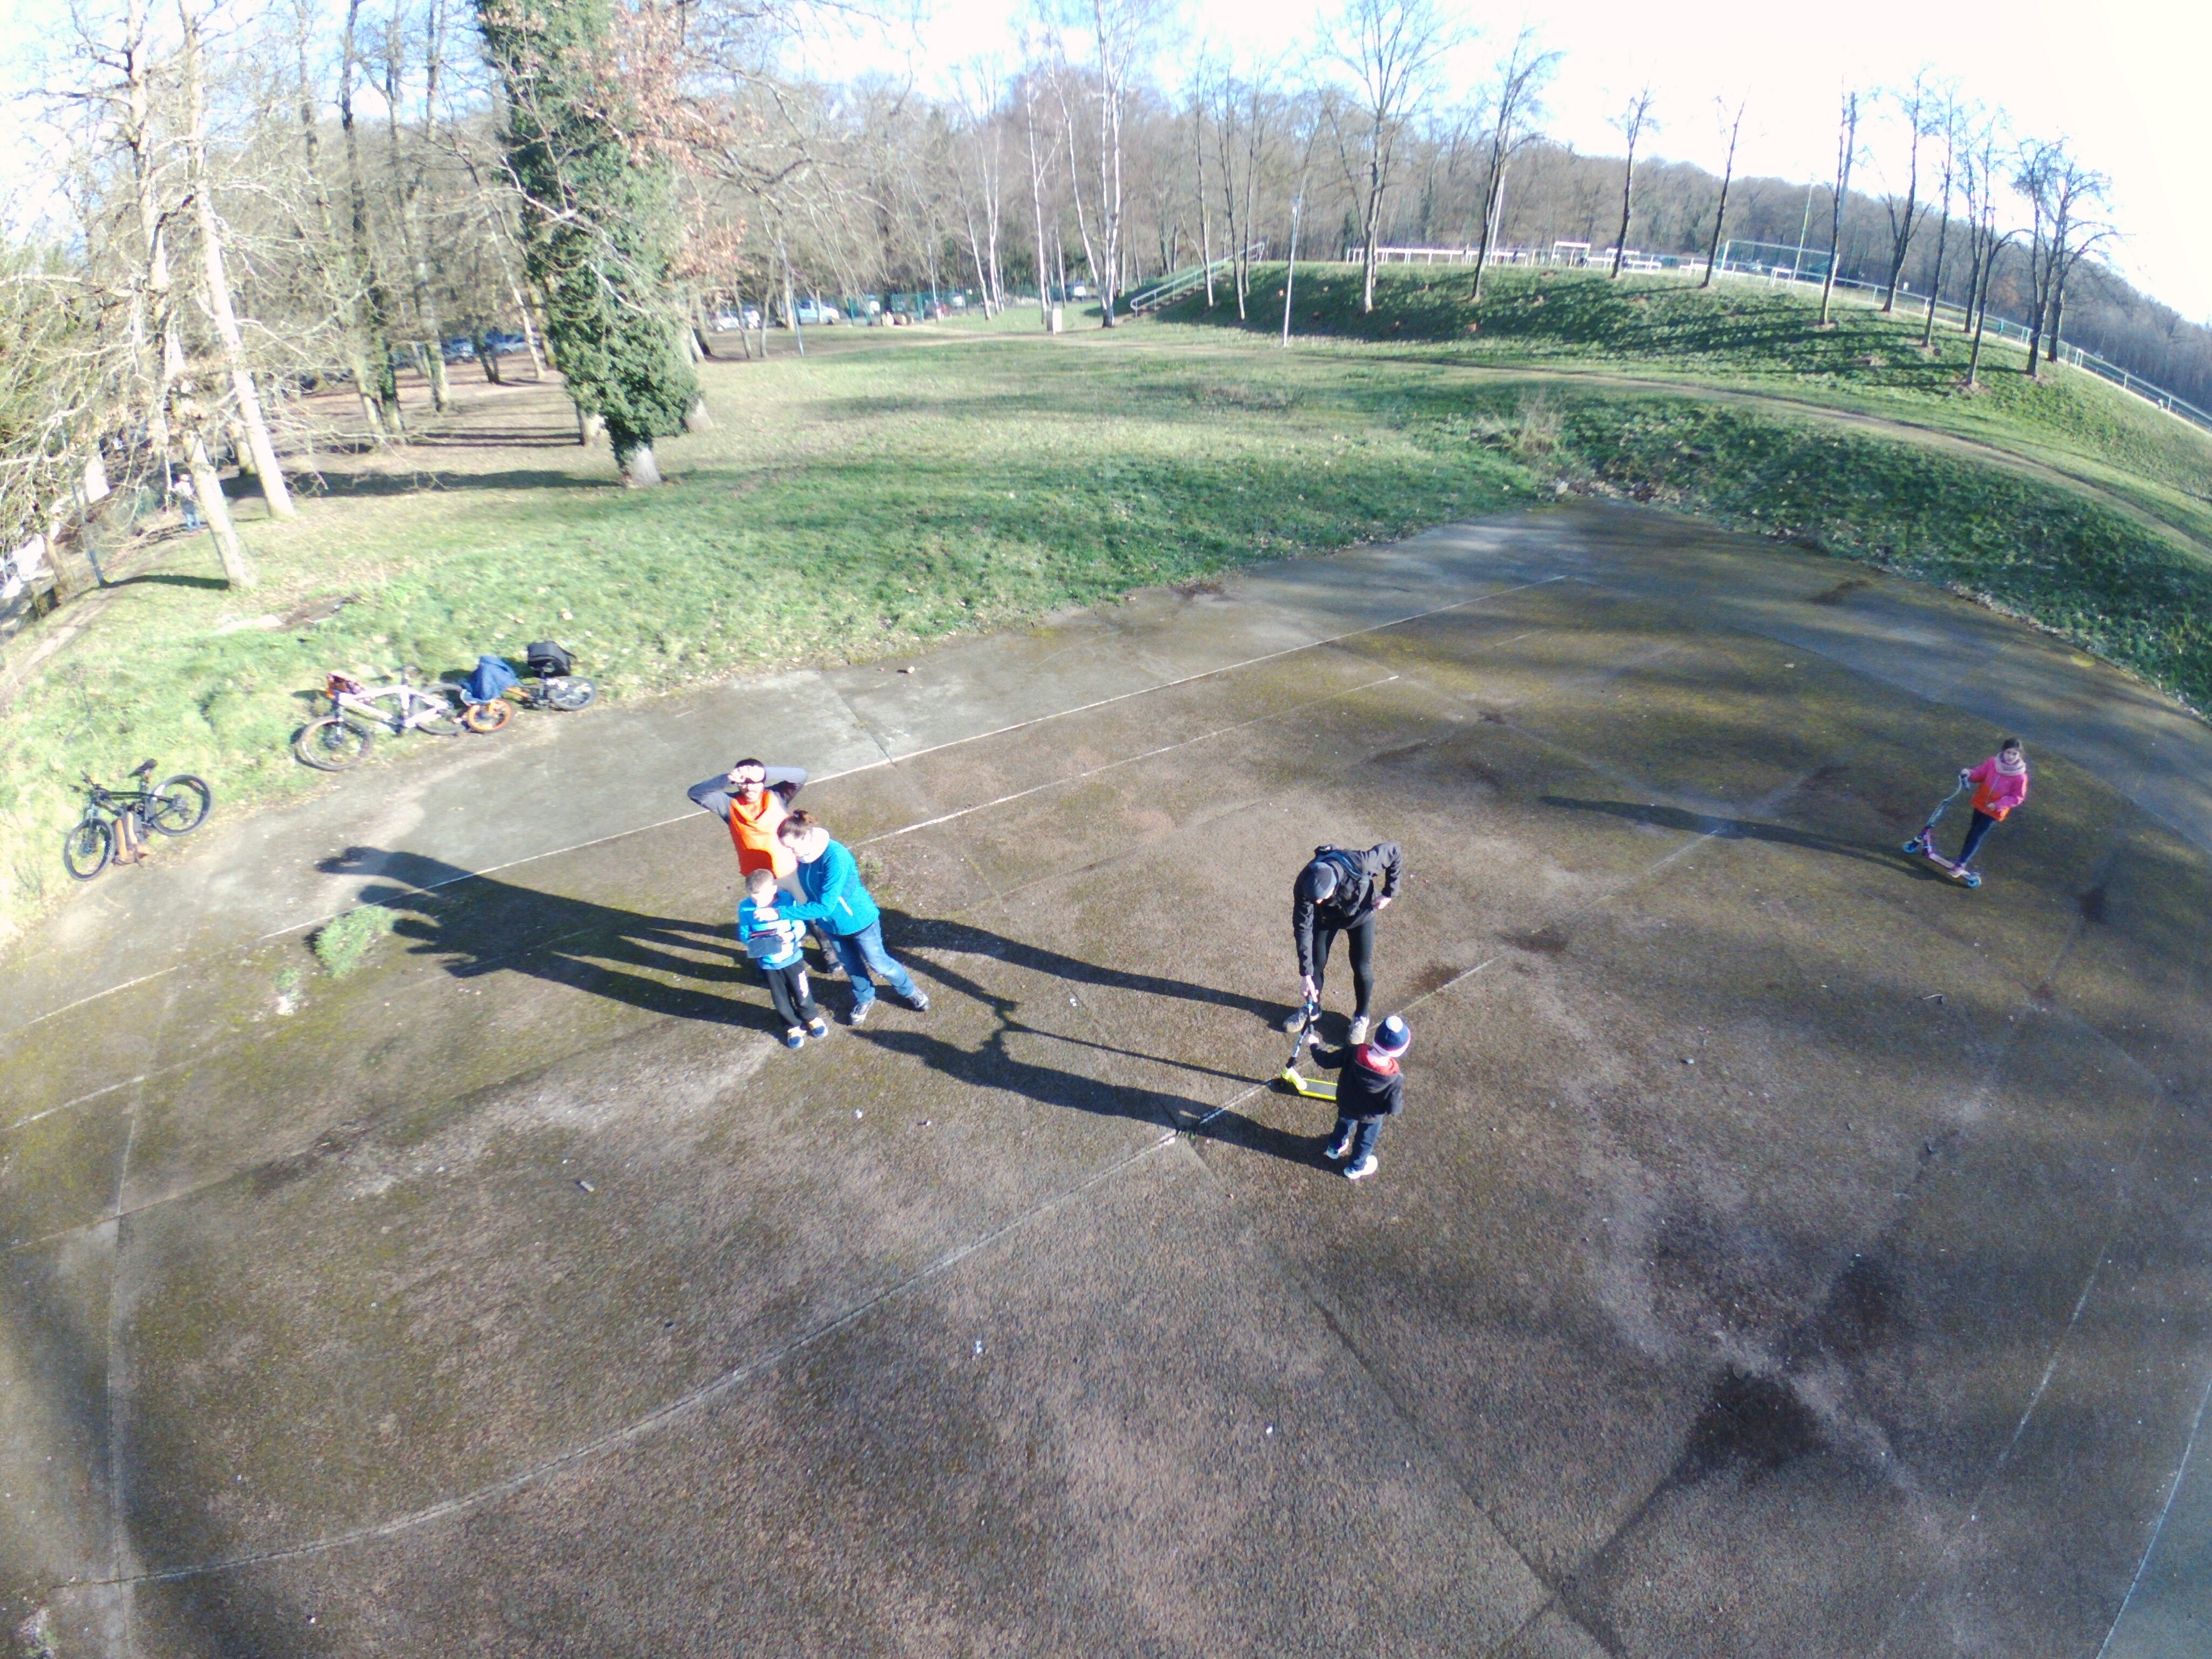
\includegraphics[width=\textwidth]{Bebop_A}}
        \caption{Precence of shadows}
    \end{subfigure}
        ~ %add desired spacing between images, e. g. ~, \quad, \qquad, \hfill etc. 
      %(or a blank line to force the subfigure onto a new line)
    \begin{subfigure}[b]{0.38\textwidth}
        \frame{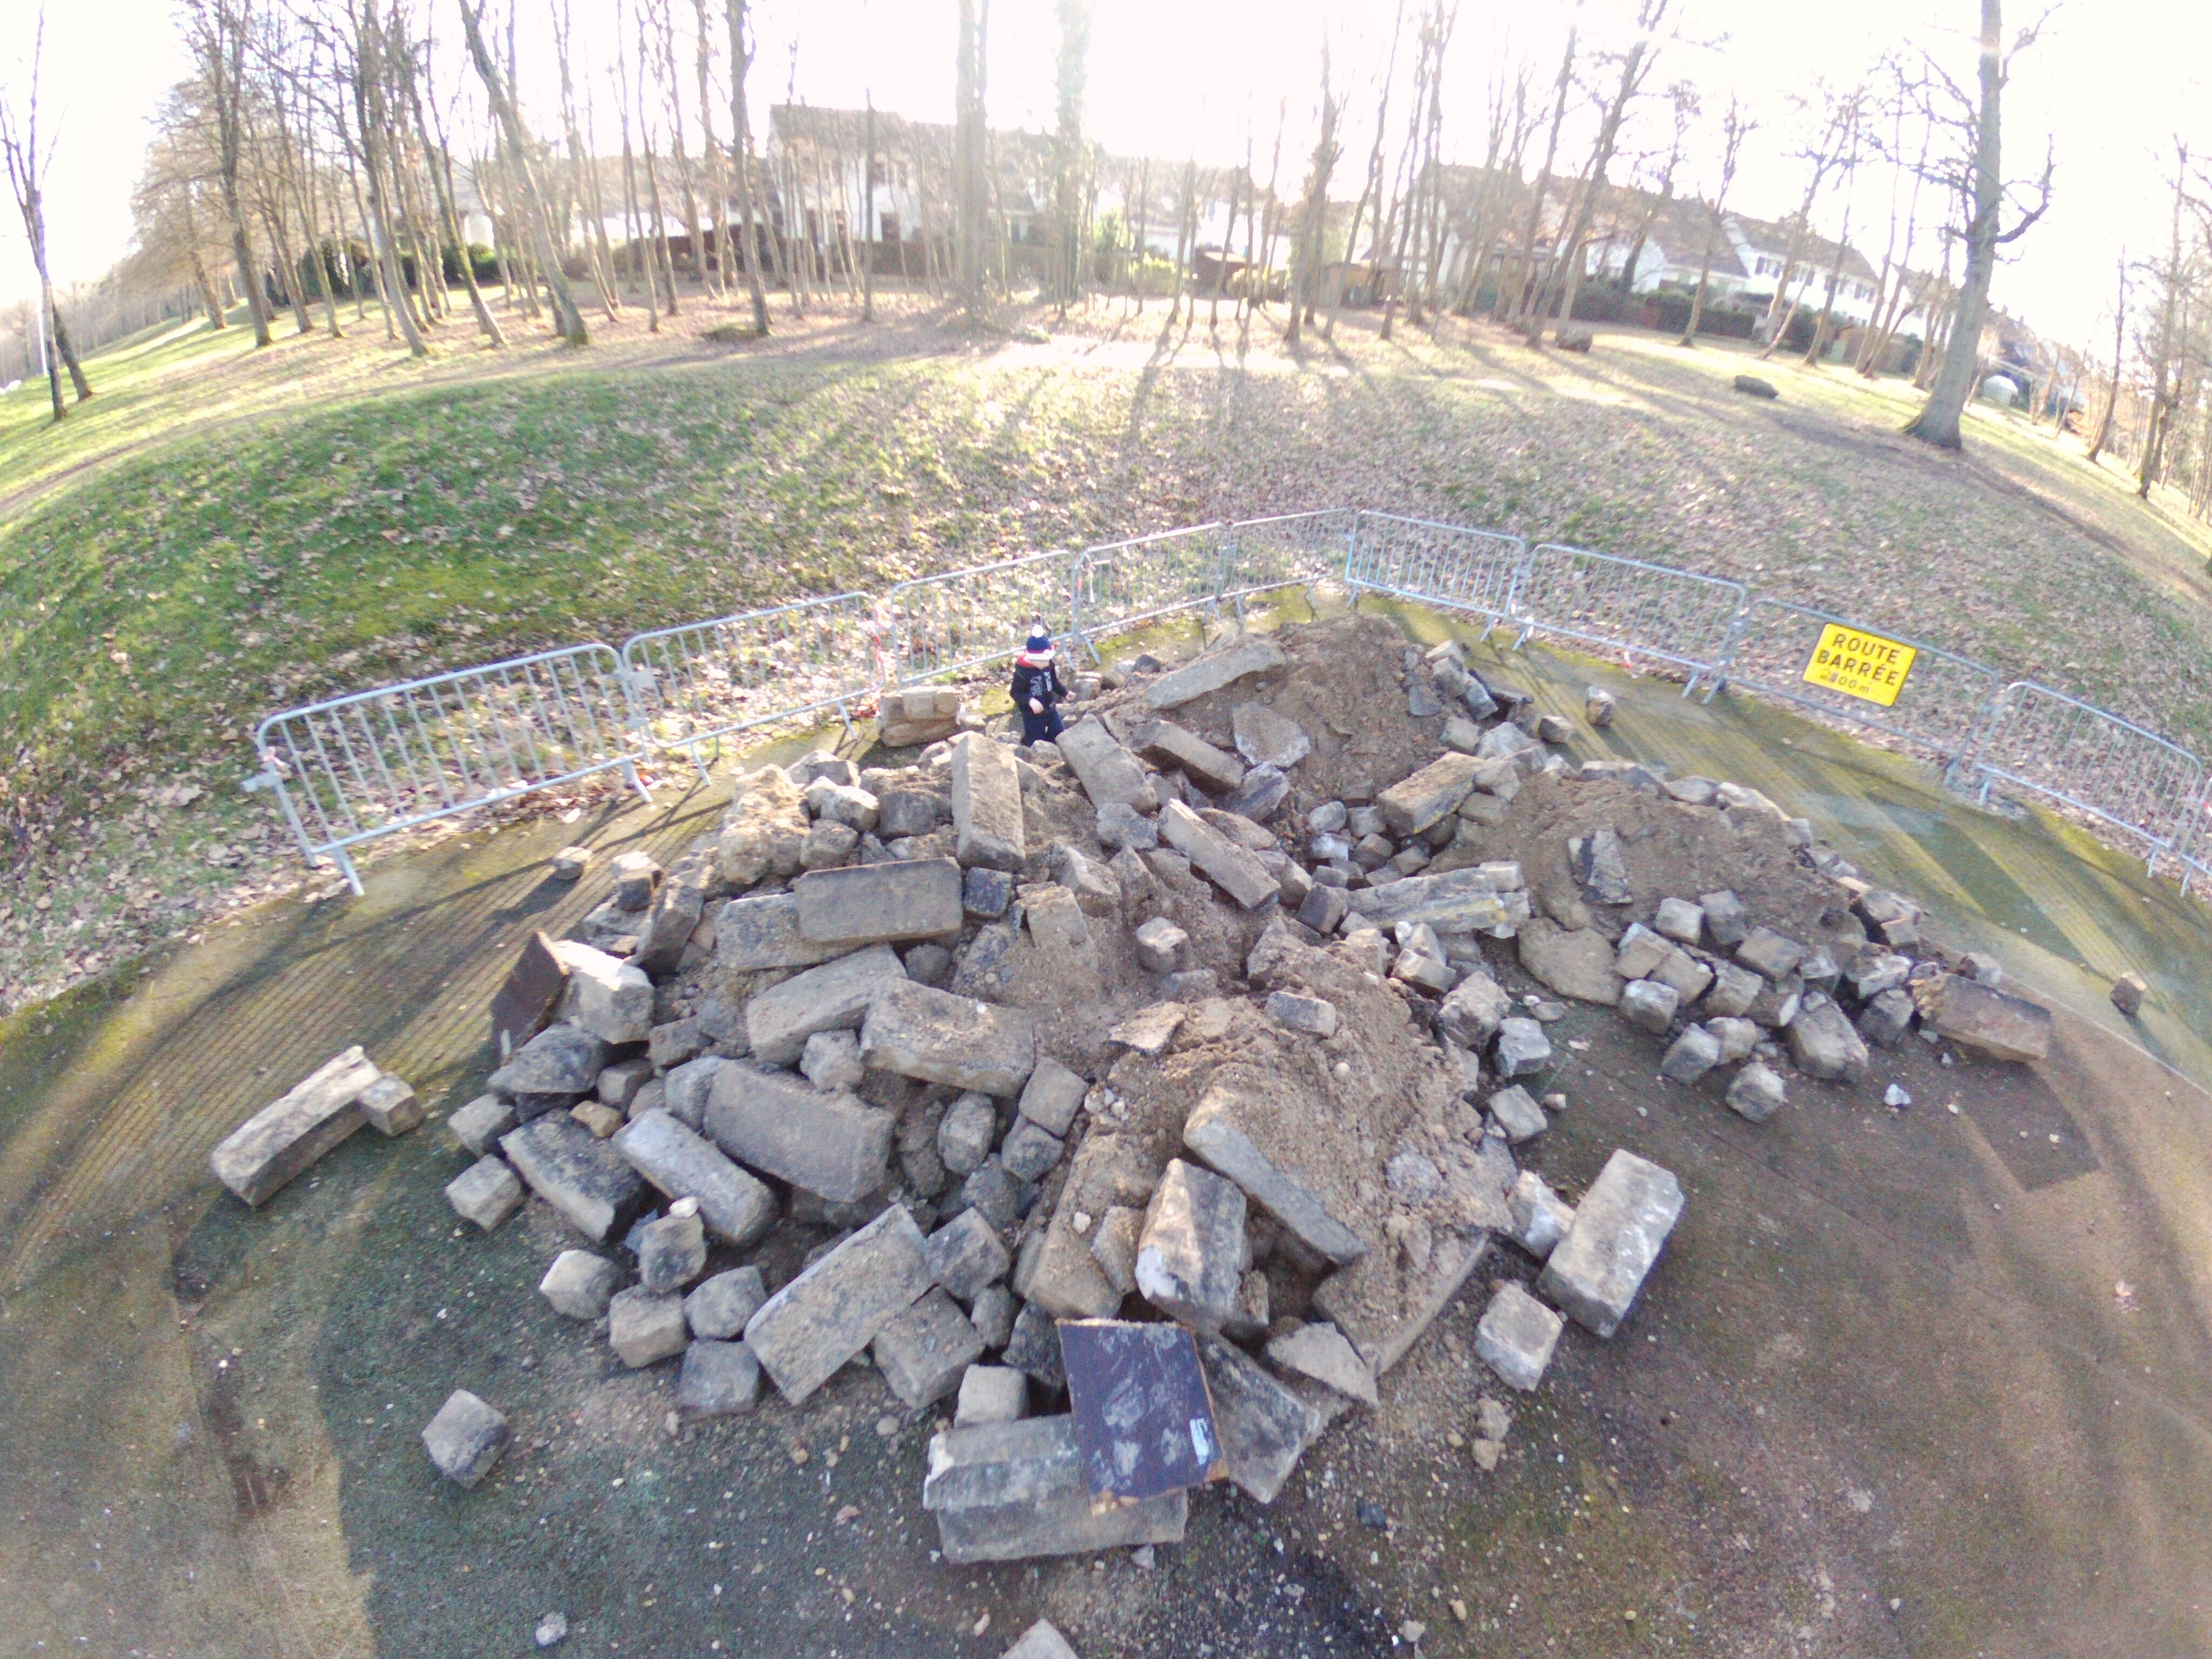
\includegraphics[width=\textwidth]{Bebop_B}}
        \caption{Saturations}
    \end{subfigure}
        ~ %add desired spacing between images, e. g. ~, \quad, \qquad, \hfill etc. 
      %(or a blank line to force the subfigure onto a new line)
    \begin{subfigure}[b]{0.38\textwidth}
        \frame{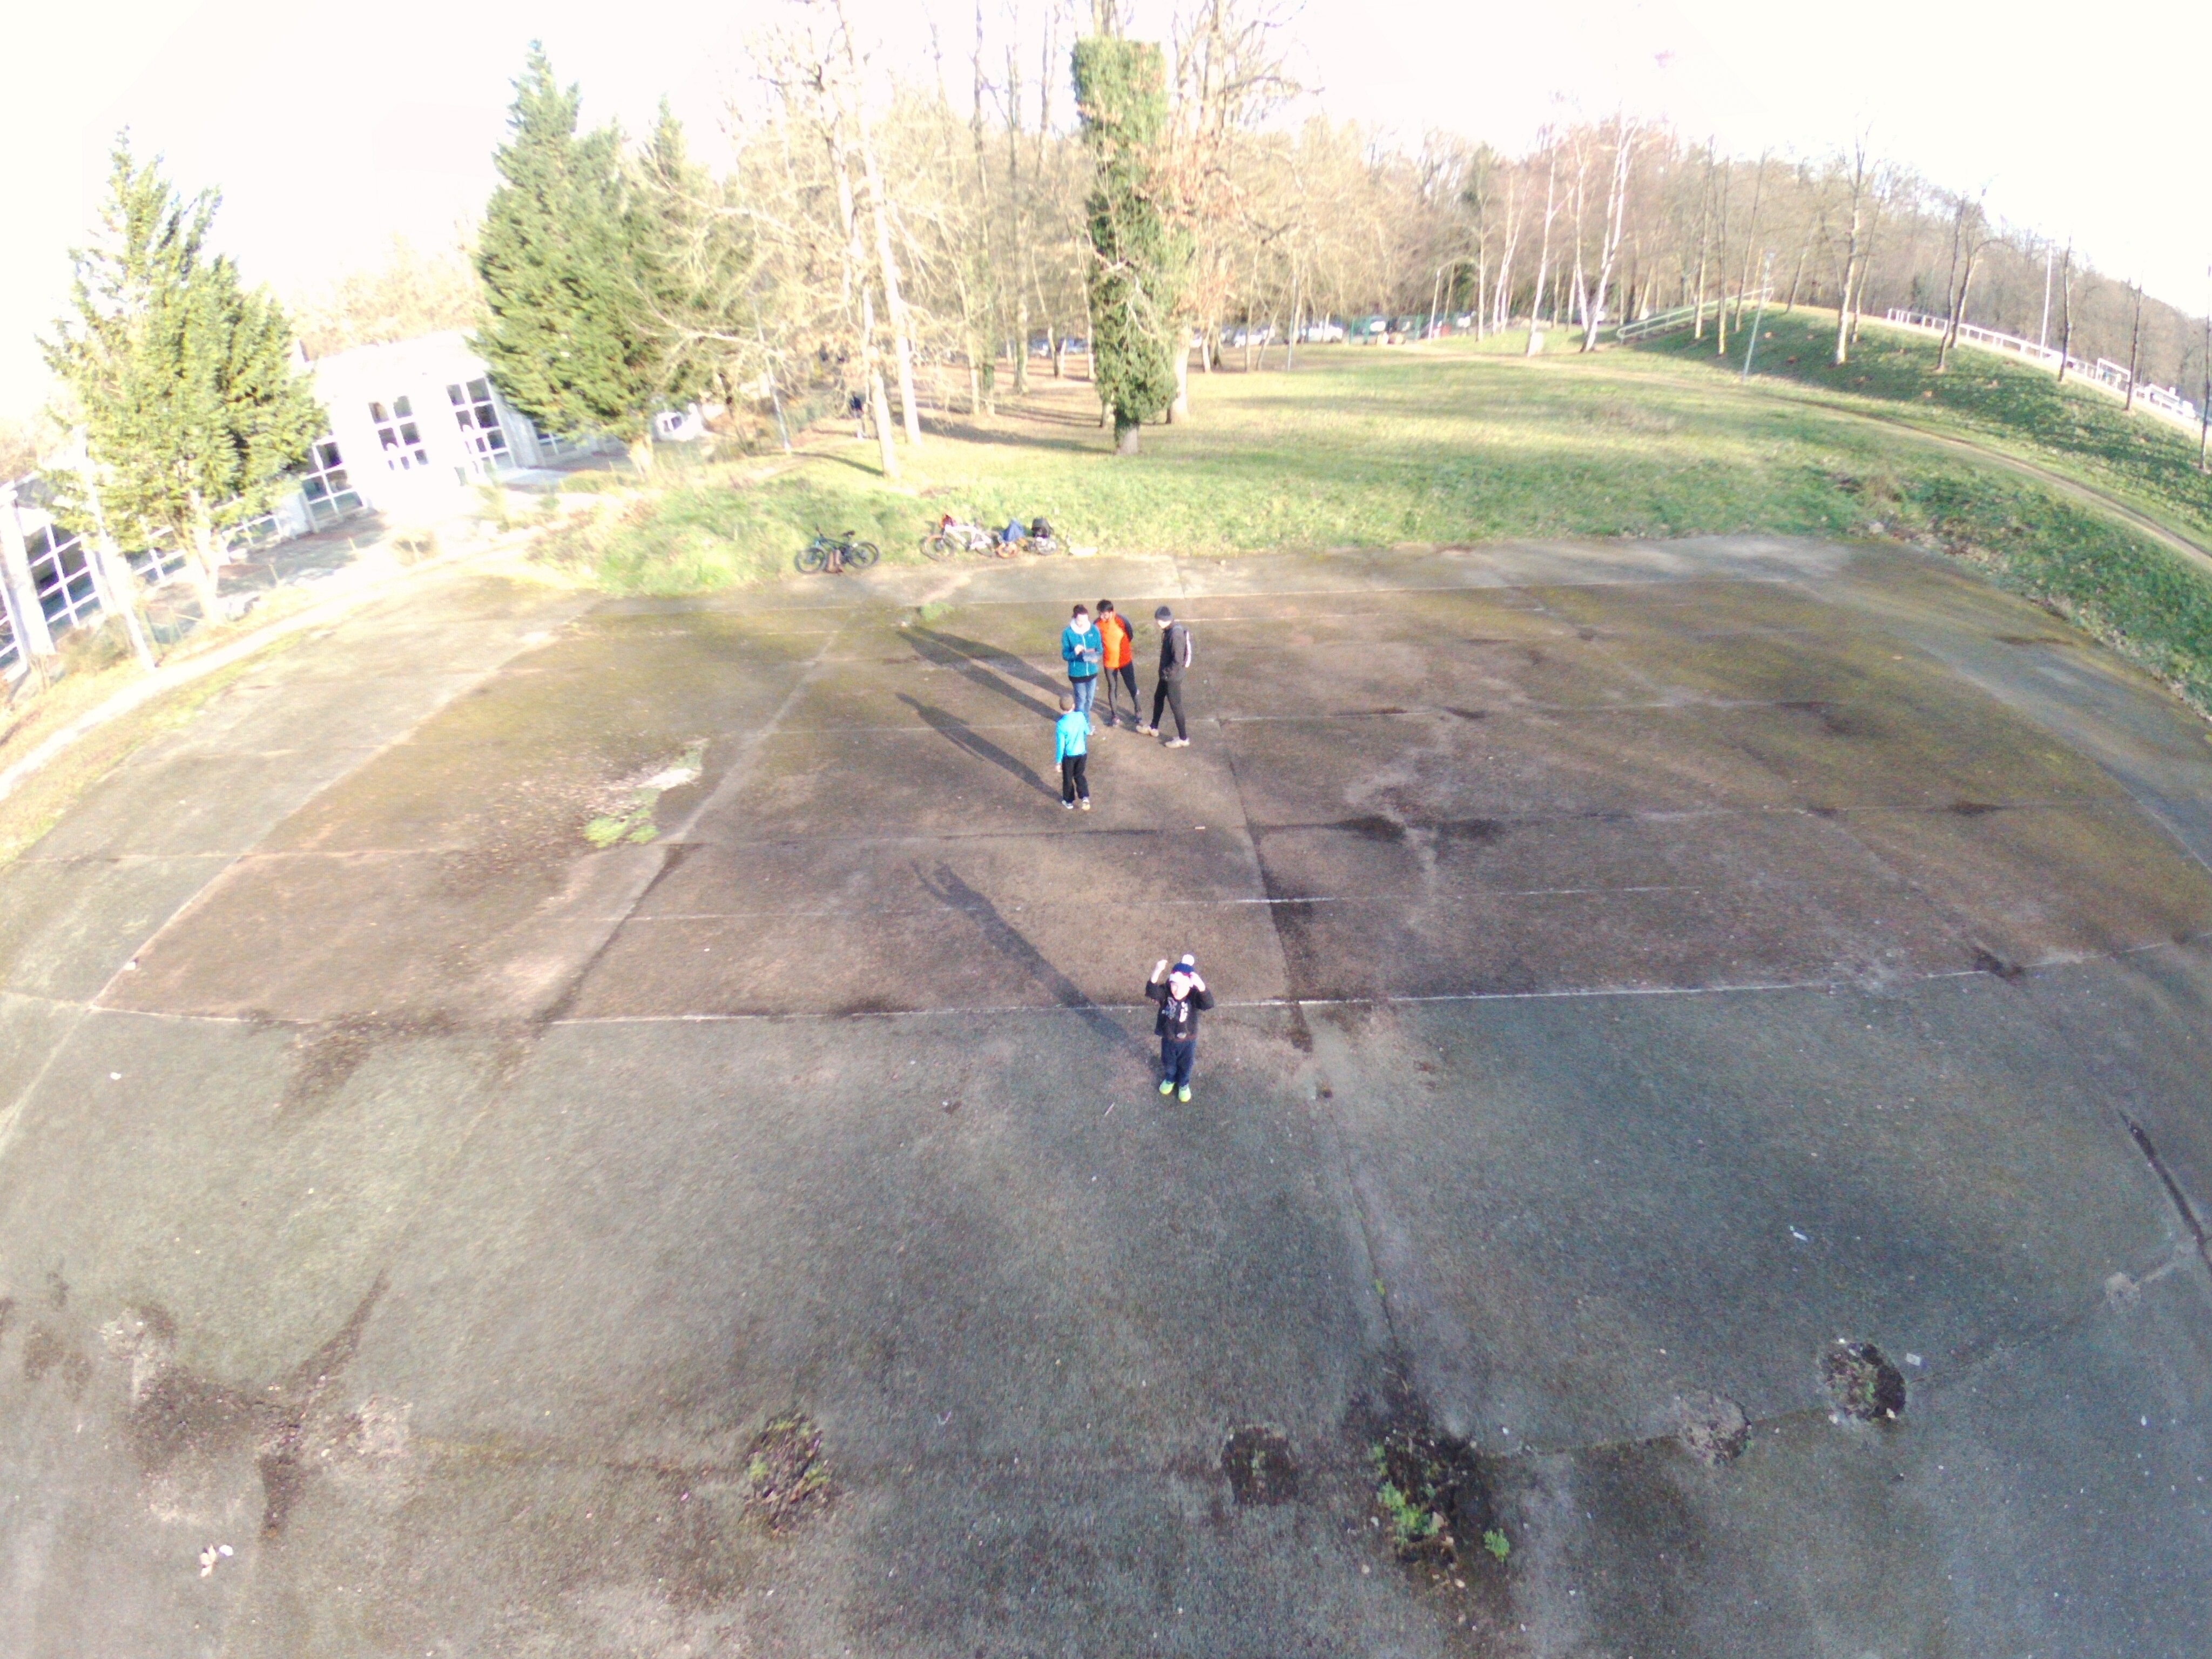
\includegraphics[width=\textwidth]{Bebop_C}}
        \caption{Change of scale}
    \end{subfigure} 
    \caption{Some examples of image degradations present in aerial imaging and UAV applications.}\label{fig:img_drone_degradations}
\end{figure}

In addition to the problems related to the complex scene conditions, we must consider that a drone is subject to sudden changes in the environment, such as wind gusts, which can affect its stability and modify the visual information given by the on-board sensors. In such cases, the vision algorithms for drone navigation must process the input information fast enough to provide answers and transform them into real-time decision actions.

In the literature, we can find a large number of works that deal with drone navigation. Among these works, we can say that the different approaches are strongly related and motivated by the application's aim and the conditions in which it is carried out. However, we can differentiate two main vision-based techniques for UAV navigation; 1) localization and mapping and 2) obstacle avoidance.

Simultaneous Localization and Mapping (SLAM) falls within the first group techniques, where drone navigation is a consistent result. This technique estimates the drone's local pose and builds a 3-d model of its surroundings employing visual sensors.  The Visual Odometry (VO) \citep{Scaramuzza.Fraundorfer:RAM:2011} is responsible for the robot motion estimation while the maps are built with occupancy grid algorithms \citep{Thrun.Bu:AI:1996}. . According to the image information used to perform a SLAM, we can classify these approaches into feature-based methods, which extract a set of image features (e.g., lines, points) in a sequence of images, and direct-based methods, which make use of the image intensity information to estimate the structure and the motion of the robot.

The use of SLAM techniques for UAV navigation presents remarkable advantages. Feature-based methods can use various feature detectors, which typically count with an optimization stage to produce fast algorithms. Direct-based methods have the advantage of being robust to image degradations; they can lead better with images with texture and blurred zones; besides, the map produced is of an acceptable resolution. Interestingly, the strengths of the first group of methods are the weak points of the second and vice versa. A method that tries to gather the benefits of both approaches is the Semi-direct Visual Odometry \citep{Forster.Pizzoli.ea:ICRA:2014}; however, in general, the SLAM methods work in indoor environments, where the illumination conditions are static or controlled.

On the other hand, there are approaches for drone navigation that favor the avoidance of obstacles. This capability is essential for achieving free collision missions in both indoor and outdoor environments. A recurrent solution, as we early mentioned, is the multi-sensor data fusion. \cite{Gageik.Benz.ea:ACCESS:2015} present a platform using low-cost ultrasound and IR sensors; however, despite the obtained results, it utilizes several sensors to retrieve environment information, and yet, it does not get a perceptual representation of the scene due to the low resolution and perceptive capacity of the sensors. On the other hand, vision-based techniques for obstacle avoidance could identify obstacles and, in some cases, classify the found object \citep{Li.Ye.ea:IROS:2016}. 

We can classify the visual methods for avoidance of obstacles into two groups. The first, SLAM-based techniques, make use of the principles above. The 3-d reconstruction provides accurate and sophisticated maps and allows the air vehicle to travel with more information about the environment. In \citep{Moreno-Armendariz.Calvo:ICMEAE:2014}, takes this advantage to develop an obstacle avoidance approach for static and dynamic obstacles.

The second group is the flow-based methods which historically, were inspired by the navigation of insects such as bees \citep{Srinivasan.Gregory:PTBS:1992} or flies \citep{Franceschini.Ruffier.ea:InTech:2009}. Many insects in the wild identify obstacles through the intensity of light. During the flight, their eyes produce an optical flow that provides accurate spatial information. Currently, there are also works inspired by the behavior of the human eye \citep{Al-Kaff.Meng.ea:IVS:2016}. The technique measures the object size from the idea that objects in the robot's vision field are more significant as the obstacle is close.

The techniques for obstacle detection and avoidance present interesting characteristics and ideas. Notwithstanding, its implementation is strongly linked to an application under certain conditions. In consequence, Their use would involve a recalibration or readjustment of parameters. Given the conditions in which a drone can operate, it is necessary to have more general and non-supervised methods.

The most efficient algorithms to date are those based on Neural Network (NN) architectures and supervised learning techniques. Nevertheless, these techniques have remarkable disadvantages that question their usability and applicability in real-life drone missions. From a practical and even economic point of view, there is a limit to the number of applications in which we can use supervised methods given the fact that we need a lot of annotated data. The collection and the correct labeling of data representing a problem are valid only for a small number of applications.

The need for abundant information comes with high computational times required for model learning, ranging from a couple of hours to weeks. Of course, we can minimize this variable by increasing our machines' computing power; however, today, only those with large computing infrastructures can afford to train models with hundreds of billions of parameters.  

The above statement introduces the next disadvantage of deep neural network-based learning models: hyperparameters. We can roughly divide hyperparameters into two categories, 1) optimizer hyperparameters, which include learning rate, batch size, and the number of epochs and 2) model-specific hyperparameters, including the number of hidden layers, the first hidden layer, and the number of layers. Choosing the appropriate hyperparameters plays a crucial role in the success of neural network architectures because they control the learning algorithm's behavior, define the network structure and how the network is trained. Although there are methods to optimize their choice, generally, this task is a heuristic process, and their fine-tuning is a function of the specific application. It is possible to follow some rules based on experience, copy the same values from some other problem or make the setting by trial and error, though we cannot know the best value for a hyperparameter.

\subsection*{Scope of the Thesis}
The interaction between computer vision and applications made with unmanned aerial vehicles is extensive. This collaboration has generated new methodologies and approaches, both theoretical and practical, but has also given way to new research questions. So, we want to detail the scope and focus of this thesis work.

First of all, this thesis work is motivated mainly by my profile and interests in robotics and control theory, specifically in air vehicles. Knowing the fundamental limitations of aerial robots and the complexity of drones' applications, we explore computer vision theory to propose algorithms that improve and provide assistance in drone navigation tasks. In this sense, we are interested in studying the scene's perceptual information for their treatment and interpretation.

We focus primarily on the vision processing problems before the image object recognition: object detection and segmentation. We argue that scene understanding, through object recognition, is a key to UAV navigation, especially when the tasks are developed in complex, uncontrolled environments. From this perspective, we focus on using low-level image features to extract perceptual information. 


Throughout this work, we develop algorithms that use such primitives in conjunction with statistical and geometric tools from computer vision and signal theory. The developed algorithms provide solutions to the recognition and scene understanding problem's variants, such as the classification, identification, and detection of objects from a qualitative point of view, always looking for the application's physical meaning. Instead of using supervised methods, we focus on decomposing the image information from the point of view of signal theory and physics to use it later on non-supervised or mathematical morphology methods. So it is worth mentioning that the practical aspect linked to the implementation and the generation of solutions in real-time are not a priority.

Regarding the nature of the input data, we use only color or black and white images as input information, favoring monocular cameras among the wide range of visual sensors reviewed previously. This choice allows replicating the algorithms with low-cost cameras that can be easily embedded in a drone.

One last point about the focus of this work is about the type of computer vision techniques. The algorithms proposed in this thesis are based on traditional computer vision techniques, that is, non-deep learning techniques. This decision is consistent with drone applications' nature, where there are not necessarily rich enough annotated databases to apply the most sophisticated artificial intelligence models.

\section*{Objectives of the Thesis}\label{sec:objectives_of_the_thesis}

In this Ph.D. thesis, we aim to develop general computer vision algorithms considering the challenges and needs of UAV navigation. In this context, the primary objective is to propose a new methodological framework for decomposing images prior to detecting objects and understanding scenes. As we mentioned before, the idea is to apply this framework to assist in control and decision-making in drone navigation tasks. Therefore, the framework must be robust to image degradations existing in environments with uncontrolled conditions, in addition to being independent of the choice of specific parameters for its operation.

During the thesis, we consider many specific drone tasks, such as:

\begin{enumerate}[label=\roman*]
	\item \textbf{Recognition} is a classic computer vision problem responsible for determining whether an image contains an object, characteristic, or exercise. Some variants of this problem are the classification, identification, and detection of objects from which many specialized tasks emerge. For example, content-based image search, pose estimation, optical character recognition, reading of 2-d codes, facial recognition, shape recognition, among others.
	\item Environment awareness.
	\item Detection and avoidance of obstacles.
	\item Identification and following of targets.
\end{enumerate}
Given these tasks, the work focuses on the scene understanding problem. To deal with this problem, we deepen the study of low-level image primitives such as contours, color, texture, and texture color. Therefore, some secondary objectives involve building a representative feature space using concepts from signal theory, geometry, and statistics, in addition to concepts from human perception.

The idea is to gather these features under an unsupervised framework without specific parameters, using traditional machine learning and segmentation algorithms. Figure \ref{fig:general_diagram_framework} a general diagram of the framework we propose. The first stage of the framework consists of extracting the primitives from the image, here we work with contours, color, texture, and the relationship between color and texture. The second block of the framework exploits the perceptual information contained in the extracted primitives. Finally, the framework's third block applies different methods (supervised or unsupervised) to the image's feature space to solve various computer vision problems.  Although the framework itself is an ambitious goal, in this thesis, we present several algorithms that apply the framework methodology with one or more features to solve different computer vision problems such as object detection and recognition, image retrieval systems, perceptual object boundaries detection, and image segmentation.

The interest of obtaining a representative space of the image information from low-level hand-made features lies in the possibility of using it in a semi-supervised pipeline. By injecting annotated information into the frame, it might make generalizations and obtain medium- or high-level features such as the importance of color and texture information to a human when segmenting an image.

\begin{figure}[!ht]
    \centering
    \includegraphics[width=\textwidth]{general_framework_diagram}        
    \caption{Proposed framework for object detection and scene understanding.}\label{fig:general_diagram_framework}
\end{figure}

Several secondary objectives are present throughout the study of each of the low-level primitives and their resulting features.

\begin{itemize}
	\item \textbf{Framework implementation.} This objective refers to the first stage of implementation in simulated and off-board environments. In a second moment, to the implementation in a real platform. The latter requires the search for a portable platform capable of real-time operation.
 
	\item \textbf{Framework functional evaluation.} Comparison of the obtained results regarding the approaches of state of the art.
 
 	\item \textbf{Framework validation.} Real test deployment taking into account the constraints of portability and real-time on the industrial scale.
 
\end{itemize}

Finally, this thesis aims to show that traditional computer vision methods are (still) a reliable option to develop object detection and recognition for relatively complex tasks. Especially in the current context of computer vision, where there are hundreds of algorithms based on neural networks and artificial intelligence for image segmentation and object detection that are highly performant but lack a physical (and in many cases logical and argued) interpretation of its results. Furthermore, these algorithms are in trouble when it comes to image analysis of complex scenarios or applications where there is no database rich enough to do the learning process.


\section*{Organization of the Document}
We explore three low-level primitives during this thesis; contours, color, and texture. The organization of this document follows, to some extent, the evolution of the construction of the vision-based framework for object detection and aid in drone navigation. This thesis will then be decomposed into two parts:

\begin{enumerate}
	\item A part dedicated to studying the contours of the image, in which we review in detail some of the classic methods for obtaining image contours. We use this information in conjunction with the \textit{a contrario} method and the Gestalt organizing laws to detect and identify landing targets.
	\item The second part main topic is the study of the properties of color and texture of an image. In the first moment, we are interested in the global distribution of this information and the existing metrics to measure the similarity between the distributions; we apply and validate these concepts in a retrieval image system. Subsequently, we extend the study of color and texture in images, exploding the local distribution of these primitives and studying the influence of color information on the generation of textures in an image. We propose a completely unsupervised framework for the detection of perceptual boundaries. Furthermore, we explore different strategies to obtain the segmentation of natural images using the obtained perceptual boundaries.
\end{enumerate}

More specifically, the chapters contained in the three sections are structured as follows:

\begin{itemize}
	\item \textbf{Chapter \ref{ch:landing_target_detection}} addresses the bases of the Gestalt theory, including the grouping laws and the Helmholtz principle. We formalize these concepts of human perception mathematically and formulate a non-parametric algorithm that follows an unsupervised framework based on an image's contours. We use the developed framework in the autonomous drone landing problem, specifically detecting and identifying landing targets.  The chapter also presents a review and a quantitative comparison of different traditional methods for extracting image contours.
	
	\item \textbf{Chapter \ref{ch:color_texure_representations}} presents a detailed review of the different ways to represent the color and texture information in an image. The chapter contains a review of various color spaces and their main properties and an introduction to the different techniques for characterizing textures in the literature. Such information is of relevant importance in the construction of the framework and the approaches to measure similarity between distributions.
	
	\item \textbf{Chapter \ref{ch:similarity_measures}} presents the analysis between different similarity measures between distributions, showing the advantages and disadvantages of each of them. In particular, we focus on the theory of optimal transport through the Earth Mover's Distance. We show the advantages of this metric over traditional similarity measures using an image retrieval system based on an image's global color and texture information.
	
	\item \textbf{Chapter \ref{ch:spectral_image_decomposition}} delves into the physical and human perception aspects of Gabor's filters. We show the steps involved in designing an optimized and efficient Gabor family of filters. The proposed filter family models and captures the texture information through an energy-efficient decomposition of the image. Such spectral decomposition of the image deals with Heisenberg's uncertainty principle. The chapter presents the description of parameters that allow complete customization of the filter family according to the application.
	
	\item \textbf{Chapter \ref{ch:complex_spectral_image_decomposition}} brings an analysis of the texture information present in color images, showing the strong relationship between those two features. Using the spectral analysis of an image with the previously defined Gabor filters, we generate a feature space that simultaneously captures the color and texture information. We show the richness of such feature space by performing unsupervised image segmentation only using simple clustering techniques.
	
	\item \textbf{Chapter \ref{ch:perceptual_object_boundaries_detection}} introduces a framework for the detection of perceptual boundaries of objects present in natural images. This framework brings together concepts addressed in this document, such as the spectral decomposition of images, the optimal transport as a true metric, and the relationship between color and texture information. Besides, using the hierarchical segmentation technique, we segment natural images in an unsupervised manner. We perform a quantitative and qualitative validation of our method using a known database.
	
	\item \textbf{Chapter \ref{ch:general_conclusion}} contains the general conclusions of the thesis and addresses the different possible research lines as a continuation of this work.
	
\end{itemize}
%    \afterpage{\blankpage}
	\cleardoublepage

%	% created on 28/07/2020
% @author : ebazan
\part{Global Color and Texture}\label{part:global_color_texture}%Image Global Color and Texture

\section*{Introduction}
In part \ref{part:image_contours}, we show that low-level features, such as image contours, provide useful perceptual information that can be used to solve complex problems. We presented a framework that uses the concepts of human perception and contour information for the unsupervised detection of landing targets. This framework is able to identify the marker under degraded operating conditions using only exogenous features from the contours, which are identified on gray-level images. The framework can be improved by adding other features that provide perceptual information of a scene.

In this part of the thesis, we review two more low-level image features: color and texture. Both features are widely involved in the perceptual process of humans and their study can be very extensive. The objective of this part is to explore the image color and texture features for their future integration into a general framework for object detection. Particularly, in this part of the thesis we are interested in the global distribution of color and texture information of an image. For this purpose, the chapter that opens this part seeks to remember recall the definition of color and texture in the field of computer vision. Moreover, it review different approaches to color representation as well as different strategies for characterizing texture features. Later, in chapter \ref{ch:similarity_measures}, we take interest at the comparison of distributions, particularly in the study of the Optimal Transport (OT) as a metric for the measurement of similarity between distributions and its application in the field of computer vision.

Throughout these chapters of the thesis, we address the study of those two properties using simple images containing the information of interest; in the case of color, images containing low color variation and; in the case of texture, grayscale images with homogeneous textures.

The main contributions of this part are:

\begin{enumerate}
	\item Review of the state of the art of global color representations and texture characterizations.
	\item Review of the state of the art of similarity measures, particulary the interpretation of the OT in computer vision: the Earth Mover's Distance (EMD).
	\item Qualitative and quantitative study between the most popular measures in the comparison of distributions and the EMD. 
	\item An unsupervised image retrieval system based on global color/texture information.
\end{enumerate}


\chapter{Global Representations of Color and Texture } \label{ch:color_texure_representations}

\section*{Résumé}
\noindent 
Ce chapitre présente une compilation des différentes manières de représenter les informations de couleur et de texture présentes dans une image. En ce qui concerne les informations de couleur, nous introduisons certains types d'espaces colorimétriques et leurs origines. De plus, nous présentons quelques techniques pour synthétiser ces informations. Dans le cas de la texture, nous présentons les différentes méthodologies pour son étude, en mettant en évidence les avantages et les inconvénients de chaque méthode.
\section*{Abstract}
\noindent 
This chapter presents a compilation of the different ways of representing the color and texture information present in an image. When it comes to color information, we present some of the most popular color spaces used as well as their origins and relationship to human perception. In addition, we present some techniques to synthesize this information. In the case of texture, we present the different methodologies for its study, highlighting the advantages and disadvantages of each method. The information presented in this chapter serves as the basis for the next chapter.

\section{Introduction}

If we look around us, we can see that many of the materials and objects of our environment only exist with certain colors. For example, the clouds are mostly  white, the grass is green, the ocean is blue, etc. Performing the same experience, but this time with textures, we realize that we are surrounded by them everywhere. We find textures, for example, at textiles, buildings, tilings and on skins or objects surfaces. The color and texture of an image is very valuable information and therefore, the perception of such information is a powerful tool for classifying and recognizing certain objects and materials.

For decades several vision algorithms have sought to exploit this information. Color and texture are of relevant importance for its use as a feature to characterize objects. Due to these facts, the definition and the various representations of the color, as well as the texture information, is addressed in this chapter. As far as color information is concerned, we give a brief introduction to what color is and how it can be represented. In the case of texture, we present a brief introduction to textures including its types and an overview to the various methodologies for its study, highlighting the advantages and disadvantages of each method. 


\begin{figure}[!ht]
    \centering
    \begin{subfigure}[b]{0.24\textwidth}
        \includegraphics[width=\textwidth]{tempo}
        \caption{}
        \label{fig:tempo}
    \end{subfigure}
    %~ %add desired spacing between images, e. g. ~, \quad, \qquad, \hfill etc. 
      %(or a blank line to force the subfigure onto a new line)
    \begin{subfigure}[b]{0.24\textwidth}
        \includegraphics[width=\textwidth]{mountain}
        \caption{}
        \label{fig:parrots}
    \end{subfigure} 
    %~ %add desired spacing between images, e. g. ~, \quad, \qquad, \hfill etc. 
      %(or a blank line to force the subfigure onto a new line)    
    \begin{subfigure}[b]{0.24\textwidth}
        \includegraphics[width=\textwidth]{clownfish}
        \caption{}
        \label{fig:clownfish}
    \end{subfigure}
    %~ %add desired spacing between images, e. g. ~, \quad, \qquad, \hfill etc. 
      %(or a blank line to force the subfigure onto a new line)
    \begin{subfigure}[b]{0.24\textwidth}
        \includegraphics[width=\textwidth]{araras}
        \caption{}
        \label{fig:mountains}
    \end{subfigure}
                  
    \caption{Some examples of color images: One synthetic image {\small \textsf{\textbf{(a)}}} and three natural images [{\small \textsf{\textbf{(b) (c) (d)}}}].}\label{fig:color_images}    
\end{figure}


\section{Color}

Color is a physical property linked to the electromagnetic spectrum of light \citep{Beyerer.Leon.ea:Book:2016}. The perception of color in humans results from the quantity and wavelength captured by the eyes. This perception depends on many factors such as the type of surfaces or objects where the light is reflected, the environment and even the eyes of the observer. The perception of color is then an entirely arbitrary creation of our nervous system, and there is no way it is contained in the wavelengths or in light-reflecting objects and materials \citep{Goldstein:Book:2009} \citep{Beyerer.Leon.ea:Book:2016}. When an incident spectrum contains all frequencies in the range of visible wavelengths, humans perceive objects that reflect all frequencies as clear or \textit{white}. In the opposite case, when the material absorbs and does not reflect the visible frequencies, it is perceived as dark or \textit{black} {Gonzalez.Woods:Book:2008}. 

Although color has measurable physical properties, the interpretation and perception of this information is completely subjective. A clear example of this is the naming of colors. Some works in this regard state that the naming of colors varies according to culture and language \citep{Berlin.Kay:Book:1991}. However, it is possible to find a correlation between languages and identify eleven basic color terms in English language that  seem to be anchored across the different languages as points in a certain color space \citep{Kay.Regier:PNAS:2003}. The definition of a coherent color space to the final task is therefore essential to represent the color information digitally.


\section{Color representation}

The representation of color has evolved over time developing theories, such as the trichromatic theory or the opponent-colors theory \citep{Fairchild:Book:2005}, that attempt to explain the function of color vision. The result of these theories has been the development of abstract mathematical models that serve to represent colors as vectors or tuples of numbers. These vectors, which are mostly in three dimensions, can be arranged in a variety of ways. Such particular organizations are known as color models.

One of the main contributors in the creation of color spaces is the \textit{Commission Internationale de l'Éclairage} (CIE) \citep{CIE:Journal:1932}, who defined the three standard primaries of color $X$, $Y$ and $Z$. These primaries allow to define any visible color of the spectrum (see figure \ref{fig:visual_spectrum}) as a weighted sum of the three primary colors. They are defined mathematically with positive color-matching functions that specify the amount of each primary needed to describe any spectral color \citep{Wright:BookCh2:2007}. This color model is known as the CIE 1931 XYZ.

The \textbf{XYZ color model} quantify an object’s color using a standardized method taking into account the human eye’s (observer) response to these colors in the calculation. $X$, $Y$ and $Z$ are the amount of each primary needed to produce a desired color
\begin{eqnarray} 
 C(\lambda) = (X,Y,Z) \label{eq:g_energy}
\end{eqnarray}
where the primary $Y$ is chosen such that its colour-matching function exactly matches the luminous-efficiency function for the human eye \citep{Wright:BookCh2:2007}. Therefore, to define a color in this space, we need to provide the weights fot the $X$, $Y$ and $Z$ primaries, for example, color $=xX + yY + zZ$. 
 

\begin{figure}[!ht]
    \centering
    \begin{subfigure}[b]{0.45\textwidth}
        \includegraphics[width=\textwidth]{CIE_visible_spectrum}
        \caption{}
        \label{fig:visual_spectrum}
    \end{subfigure}
    %~ %add desired spacing between images, e. g. ~, \quad, \qquad, \hfill etc. 
      %(or a blank line to force the subfigure onto a new line)
    \begin{subfigure}[b]{0.45\textwidth}
        \includegraphics[width=\textwidth]{CIE_chromaticity_diagram}
        \caption{}
        \label{fig:chrom_diagram}
    \end{subfigure} 
                      
    \caption{CIE 1931 2 Degree Standard Observer: visible light spectrum {\small \textsf{\textbf{(a)}}} and chromaticity diagram {\small \textsf{\textbf{(b)}}}.}\label{fig:cie_standard_observer}    
\end{figure}


The \textbf{RGB color model} According to the three-component theory, our eyes only respond three primary colors of light; red, green, and blue . This theory gave rise to one of the first color models, which says that nearly all colors in the visible spectrum could be generated from the mixture of these three primaries (e.g. combining red and green produces yellow)\citep{Goldstein:Book:2009}. This occurs mainly because the red, green, and blue primaries of this color model are not standarized. 







\textbf{HSV color model}

\textbf{HSL color model}

\textbf{LAB color model} (also known as CIEL*a*b* or CIELAB)


\begin{itemize}

	\item \textbf{RBG (Red-Green-Blue)} A color space that maps the amount of red, green and blue light perceived to reproduce the visible color gamut.
	\item \textbf{HSV (Hue-Saturation-Value) and HSL (Hue-Saturation-Lightness)} Alternative representations to the RGB color space that more closely aligns with the way human vision perceives color-creating attributes.
	\item \textbf{Lab (CIEL*a*b*) / Luv (CIEL*u*v*).} A color space where L compenent represents luminance and a* and b* (resp. u* v*) components represent chroma. This representation was created to reflect the high sensitivity of humans to changes in luminance in the perception of color.
\end{itemize}


\begin{figure}[!ht]
    \begin{subfigure}[t]{\dimexpr0.3\textwidth+20pt\relax}
    	\makebox[20pt]{\raisebox{35pt}{ \rotatebox[origin=c]{90} {\small \textsf{\textbf{Input image}}} }}%
    	\includegraphics[width=\dimexpr\linewidth-20pt\relax]{araras}
    \end{subfigure} \\    
     
    \begin{subfigure}[t]{\dimexpr0.3\textwidth+20pt\relax}
    	\makebox[20pt]{\raisebox{35pt}{ \rotatebox[origin=c]{90} {\small \textsf{\textbf{RGB channels}}} }}%
    	\includegraphics[width=\dimexpr\linewidth-20pt\relax]{araras_R}
    \end{subfigure}      
    ~ %add desired spacing between images, e. g. ~, \quad, \qquad, \hfill etc. 
      %(or a blank line to force the subfigure onto a new line)
    \begin{subfigure}[b]{0.3\textwidth}
        \includegraphics[width=\textwidth]{araras_G}
    \end{subfigure}
    ~ %add desired spacing between images, e. g. ~, \quad, \qquad, \hfill etc. 
      %(or a blank line to force the subfigure onto a new line)
    \begin{subfigure}[b]{0.3\textwidth}
        \includegraphics[width=\textwidth]{araras_B}
    \end{subfigure} \vspace{5pt}      
    
    \begin{subfigure}[t]{\dimexpr0.3\textwidth+20pt\relax}
    	\makebox[20pt]{\raisebox{35pt}{ \rotatebox[origin=c]{90} {\small \textsf{\textbf{HSV channels}}} }}%
    	\includegraphics[width=\dimexpr\linewidth-20pt\relax]{araras_H}
    \end{subfigure}     
    ~ %add desired spacing between images, e. g. ~, \quad, \qquad, \hfill etc. 
      %(or a blank line to force the subfigure onto a new line)
    \begin{subfigure}[b]{0.3\textwidth}
        \includegraphics[width=\textwidth]{araras_S}
    \end{subfigure}
    ~ %add desired spacing between images, e. g. ~, \quad, \qquad, \hfill etc. 
      %(or a blank line to force the subfigure onto a new line)
    \begin{subfigure}[b]{0.3\textwidth}
        \includegraphics[width=\textwidth]{araras_V}
    \end{subfigure} \vspace{5pt}  
        
    \begin{subfigure}[t]{\dimexpr0.3\textwidth+20pt\relax}
    	\makebox[20pt]{\raisebox{35pt}{ \rotatebox[origin=c]{90} {\small \textsf{\textbf{LAB channels}}} }}%
    	\includegraphics[width=\dimexpr\linewidth-20pt\relax]{araras_L}
    \end{subfigure}    
    ~ %add desired spacing between images, e. g. ~, \quad, \qquad, \hfill etc. 
      %(or a blank line to force the subfigure onto a new line)
    \begin{subfigure}[b]{0.3\textwidth}
        \includegraphics[width=\textwidth]{araras_a}
    \end{subfigure}
    ~ %add desired spacing between images, e. g. ~, \quad, \qquad, \hfill etc. 
      %(or a blank line to force the subfigure onto a new line)
    \begin{subfigure}[b]{0.3\textwidth}
        \includegraphics[width=\textwidth]{araras_b}
    \end{subfigure} 

	\caption{Color channels of an image in different color spaces in a grayscale}\label{fig:images_color_space}    
\end{figure}

The overall distribution of color within an image is a useful clue that contributes to the description of the content of an image. For example, we can characterize images that contain landscapes with mountains, jungles, urban environments, deserts or other scenes with different elements by their color distribution. The global color distribution can be represented by means of a color image histogram, which is a discrete function that associates to each intensity value (per color channel) the number of pixels that belong to this value.

The advantages of this representation is that they are invariant to the rotation or translation of the image, as well as, to a lesser extent, to changes of point of view and changes of scale. In addition, we can compact the image color information by reducing the count intervals, that is, by selecting a small number of bins.

\subsection{Single-channel Color Histogram}

\begin{figure}[!ht]
    \centering
    \begin{subfigure}[b]{0.45\textwidth}
        \includegraphics[width=\textwidth]{araras}
        \caption{Input image}
    \end{subfigure}
        ~ %add desired spacing between images, e. g. ~, \quad, \qquad, \hfill etc. 
      %(or a blank line to force the subfigure onto a new line)
    \begin{subfigure}[b]{0.45\textwidth}
        \includegraphics[width=\textwidth]{araras_single_histogram}
        \caption{Single-channel color pixel distribution}
    \end{subfigure} 
    
    \caption{}\label{fig:single_channel_histogram}    
\end{figure}
    
    
\subsection{3-d Color Histogram}

\begin{figure}[!ht]
    \centering
    \begin{subfigure}[b]{0.4\textwidth}
        \includegraphics[width=\textwidth]{araras}
        \caption{Input image}
    \end{subfigure} \\
       
    \begin{subfigure}[b]{0.49\textwidth}
        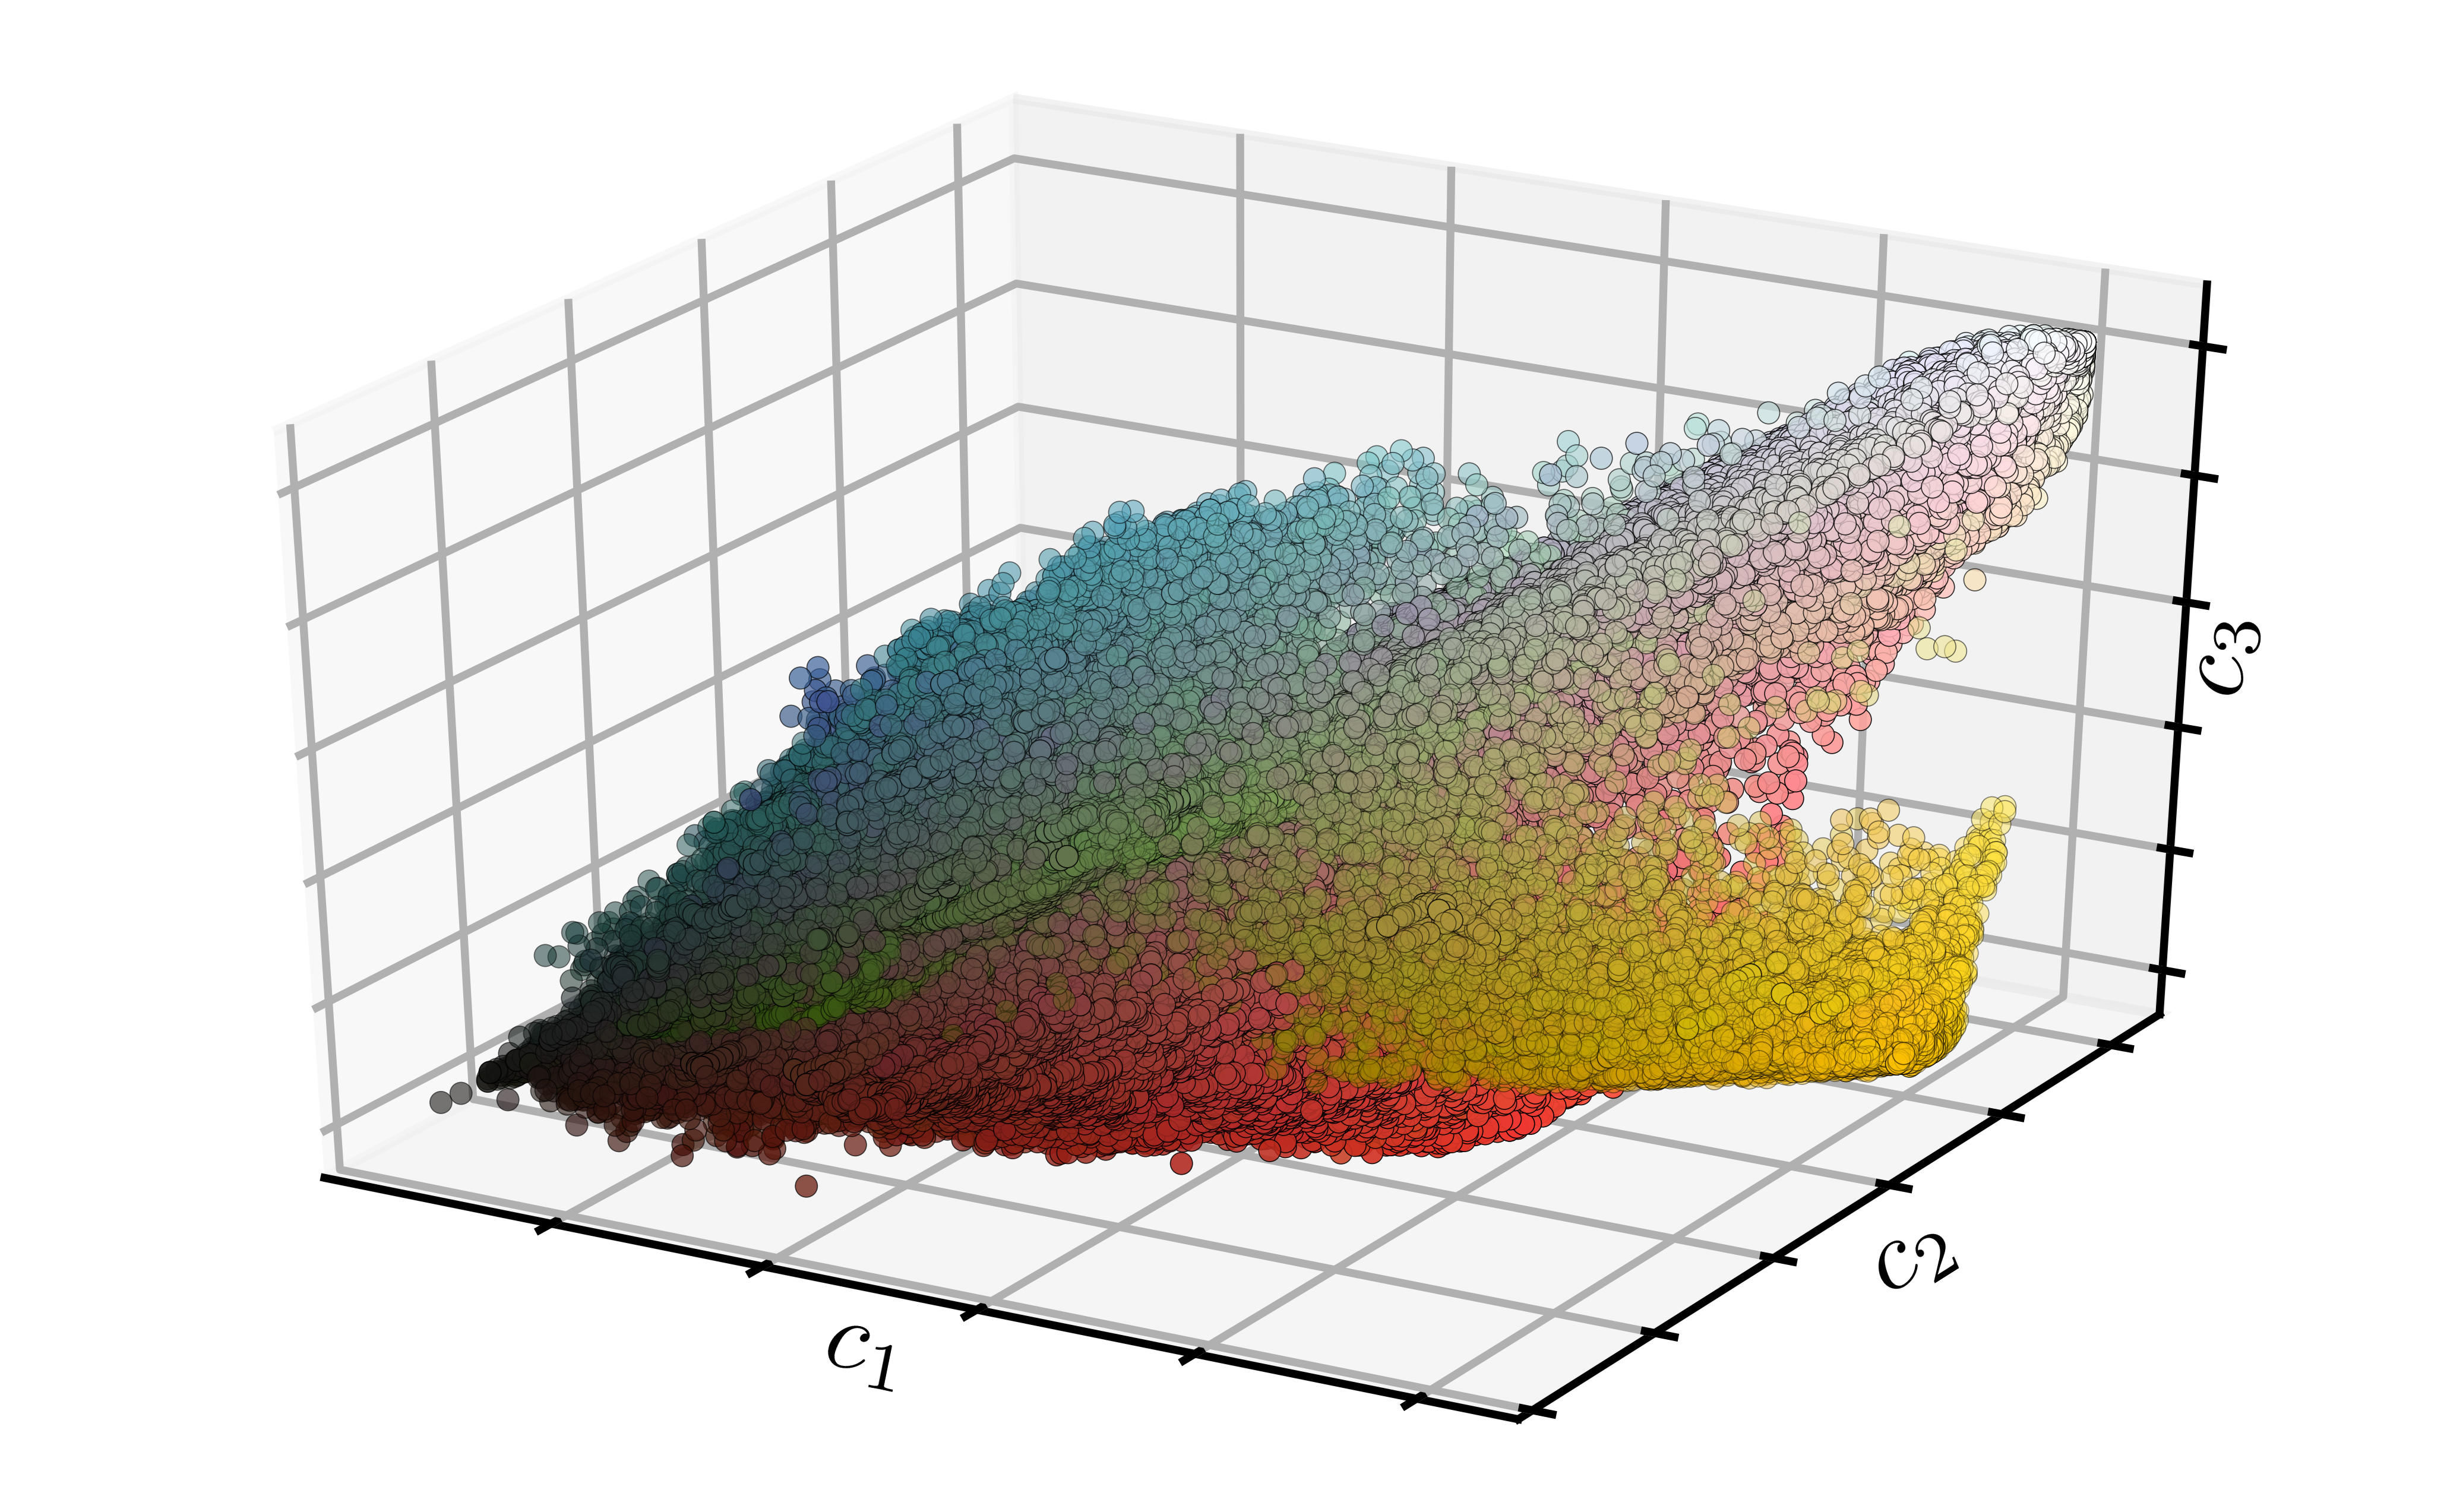
\includegraphics[width=\textwidth]{araras_3d_distribution}
        \caption{3-d image color pixel distribution}
    \end{subfigure} 
    \begin{subfigure}[b]{0.49\textwidth}
        \includegraphics[width=\textwidth]{araras_3d_histogram}
        \caption{3-d color pixel histogram}
    \end{subfigure} 
    
    \caption{3-d image color representation. 3-d pixel distribution and 10 bins 3-d pixel histogram.}\label{fig:3d_color_representation}    
\end{figure}


\subsection{Color Signature}

\begin{figure}[!ht]
    \centering
    \begin{subfigure}[b]{0.4\textwidth}
        \includegraphics[width=\textwidth]{araras}
        \caption{Input image}
    \end{subfigure} \\
    
    \begin{subfigure}[b]{0.4\textwidth}
    	\includegraphics[width=\textwidth]{araras_color_clusters}
        \includegraphics[width=\textwidth]{araras_bar_signature}
        \caption{Color signature}
    \end{subfigure}
    	~ %add desired spacing between images, e. g. ~, \quad, \qquad, \hfill etc. 
      %(or a blank line to force the subfigure onto a new line)
    \begin{subfigure}[b]{0.5\textwidth}
        \includegraphics[width=\textwidth]{araras_3d_signature}
        \caption{3-d representation of color ignature}
    \end{subfigure} 
    	    
    \caption{Image color signature and the 3-d visualization of signature clusters.}\label{fig:color_signature}    
\end{figure}



\begin{figure}[!ht]
    \centering
    \begin{subfigure}[t]{\dimexpr0.32\textwidth+20pt\relax}
    	\makebox[20pt]{\raisebox{40pt}{ \small\textbf{\textsf{(a)}} }}%
    	\includegraphics[width=\dimexpr\linewidth-20pt\relax]{tempo}
    \end{subfigure}~ 
%    \begin{subfigure}[b]{0.32\textwidth}
%        \includegraphics[width=\textwidth]{araras}
%    \end{subfigure}~
    \begin{subfigure}[b]{0.32\textwidth}
        \includegraphics[width=\textwidth]{clownfish}
    \end{subfigure}~
    \begin{subfigure}[b]{0.32\textwidth}
        \includegraphics[width=\textwidth]{mountain}
    \end{subfigure}\vspace{10pt}
    
    \begin{subfigure}[t]{\dimexpr0.32\textwidth+20pt\relax}
    	\makebox[20pt]{\raisebox{40pt}{ \small\textbf{\textsf{(b)}} }}%
    	\includegraphics[width=\dimexpr\linewidth-20pt\relax]{tempo_single_histogram}
    \end{subfigure}~     
%    \begin{subfigure}[b]{0.32\textwidth}
%        \includegraphics[width=\textwidth]{araras_single_histogram}
%    \end{subfigure}~
    \begin{subfigure}[b]{0.32\textwidth}
        \includegraphics[width=\textwidth]{clownfish_single_histogram}
    \end{subfigure}~
    \begin{subfigure}[b]{0.32\textwidth}
        \includegraphics[width=\textwidth]{mountain_single_histogram}
    \end{subfigure}\vspace{10pt}
    
    \begin{subfigure}[t]{\dimexpr0.32\textwidth+20pt\relax}
    	\makebox[20pt]{\raisebox{40pt}{ \small\textbf{\textsf{(c)}} }}%
    	\includegraphics[width=\dimexpr\linewidth-20pt\relax]{tempo_3d_distribution}
    \end{subfigure}~ 
%    \begin{subfigure}[b]{0.32\textwidth}
%        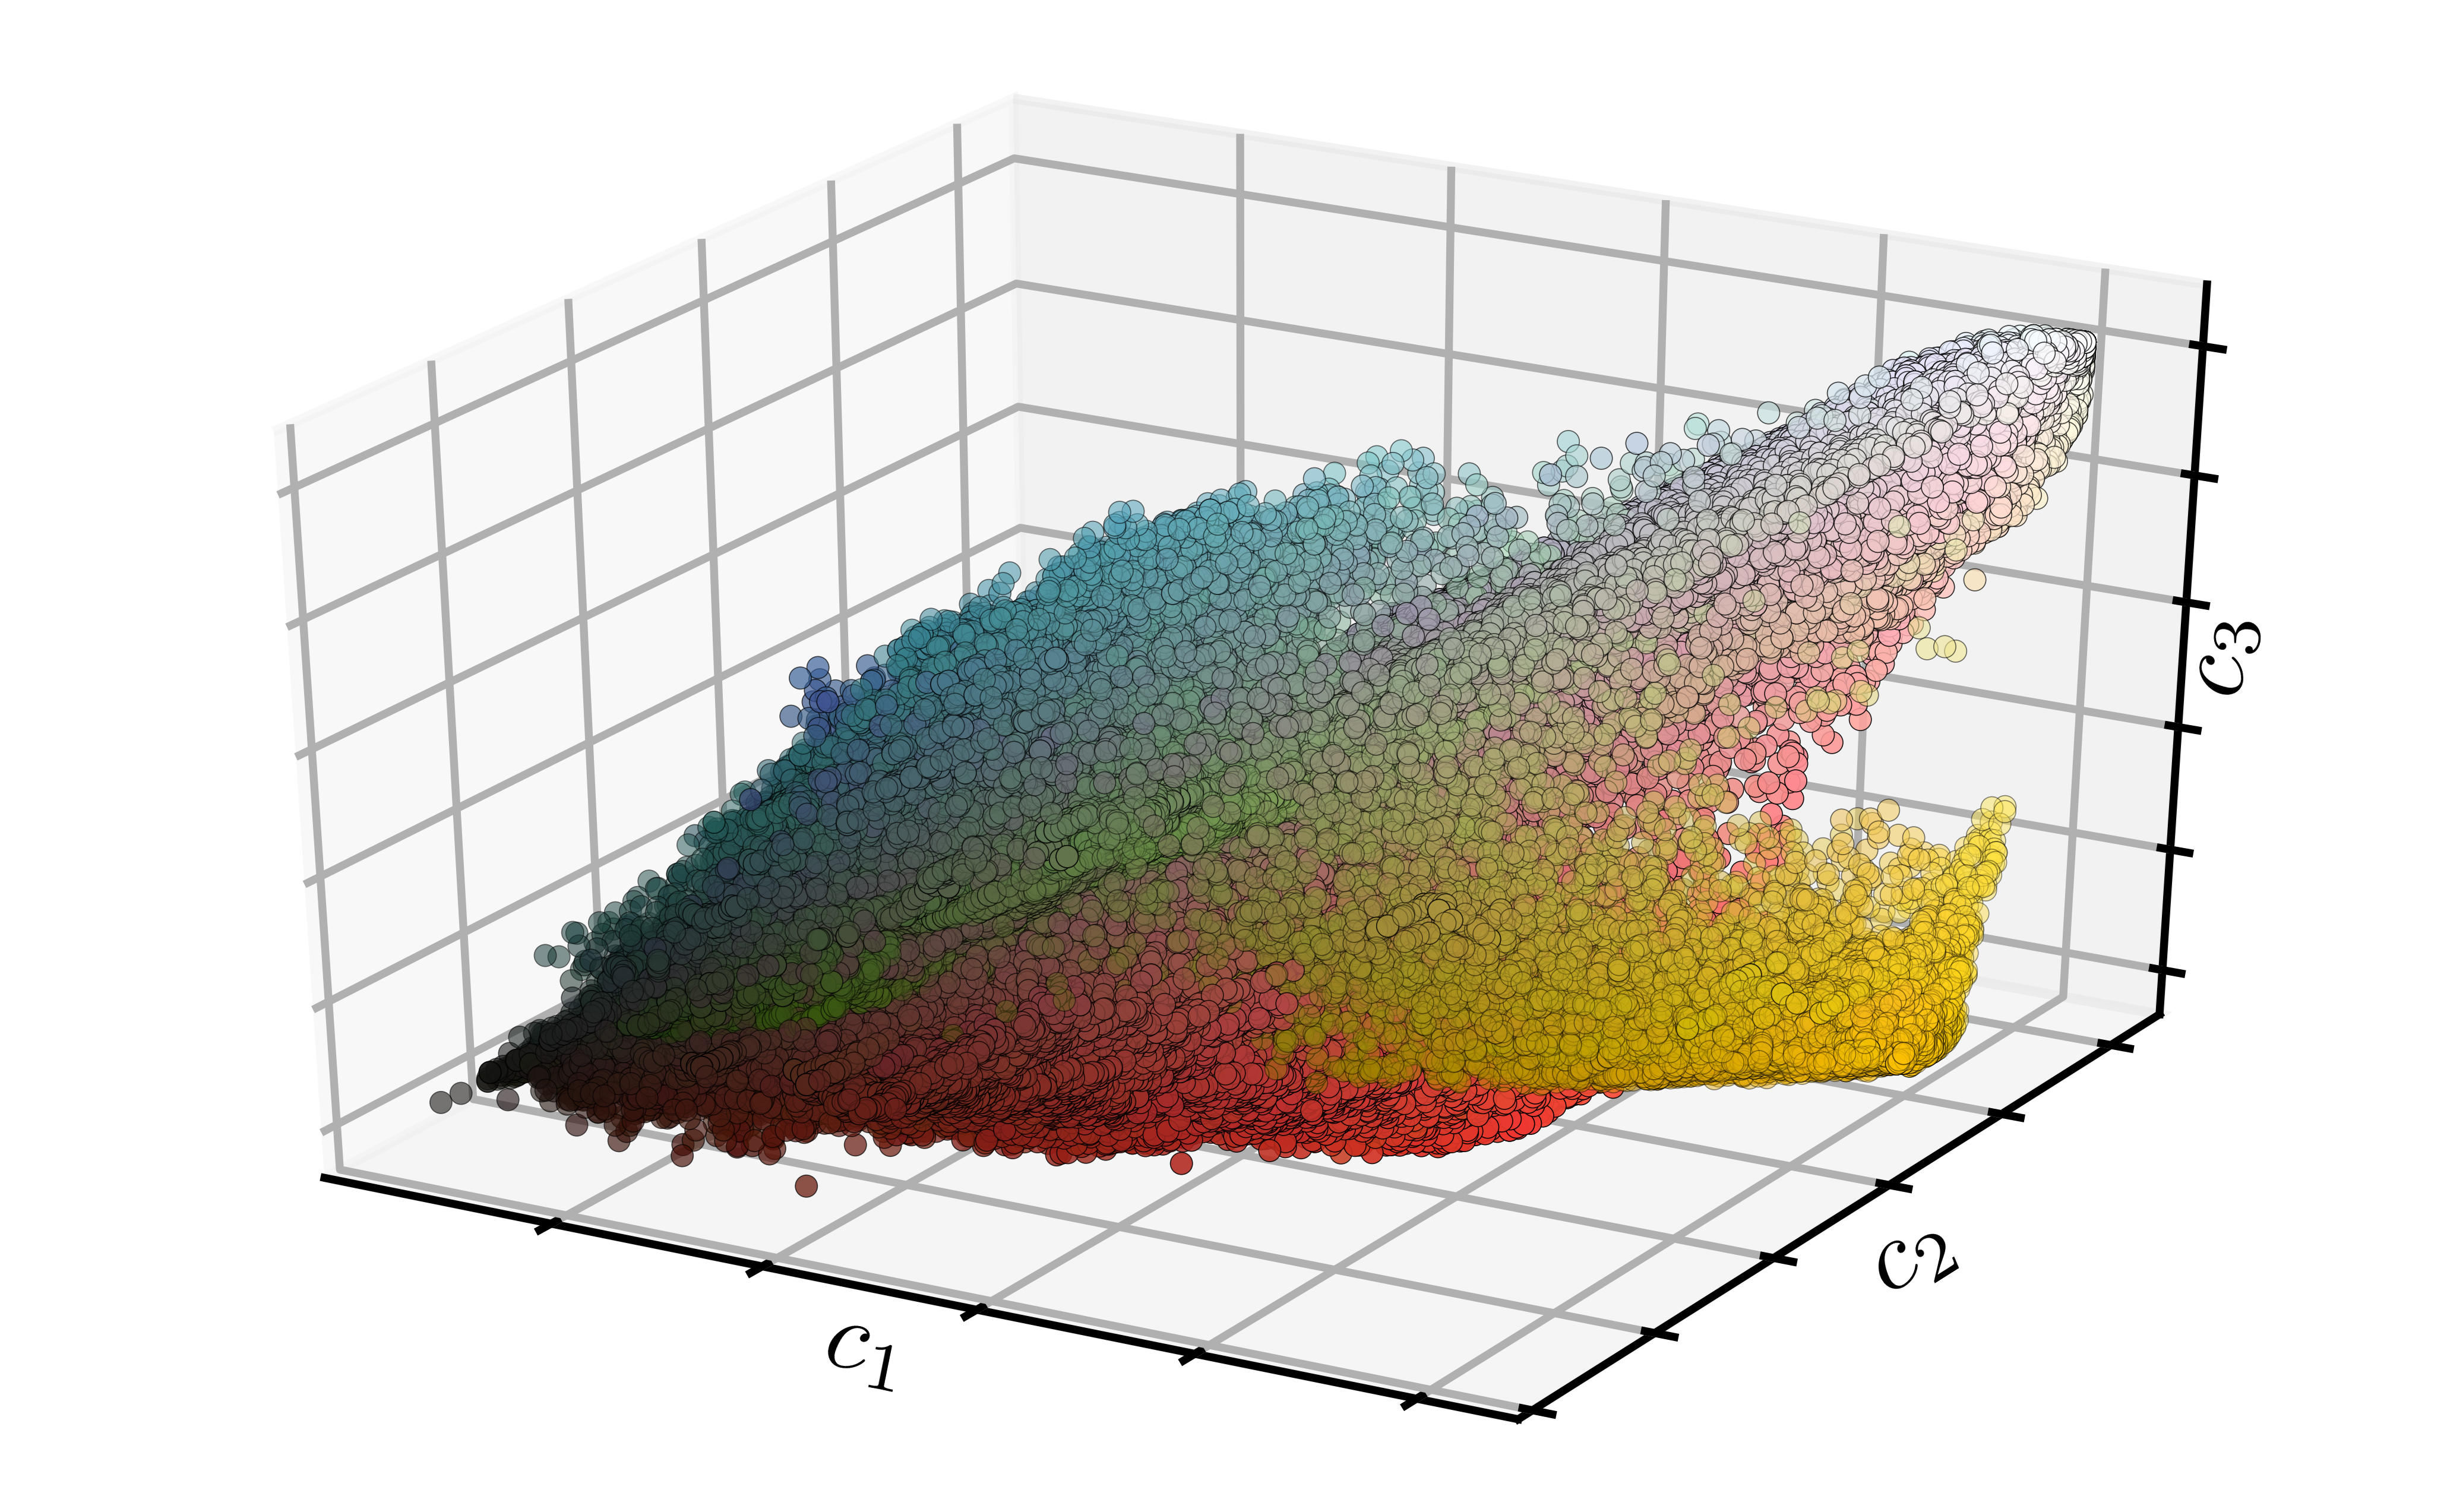
\includegraphics[width=\textwidth]{araras_3d_distribution}
%    \end{subfigure}~
    \begin{subfigure}[b]{0.32\textwidth}
        \includegraphics[width=\textwidth]{clownfish_3d_distribution}
    \end{subfigure}~
    \begin{subfigure}[b]{0.32\textwidth}
        \includegraphics[width=\textwidth]{mountain_3d_distribution}
    \end{subfigure}\vspace{10pt}
    
    \begin{subfigure}[t]{\dimexpr0.32\textwidth+20pt\relax}
    	\makebox[20pt]{\raisebox{40pt}{ \small\textbf{\textsf{(d)}} }}%
    	\includegraphics[width=\dimexpr\linewidth-20pt\relax]{tempo_3d_histogram}
    \end{subfigure}~ 
%    \begin{subfigure}[b]{0.32\textwidth}
%        \includegraphics[width=\textwidth]{araras_3d_histogram}
%    \end{subfigure}~
    \begin{subfigure}[b]{0.32\textwidth}
        \includegraphics[width=\textwidth]{clownfish_3d_histogram}
    \end{subfigure}~
    \begin{subfigure}[b]{0.32\textwidth}
        \includegraphics[width=\textwidth]{mountain_3d_histogram}
    \end{subfigure}\vspace{10pt}
    
    \begin{subfigure}[t]{\dimexpr0.32\textwidth+20pt\relax}
    	\makebox[20pt]{\raisebox{40pt}{ \small\textbf{\textsf{(e)}} }}%
    	\includegraphics[width=\dimexpr\linewidth-20pt\relax]{tempo_3d_signature}
    \end{subfigure}~ 
%    \begin{subfigure}[b]{0.32\textwidth}
%        \includegraphics[width=\textwidth]{araras_3d_signature}
%    \end{subfigure}~
    \begin{subfigure}[b]{0.32\textwidth}
        \includegraphics[width=\textwidth]{clownfish_3d_signature}
    \end{subfigure}~
    \begin{subfigure}[b]{0.32\textwidth}
        \includegraphics[width=\textwidth]{mountain_3d_signature}
    \end{subfigure}\vspace{10pt}
    
    \begin{subfigure}[t]{\dimexpr0.32\textwidth+20pt\relax}
    	\makebox[20pt]{\raisebox{40pt}{ \small\textbf{\textsf{(f)}} }}%
    	\includegraphics[width=\dimexpr\linewidth-20pt\relax]{tempo_color_clusters}
    \end{subfigure}~ 
%    \begin{subfigure}[b]{0.32\textwidth}
%        \includegraphics[width=\textwidth]{araras_color_clusters}
%    \end{subfigure}~
    \begin{subfigure}[b]{0.32\textwidth}
        \includegraphics[width=\textwidth]{clownfish_color_clusters}
    \end{subfigure}~
    \begin{subfigure}[b]{0.32\textwidth}
        \includegraphics[width=\textwidth]{mountain_color_clusters}
    \end{subfigure}\vspace{-5pt}
    
    \begin{subfigure}[t]{\dimexpr0.32\textwidth+20pt\relax}
    	\makebox[20pt]{\raisebox{25pt}{}}%
    	\includegraphics[width=\dimexpr\linewidth-20pt\relax]{tempo_bar_signature}
    \end{subfigure}~ 
%    \begin{subfigure}[b]{0.32\textwidth}
%        \includegraphics[width=\textwidth]{araras_bar_signature}
%    \end{subfigure}~
    \begin{subfigure}[b]{0.32\textwidth}
        \includegraphics[width=\textwidth]{clownfish_bar_signature}
    \end{subfigure}~
    \begin{subfigure}[b]{0.32\textwidth}
        \includegraphics[width=\textwidth]{mountain_bar_signature}
    \end{subfigure}
                    
	\caption{Different representations of color information. {\small \textsf{\textbf{(a)}}} input color image , {\small \textsf{\textbf{(b)}}} single-channel color histogram , {\small \textsf{\textbf{(c)}}} 3-d color distribution , {\small \textsf{\textbf{(d)}}} 3-d color histogram , {\small \textsf{\textbf{(e)}}} 3-d color signature , {\small \textsf{\textbf{(f)}}} color signature clusters .}\label{fig:color_image_representations}    
\end{figure}


\section{Texture}

\section{Texture characterization}

\begin{figure}[!ht]
    \centering
    \begin{subfigure}[b]{0.19\textwidth}
        \includegraphics[width=\textwidth]{brodatz_skin}
        \caption{}
    \end{subfigure}
    %~ %add desired spacing between images, e. g. ~, \quad, \qquad, \hfill etc. 
      %(or a blank line to force the subfigure onto a new line)
    \begin{subfigure}[b]{0.19\textwidth}
        \includegraphics[width=\textwidth]{brodatz_three}
        \caption{}
    \end{subfigure} 
    %~ %add desired spacing between images, e. g. ~, \quad, \qquad, \hfill etc. 
      %(or a blank line to force the subfigure onto a new line)    
    \begin{subfigure}[b]{0.19\textwidth}
        \includegraphics[width=\textwidth]{brodatz_wall}
        \caption{}
    \end{subfigure}
    %~ %add desired spacing between images, e. g. ~, \quad, \qquad, \hfill etc. 
      %(or a blank line to force the subfigure onto a new line)
    \begin{subfigure}[b]{0.19\textwidth}
        \includegraphics[width=\textwidth]{brodatz_vlines}
        \caption{}
    \end{subfigure}
    %~ %add desired spacing between images, e. g. ~, \quad, \qquad, \hfill etc. 
      %(or a blank line to force the subfigure onto a new line)
    \begin{subfigure}[b]{0.19\textwidth}
        \includegraphics[width=\textwidth]{brodatz_sponge}
        \caption{}
    \end{subfigure}\\
    
    \begin{subfigure}[b]{0.19\textwidth}
        \includegraphics[width=\textwidth]{brodatz_tissue}
        \caption{}
    \end{subfigure}
    %~ %add desired spacing between images, e. g. ~, \quad, \qquad, \hfill etc. 
      %(or a blank line to force the subfigure onto a new line)
    \begin{subfigure}[b]{0.19\textwidth}
        \includegraphics[width=\textwidth]{brodatz_cafe}
        \caption{}
    \end{subfigure} 
    %~ %add desired spacing between images, e. g. ~, \quad, \qquad, \hfill etc. 
      %(or a blank line to force the subfigure onto a new line)    
    \begin{subfigure}[b]{0.19\textwidth}
        \includegraphics[width=\textwidth]{brodatz_crystal}
        \caption{}
    \end{subfigure}
    %~ %add desired spacing between images, e. g. ~, \quad, \qquad, \hfill etc. 
      %(or a blank line to force the subfigure onto a new line)
    \begin{subfigure}[b]{0.19\textwidth}
        \includegraphics[width=\textwidth]{brodatz_flowers}
        \caption{}
    \end{subfigure}
    %~ %add desired spacing between images, e. g. ~, \quad, \qquad, \hfill etc. 
      %(or a blank line to force the subfigure onto a new line)
    \begin{subfigure}[b]{0.19\textwidth}
        \includegraphics[width=\textwidth]{brodatz_paint}
        \caption{}
    \end{subfigure}    
                  
    \caption{ Examples of texture images and its classification. [{\small \textsf{\textbf{(a) (b) (e) (h)}}}] nautural textures, [{\small \textsf{\textbf{(c) (d) (f) (g) (i) (j)}}}] man-made textures, [{\small \textsf{\textbf{(c) (d)}}}] regular textures, [{\small \textsf{\textbf{(g) (h)}}}] stochastic textures, [{\small \textsf{\textbf{(c) (d)}}}] homogeneous, [{\small \textsf{\textbf{(a) (b) (f) (g) (h)}}}] weakly-homogeneous, [{\small \textsf{\textbf{(i) (j)}}}] inhomogeneous.}\label{fig:texture_images}    
\end{figure}


\begin{itemize}
	\item Natural and artificial 
	\item Regular, stochastic
	\item Homogeneous, non-homogeneous, in-homogeneous
\end{itemize}



There is a disagreement in the definition of texture in the field of computer vision. It is possible to give a mathematical definition based on its statistical properties, however, these properties are very imprecise and/or restrictive to adapt to the diversity of existing textures.

The definition that we support is based on an experimental finding: a texture is a field of the image that appears as a coherent and homogeneous domain, that is, it forms a whole for an observer. In fact, it is this property of coherence of the texture placed in the context of being perceived as a homogeneous whole for the human eye that is most often sought for image processing, either with the aim of isolating textures, to segment the image or for the recognition of regions.

Some examples of natural textures are shown in the figure. These images come from the reference work Brodatz and show the possible variety of textures that are commonly used to test different algorithms and methods of vision.

The perception of textures is a key property of human vision. Although there is still no generalized definition, we can define texture as a measure of coarseness, contrast, directionality, line similarity, regularity and roughness. Therefore, the features that chracterize texture attempt to capture the granularity and repetition of perceptually similar patterns of surfaces within a region of the image, such that a human observer perceives the region as homogeneous.
Unlike color, texture information is not a purely pixel-level property. Texture implies the notion of spatial extent, that is, that the spatial variation of intensities of a group of pixels generate textures in the images.

There are numerous studies that review, compare and organize the work of texture analysis in different ways \citep{Materka.Strzelecki:Report:1998}, \citep{Zhang.Tan:PR:2002}, \citep{Bharati.Liu.ea:CILS:2004},\citep{Lukashevich.Sadykhov:ICPCI:2012}, \citep{Humeau-Heurtier:IEEEAccess:2019}. One possible organization is based on its operating principle, which classifies the texture characterization techniques into: statistical methods, structural method, model-based methods, transform-based methods, graph-based methods, learning-based methods and entropy-based methods. In this chapter we review five of the most widely used methods in the literature and their techniques for extracting textures fearures.

% \begin{enumerate}[noitemsep]%,topsep=0pt
%	\item Statistical methods
%	\item Structural methods
%	\item Model-based methods
%	\item Transform-based methods
%	\item Graph-based methods
%	\item Learning-based methods
%	\item Entropy-based methods
%\end{enumerate}
%	

\subsection{Statistical Methods}
Statistical methods contemplate that textures are determined by the way the gray levels are distributed over the pixels of an image. In these methods, the gray level distribution of the image is represented by a histogram.

A first approach in this category is the histogram properties analysis \citep{Aggarwal.K.Agrawal:JSIP:2012}. The first-order statistics properties are the mean and the Central Moments of the 1D histogram, that is, the variance, skewness, and kurtosis. These properties provide information on the distribution of the gray levels of the image from a global point of view, taking into account individually the gray level of the pixels. Hoewever, they do not provide any information on how the gray level of a pixel at a given location statistically affects the gray level value of another pixel at a relative location from the reference pixel.
The second-order statistical properties explore this option ang give a description of the texture, based on the comparison of intensity values of two pixels. In this case the Co-Occurrence matrix \citep{Haralick.Shanmugam.ea:TSMC:1973} is the second-level histogram that maps the intensity distribution of the pixels. Some of the texture features extracted from the second-order statistics are Angular Second Moment (ASM), Contrast, Correlation, Homogeneity, Entropy and Energy.

Local Binary Patterns (LBP) \citep{Ojala.Pietikainen.ea:PR:1996} are another technique for obtaining second-level histograms. This approach summarizes the spatial structure and local contrast of an image within a binary pattern, comparing the gray level of each pixel with its neighborhood. If the intensity value of the central pixel is greater than its neighbor, then it is denoted by 1, otherwise by 0. Subsequently, a binary array is constructed, following a consistent ordering of the neighboring values, which is transformed to decimal number and stored in a new array. The process of thresholding, construction of binary strings, binary to decimal transformation, and storing of decimal output is performed for all pixels in the image, resulting in an LPB image. Finally the second-level histogram for texture chraracterization is obtained from this resulting LBP image.

\subsection{Structural Methods}
The structural methods are based on the decomposition of the image in basic units, i.e., in elements, low-level primitives o texels. Such units can be points, lines, regions, or shapes. The basic units and their spatial arrangement in the image are used to characterize the textures. These approaches consider that textures are patterns formed by replication, more or less regular, of a basic unit. The arrangement of the primitives allows obtaining geometric relationships and subsequently statistical properties that serve serve to characterize textures. Structural tecniques aim to determine the textual primitive and define the location rules.

Dpends on the application, structural tecniques differ according to the choice of primitives. Some of the commonly considered primitives are pixels, regions of uniform intensity, line segments, or peaks in the gray level distribution. For the recovery of these primitives, highly known approaches are generally used, for example, the SIFT (Scale Invariant Feature Trasform) operator in the case of characteristic points and the contour detectors, such as Sobel and Canny, for line and edge recovery. On the other hand, the primitive's measurements and statistics most commonly used are intensity, orientation, elongation, curvature, compactness, among others.

\subsection{Model-based Methods}
This group of methods stipulates that the textures can be described by some mathematical model. This category is mainly subdivided into two approaches: stochastics and fractals.

Stochastic methods for texture modeling are very popular, in particular random field models. In this context, a texture model is a parametric family of spatially homogeneous random fields, which depend on a series of hyperparameters \citep{Winkler:Book:2003}. Inside such a family a specific texture can be characterized by a special set of hyperparameters that captures its characteristic features. According to the properties of the random fields, some of the models used for the characterization of texture are Markov Random Field (MRF) \citep{Hassner.Sklansky:CGIM:1980, Cross.Jain:PAMI:1983}, Gibbs Random Field (GRF) \citep{Derin.Cole:CVGIM:1986}, Conditional Random Field (CRF), Gaussian Markov Random Field (GMRF) \citep{Cohen.Fan.ea:PAMI:1991}.

Within the category of stochastic approaches, there is a group of techniques that use probabilistic approaches and mathematical morphology operators for the modeling of random textures \citep{Serra:CGIM:1980}, \citep{Cord.Bach.ea:JoM:2010}.

Fractal models consider textures as complex chaotic systems, so they exhibit fractal behavior. Textures, as fractal objects, have identical shape and statistical characteristics at different scales. Fractal geometry relies on self similarity across multiple scales and is measured with the fractal dimension. Fractal model-based approaches aim to determine fractal dimension, find fractal geometry, and calculate fractal measurements for the description of textures in images.


\subsection{Transform-based Methods}
Transform methods map an image to a space within which the textures are characterizable. The peculiarity is that the new space coordinates allow the interpretation of the textures because they reflect the texture properties, for example, the log-polar coordinates in the case of Gabor transform, they reflect the periodicity and orientation of the textures present in an image.

Within this category, one of the most notable methods for the extraction of texture features are Law's filter banks \citep{Laws:IUW:1979, Laws:IPMG:1980, Laws:Report:1980}. There are also the approaches based on the Fourier transform \citep{Ursani.Kpalma.ea:ICMV:2007}, where it is used to decompose the image into its frequency components. Following the same principle, there are the approaches based on Gabor decomposition \citep{Gabor:JIEE:1946} and those based on wavelets \citep{Arivazhagan.Ganesan:PR:2003}, which analyze the content of a texture not only in the frequency domain, but also in the spatial domain. On the one hand, the Gabor filter is defined as a sinusoidal wave plane modulated Gaussian kernel, which can be adapted in frequency, orientation and bandwidth. For its part, the wavelet transform allows the analysis of the texture in the frequency and spatial domain by means of the dilation and translation, respectively, of a mother wavelet.

\subsection{Learning-based Methods}
The methods for the extraction of texture features based on learning are relatively new with respect to the other methods mentioned in this work.
This category of approaches can be divided into two subclasses: the visual dictionary methods and the deep learning methods.

Visual dictionary methods are motivated by natural language processing algorithms. In this case, the aim is to generate a codebook or dictionary that contains basic geometric elements of the images, also called \textit{textons}. In the document processing analogy, textons correspond to words; so an image can be described by the repetition (organized or not) of a set of textons.

There are different strategies for calculating textons \citep{Zhu.Guo.ea:IJCV:2005}. For example, the approaches based on generative models, where an image is considered to be a linear combination of some base images. Such base images are represented by Gabor or Laplacian-of-Gaussian (LoG) functions and other wavelet transforms. Following the principle of generative models, textons are the base functions learned from a large number of image patches.
Other approaches to obtaining textons are based on discriminative modeling. In this case, the base functions are rotated and scaled filters that form a family which is convolved with the image. The responses of the filters form a feature space  in which it is possible to form clusters. Each cluster center then corresponds to a texton. To obtain a texton dictionary, it is necessary to obtain the feature space and the cluster centers from a group of training images.

Models based on deep learning use Convolutional Neural Networks (CNNs) for the extraction and representation of image features. CNNs consist of multiple locally connected layers which covolve kernels over the entire image. These approaches analyze the information of a group of images to generate a model. The characteristics of the learned model are a function of the input images, which in the case of the study of texture, is expected to generalize the properties of granularity, frequency, orientation, etc. of patterns in the training dataset.


%\section{Conclusions}


%%    \afterpage{\blankpage}
%	\cleardoublepage
%	
%	% created on 12/05/2020
% @author : ebazan

\chapter{Color Texture Analysis Based on Spectral Decomposition}\label{ch:complex_spectral_image_decomposition}
\section*{Résumé}
\noindent Dans ce chapitre, nous présentons la décomposition spectrale d'une image couleur utilisant le filtre de Gabor. Nous utilisons la théorie des fonctions de Gabor développée au chapitre \ref{ch:spectral_image_decomposition} pour extraire les caractéristiques de texture locale d'une image en couleur. La stratégie principale consiste à transformer l'image d'entrée d'un espace couleur réel à trois canaux en une représentation couleur complexe à deux canaux. Ensuite, nous utilisons une banque de filtres Gabor sur chaque canal de l'image pour extraire les informations de texture générées par les variations de couleur et d'illumination de l'image.

\section*{Abstract}
\noindent  In this chapter, we present the spectral decomposition of a color image employing the Gabor filter. We use the Gabor functions theory developed in chapter \ref{ch:spectral_image_decomposition} to extract local features of a texture color. The primary strategy involves transforming the input image from a three-channel real color space into a two-channel complex color representation. Then, we use a bank of Gabor filters on each channel of the image to extract the texture information generated by the variations of color and illumination in the image. 

\section{Introduction}

Gabor filters have long been used for analyzing textures and extracting corresponding image features. Its adaptability and customization, depending on the application and the relationship with the human visual system  \citep{Daugman:JOSA:1985a}, have made this technique one of the most relevant for analyzing textures in an image. 

The use of Gabor filters for image texture analysis is highly dependent on the final application. Some of the most recognized works in the literature date back to the late 90s, where this technique was a hot research topic for image texture analysis. However, regarding the works present in the literature, we can separate the methods taking into account the nature of the extracted features. The first group uses Gabor filters to extract a global texture descriptor (Gabor signature). Generally, this strategy is suitable for applications where the images contain homogeneous textures, and it is sought to make the classification of images or an image retrieval system based on the content, as we can see in chapter \ref{ch:similarity_measures}. The second group is characterized by using Gabor filters to obtain local texture features present in an image. Such a strategy is suitable for image segmentation tasks. In this chapter, we address the second case straightforwardly and comprehensively, delving into the spectral decomposition of color images to obtain texture features generated by the changes in illumination and (or) color.

We take advantage of the Gabor function's dual-domain (spatial and frequency) representation capability to create a bank of filters $G=\{g_{f, \theta}(x, y) \}$ and obtain the spectral decomposition of an input image $I(x, y)$ through the convolution operation of each of the filters such that 
\begin{equation}\label{eq:gabor_responses}
    r_{f, \theta}(x,y) = I(x, y) \ast g_{f, \theta}(x,y)
\end{equation}
represents the filter response at different central frequencies $f$ (scales) and orientations $\theta$. Given the complex form of Gabor filters Eq. \eqref{eq:gabor_function_2d_spacefreq_bank} defined in chapter \ref{ch:spectral_image_decomposition}, the filter response $r_{f,\theta}(x, y)$ has a real and an imaginary part, here denoted as $\RE{(\cdot)}$ and $\IM{(\cdot)}$, respectively.

The linear transformation of an image using Eq. \eqref{eq:gabor_responses}, produces considerable information about the image's textures. The efficient manipulation of this information is the basis for extracting appropriate (local or global) texture features. Although the image's convolution by a filter bank is a common denominator in techniques based on signal processing, in the literature, we find various options to create more separable texture features (see Fig. \ref{fig:general_pipeline_gabor_feature_extraction}). In general, these methods differ in the type of output they use to measure the image's textural information and the post-processing techniques to refine the Gabor responses. Among the possible Gabor filter responses to measure the texture information, some of the most used in the literature are

\begin{enumerate}
    \item The amplitude of the response (magnitude or Gabor energy) \citep{Bovik.Clark.ea:TPAMI:1990}.
        \begin{equation}\label{eq:gabor_magnitude}
            |r_{f, \theta}(x,y)| = \sqrt{\RE{(r_{f, \theta}(x, y))}^2 + \IM{(r_{f, \theta}(x, y))}^2}
        \end{equation}
    \item The phase of the response \citep{Palm.Lehmann:MGV:2002}.
    \begin{equation}\label{eq:gabor_phase}
            \arg(r_{f, \theta}(x,y)) = \arctan2{\left(\frac{\IM{(r_{f, \theta}(x, y))}}{\RE{(r_{f, \theta}(x, y))}}\right)}
        \end{equation}
    \item The real component of the response \citep{Jain.Farrokhnia:IJPR:1991}.
    \begin{equation}\label{eq:gabor_real_part}
            \RE{(r_{f, \theta}(x, y))}
        \end{equation}
    \item The square amplitude of the response (Gabor local power spectrum) \citep{Grigorescu.Petkov.ea:TIP:2002}.
    \begin{equation}\label{eq:gabor_power}
            |r_{f, \theta}(x,y)|^2 = \RE{(r_{f, \theta}(x, y))}^2 + \IM{(r_{f, \theta}(x, y))}^2
        \end{equation}
\end{enumerate}
while the most common post-processing techniques for the filter outputs consist of a non-linear transformation followed by smoothing using a rectangular or Gaussian window \citep{Randen.Husoy:TPAMI:1999}, \citep{Clausi.EdJernigan:JPR:2000}. The application of non-linearity favors the activation of the textured areas in the images, while the smoothing favors the location of the energy obtained with the filter, avoiding the loss of information from the natural contours of the image. Figure \ref{fig:general_pipeline_gabor_feature_extraction} illustrates the stages (boxes with continuous black lining) and the input/outputs (boxes with black dotted lining) of the scheme mentioned above, referring to the extraction of Gabor-based texture features. 

\begin{figure}[!ht]
	\centering
	\includegraphics[width=\textwidth]{general_pipeline_gabor_feature_extraction}
	\caption{Pipeline of classic techniques for extraction of texture features using the Gabor filters. }\label{fig:general_pipeline_gabor_feature_extraction}
\end{figure}


\subsection{Texture features for color images}
Most of the research work on texture has been done using gray-scale images and with homogeneous textures; see for example \citep{Jain.Farrokhnia:IJPR:1991}, \citep{ChengjunLiu.Wechsler:NN:2003}, \citep{Liu.Koga.ea:ICDAR:2005}, \citep{Al-Kadi:arXiv:2017}. Consequently, the simplest way to obtain texture features from color images is to transform them into a gray-scale image. This strategy favors the acceleration of feature calculation because we work with scalar values instead of vectors. However, despite the good results in images with homogeneous gray-scale textures, reducing channels for a natural-color image with non-homogeneous textures does not ensure the generation of representative texture features. This outcome is primarily because the non-homogeneous textures in a color image are generated by luminance variations and variations in chromaticity. Moreover, the real-world scenes are in color and contain non-homogeneous textures.  For example, in the case of a texture image in the RGB color space, which its gray-scale transformation represents the levels of red, green, and blue \citep{Artusi.Banterle.ea:Book:2016} as
%L = 0.2126 R + 0.7152 G + 0.00722 B
\begin{equation}\label{eq:color2gray_formula}
    L = 0.299 R + 0.587 G + 0.114 B    
\end{equation} 
if the image contains isoluminant colors (colors with the same luminance value), the transformation $L$ leads to a minimization or lost, in the worst case, of textures generated by the color changes.
%\textit{Idea to develope:} Illustrate the effect of compute unichrome features in the gray-scale and the RGB space for a color image.

% for a colored real-world image containing non-homogeneous textures. 
% Although there is some texture information in the color input image,

Notwithstanding, we find a large number of methods that propose the characterization of textures in color images. Such methods generally use two strategies for the analysis of color textures \citep{Maenpaa.Pietikainen:PR:2004}, \citep{Qazi.Alata.ea:PR:2011}:

\begin{itemize}
	\item process color and texture information separately
	\item process color and texture as a joint phenomenon
\end{itemize} 

The first category methods assume that the spatial variations that form textures and color distributions of the image are independent cues (see for example \citep{Permuter.Francos.ea:PR:2006}). We differ from this point of view, and we consider that color and texture information in an image is a joint phenomenon based on the idea that textural segmentation occurs based on the distribution of simple properties of texture elements, for example, the brightness, color, size, and the slopes of contours and other elemental descriptors of a texture \citep{Werner.Chalupa:Book:2004}.
 
In this regard, there are various techniques to joint color and texture information to characterize natural color textures. A popular option is to get unichromatic texture features from each color channel of the image using, for example, Gabor filters. Taking the RGB color space as a reference, the filter responses represent the texture features of each primary color red, green, and blue independently, i.e., in principle, this strategy does not involve the correlation between RGB band colors. This strategy might be corrected using the opponent color model based on the human color vision theory \citep{Jain.Healey:TIP:1998}. In such a case, each unichromatic feature vector (RGB-feature) is multiplied and normalized by the feature vector of its opponent color to include the correlation between color channels \citep{Palm.Keysers.ea:JCIS:2000}. This method manages to gather the information of color and texture under a frame of human color perception. However, the normalization and multiplication of the unichromatic texture feature vectors imply extra post-processing steps in the features extraction pipeline.  

One way to avoid the post-processing stage after the image Gabor decomposition is to first transform the color image in a color space that handles the coupling between the color channels rather than separating them as individual components of the color space. The quaternion framework \citep{Sangwine.Ell:VISP:2000} provides this possibility of coupled color representation. It encodes the color value of each pixel in a pure quaternion, where the real component is set to zero, and the three imaginary components represent the color band, such as $I(x, y) = R (x, y) \mathsf{i} + G (x, y) \mathsf{j} + B (x, y) \mathsf{k}$. This 3-component vector representation yields a system with well-defined mathematical operations, such as Quaternion Fourier Transform, that makes the Gabor image decomposition possible through the Quaternion Gabor Filters (QBF) \citep{Subakan.Vemuri:EMMCVPR:2009}. However, when using quaternion values, the non-existing commutativity must be considered; the QGF does not support any physic interpretation of what is measured. 

Another alternative to this problem is to represent the image in one of the two-channel color spaces, previously defined in chapter \ref{ch:color_texure_representations}, where one channel contains the luminance information and the other the chrominance information of the image. We can obtain such a representation from the non-linear color spaces like LAB or LUV and HSV or HSL perceptual color spaces. The representation in the form of luminance-chrominance has the characteristic of concentrating the color information in a complex channel, which is compatible with the multispectral Gabor decomposition. In both cases, the choice of a pertinent color space for the texture's characterization is necessary \citep{Qazi.Alata.ea:PR:2011}.

The methodology we present in this chapter mainly follows the stages shown in the diagram of figure \ref{fig:general_pipeline_gabor_feature_extraction}. We introduce some modifications to exploit the color and texture information in the same framework. The modifications proposed to this scheme are transforming the input image from the RGB color space to one of the luminance-chrominance spaces (or complex two-channel color spaces) described in chapter \ref{ch:color_texure_representations}. Then, the non-linear transformation was replaced by a morphological opening followed by an adaptive Gaussian smoothing to highlight the amplitude of the filter responses. Under this configuration, we obtain a spectral decomposition of the image that considers the textures generated by changes in lighting and those generated by color changes. Figure \ref{fig:proposed_pipeline_gabor_feature_extraction} shows the stages we perform for the extraction of local features.

Later in the chapter, we apply the Gabor feature space for the segmentation of natural color images. 

\begin{figure}[!ht]
	\centering
	\includegraphics[width=\textwidth]{gabor_color_feature_extraction_diagram}
	\caption{The proposed methodology for the computation of Gabor features in color images.}\label{fig:proposed_pipeline_gabor_feature_extraction}
\end{figure}

%\section{Spectral decomposition of color images}
\section{Gabor Filter-based Texture Feature Space}

\subsection{Color Image Transformation}
The first stage in creating the feature space is transforming the input image from the RGB color space to the two-channel luminance-chrominance space. The representation in two channels, one real and the other complex, of a color image, allows us to separate the intervention of luminance and colors in the generation of textures in an image. To help visualize such a joint phenomenon, we create a synthetic image that reflects the complexity of natural color images.

\subsubsection{Synthetic image description}
The synthetic image we create contains seven different regions with spatial variations (textures) generated by alternating various colors at different frequencies. Each tile of the image is perceived as a whole; this is perceptually a constant region. The colors alternate along different directions in the chrominance phase (Fig. \ref{fig:color_complex_plane}). The last image region has two frequency components.

We generate the input image with the sign function of a 2-d sinusoidal signal multiplied by the color values of each region in the RGB color space such that
\begin{gather}
	I(x, y) = sgn( \sin 2 \pi (f_x x_r + f_y y_r)) \cdot [R, G, B]\label{eq:2D_squared_signal}\\
	x_r = x \cos\theta + y \sin\theta \nonumber \\
    y_r = -x \sin\theta + y \cos\theta \nonumber  
\end{gather}

We control the image texture by varying the frequencies $f_{x}, f_{y}$ and the orientation angle $\theta$ of the coordinate plane $(x, y)$, where $\theta=0^\circ$ means vertical variations and $\theta=90^\circ$ horizontal variations. The proposed image has a size of $320\times1400$ pixels. The seven characteristic regions of the image are spread over $1400$ pixels wide, so each region is about $320\times200$ pixels, that is, the color/texture distribution in the image changes every 200 pixels (on the $x$-axis). The following expressions define the image spatial variations.  
\begin{gather}
	f_{x} = 
	\begin{cases} 
      0    & 0\leq x\leq 200  \\
      1/64 & 201\leq x\leq 400  \\
      1/32 & 401\leq x\leq 600  \\
      1/16 & 601\leq x\leq 800  \\
      1/8  & 801\leq x\leq 1000  \\
      1/4  & 1001\leq x\leq 1200 \\   
      1/8  & 1201\leq x\leq 1400 \\ 
   	 \end{cases} \nonumber ; \quad
   	 f_{y} = \begin{cases} 
      0    & 0\leq x\leq 200  \\
      0    & 201\leq x\leq 400  \\
      0    & 401\leq x\leq 600  \\
      0    & 601\leq x\leq 800  \\
      0    & 801\leq x\leq 1000  \\
      0    & 1001\leq x\leq 1200 \\  
      1/32 & 1201\leq x\leq 1400 \\ 
   	 \end{cases} \nonumber  
\end{gather}

For comprehension purposes, we use colors easily identified in the RGB space (primary colors) or in the HSV space (perceptual colors) to generate the image textures. Figure \ref{fig:synthetic_color_texture_image} depicts the resulting synthetic image. 

\begin{figure}[!ht]
    \includegraphics[width=\textwidth]{synthetic_image_color_texture}
\caption{Synthetic color textured image.}\label{fig:synthetic_color_texture_image}
\end{figure}

The 2-d sinusoidal modulations generates textures in the image at a different and well known frequencies. These modulations change the colors of the regions generating a texture of oriented lines. The regions of the synthetic image have the following color and texture characteristics.

\paragraph{Region 1. Textureless zone:}
This region does not contain spatial variations, i.e., it has only a solid color. The color of the region is yellow (arbitrarily chosen).

\paragraph{Region 2. Lowest frequency textured zone with colors on the imaginary plane:}
This region is described by the vertical texture generated by variations between purple and green lime. Such colors are found in the imaginary axis of the chrominance plane. The colors in this region change every 64 pixels (along the $x$-axis).

\paragraph{Region 3. Textured zone with colors on the real plane:}
This region contains a vertical texture generated by the variations between red and cyan. Such colors are found in the real axis of the chrominance plane. The colors in this region change every 32 pixels (along the $x$-axis).

\paragraph{Region 4. Textured zone with two primary colors:}
The horizontal texture of this region is generated by the variations between red and blue. The colors in this region change every 16 pixels (along the $x$-axis). 

\paragraph{Region 5. Textured zone with two primary colors:}
The horizontal texture of this region is generated by the variations between blue and green. The colors in this region change every 8 pixels (along the $x$-axis). 

\paragraph{Region 6. Textured zone with two primary colors:}
The horizontal texture of this region is generated by the variations between green and red. The colors change every 4 pixels (along the $x$-axis).

\paragraph{Region 7. Colorless mixed textures zone:}
This region contains two textures, both of them formed by the variations between black and white, i.e., there is no color information. Moreover, the textures change in frequency and orientation; the pixes of the horizontal texture change of color every 4 pixels along the $x$-axis (highest frequency), while the pixel values of the vertical texture changes every 16 pixels along the $y$-axis (same frequency as region 4).

We summarize the colors and frequency of each zone in Table \ref{tab:synthetic_image_components}. In the table, we expose the $RGB$ and $HSV$ values of the texture-forming colors as well as the frequency and orientation of each section.


\begin{table}[!h]
\resizebox{\textwidth}{!}{%
\begin{tabular}{c|ccccccc}
                    & \multicolumn{7}{c}{\textbf{Region}}                                                                                                                                                                          \\ \hline
\textbf{}           & 1                  & 2                   & 3                   & 4                   & 5                   & 6                   & 7                                                              \\ \hline
\textbf{Color 1}    &                    &                     &                     &                     &                     &                     &                                                                \\
\textit{Name}       & Yellow             & Purple              & Red                 & Red                 & Blue                & Green               & Black                                                          \\
\textit{RGB values} & {[}255, 255, 0{]}  & {[}128, 0, 255{]}   & {[}255, 0, 0{]}     & {[}255, 0, 0{]}     & {[}0, 0, 255{]}     & {[}0, 255, 0{]}     & {[}0, 0, 0{]}                                                  \\
\textit{HSV values} & {[}60, 100, 100{]} & {[}270, 100, 100{]} & {[}0, 100, 100{]}   & {[}0, 100, 100{]}   & {[}240, 100, 100{]} & {[}120, 100, 100{]} & {[}0, 0, 0{]}                                                  \\ \hline
\textbf{Color 2}    &                    &                     &                     &                     &                     &                     &                                                                \\
\textit{Name}       & -                  & Green lime          & Cyan                & Blue                & Green               & Red                 & White                                                          \\
\textit{RGB values} & -                  & {[}128, 255, 0{]}   & {[}0, 255, 255{]}   & {[}0, 0, 255{]}     & {[}0, 255, 0{]}     & {[}255, 0, 0{]}     & {[}255, 255, 255{]}                                            \\
\textit{HSV values} & -                  & {[}90, 100, 100{]}  & {[}180, 100, 100{]} & {[}240, 100, 100{]} & {[}120, 100, 100{]} & {[}0, 100, 100{]}   & {[}0, 0, 100{]}                                                \\ \hline
\textbf{Texture}    &                    &                     &                     &                     &                     &                     &                                                                \\
\textit{Freq.}      & -                  & $1/64$              & $1/32$              & $1/16$              & $1/8$               & $1/4$               & \begin{tabular}[c]{@{}c@{}}$1/8$\\ $1/32$\end{tabular}         \\
\textit{Angle}      & -                  & $90^\circ$          & $90^\circ$          & $90^\circ$          & $90^\circ$          & $90^\circ$          & \begin{tabular}[c]{@{}c@{}}$0^\circ$\\ $90^\circ$\end{tabular}
\end{tabular}}
\caption{Specifications of the color and texture settings for each of the regions within the synthetic image.}\label{tab:synthetic_image_components}
\end{table}




%\begin{table}[h!]
%\resizebox{\textwidth}{!}{%
%\begin{tabular}{c|c|c|c|c|c|c|c|c|}
%\cline{2-9}
%\textbf{}                                & \multicolumn{6}{c|}{\textbf{Colors}}                                                                                                                                        & \multicolumn{2}{c|}{\multirow{2}{*}{\textbf{Texture}}} \\ \cline{2-7}
%                                         & \multicolumn{3}{c|}{\textbf{Color 1}}                                            & \multicolumn{3}{c|}{\textbf{Color 2}}                                                    & \multicolumn{2}{c|}{}                                  \\ \hline
%\multicolumn{1}{|c|}{\textbf{Zone}}      & \textbf{Name}          & \textbf{$RGB$ values}      & \textbf{$HSV$ values}      & \textbf{Name}          & \textbf{$RGB$ values}            & \textbf{$HSV$ values}        & \textbf{Freq.}             & \textbf{Angle}            \\ \hline
%\multicolumn{1}{|c|}{1}                  & Yellow                 & $[255,255,0]$              & $[60,100,100]$             & n/a                    & n/a                              & n/a                          & n/a                        & $90^\circ$                \\ \hline
%\multicolumn{1}{|c|}{2}                  & Purple                 & $[128, 0, 255]$            & $[270,100,100]$            & Green lime             & $[128, 255, 0]$                  & $[90,100,100]$               & $\frac{1}{64}$             & $90^\circ$                \\ \hline
%\multicolumn{1}{|c|}{3}                  & Red                    & $[255,0,0]$                & $[0,100,100]$              & Cyan                   & $[0,255,255]$                    & $[180,100,100]$              & $\frac{1}{32}$             & $90^\circ$                \\ \hline
%\multicolumn{1}{|c|}{4}                  & Red                    & $[255,0,0]$                & $[0,100,100]$              & Blue                   & $[0,0,255]$                      & $[240,100,100]$              & $\frac{1}{16}$             & $90^\circ$                \\ \hline
%\multicolumn{1}{|c|}{5}                  & Blue                   & $[0,0,255]$                & $[240,100,100]$            & Green                  & $[0,255,0]$                      & $[120,100,100]$              & $\frac{1}{8}$              & $90^\circ$                \\ \hline
%\multicolumn{1}{|c|}{6}                  & Green                  & $[0,255,0]$                & $[120,100,100]$            & Red                    & $[255,0,0]$                      & $[0,100,100]$                & $\frac{1}{4}$              & $90^\circ$                \\ \hline
%\multicolumn{1}{|c|}{\multirow{2}{*}{7}} & \multirow{2}{*}{Black} & \multirow{2}{*}{$[0,0,0]$} & \multirow{2}{*}{$[0,0,0]$} & \multirow{2}{*}{White} & \multirow{2}{*}{$[255,255,255]$} & \multirow{2}{*}{$[0,0,100]$} & $\frac{1}{4}$              & $90^\circ$                \\ \cline{8-9} 
%\multicolumn{1}{|c|}{}                   &                        &                            &                            &                        &                                  &                              & $\frac{1}{32}$             & $0^\circ$                 \\ \hline
%\end{tabular}}
%\caption{Specifications of color and texture of the areas of the synthetic study image.}\label{tab:synthetic_image_components}
%\end{table}

\subsubsection{Graphical display of the synthetic image color distribution}
The choice of texture-forming colors comes from the interest in visualizing the color spectrum of the image more graphically. The two-channel color spaces, described in chapter \ref{ch:color_texure_representations}, encode color information in a complex chrominance channel. Therefore, we can interpret the chrominance values as points within a complex plane (see Fig. \ref{fig:color_complex_plane}). In the case of LAB/LUV spaces, the values of chrominance are defined in Cartesian coordinates as 
\begin{equation}\label{eq:chrominance_lab2}
    C = A + \mathsf{i}B
\end{equation}
where channel A values represent the real axis coordinates, and channel B values represent the imaginary axis coordinates. 

HSV/HSL color spaces encode chrominance values as points in polar coordinates 
\begin{equation}\label{eq:chrominance_hsv2}
    C = S \mathsf{e}^{\mathsf{i}H}
\end{equation}
where channel H values are the angle expressed radians and channel S values are the distance from the origin to the color points.

Considering these two chrominance configurations, the one defined by hue and saturation provides a more straightforward geometric interpretation of chrominance. Originally hue is a cylindrical dimension representing the color tints in the chromatic circle as angles, while saturation, which represents the purity of color, places achromatic tints in the center of the circle and pure colors on the circular edge of the disk. In figure \ref{fig:color_complex_plane}, we show the synthetic image color distribution plot using the HS dimensions in the 2-d chrominance complex plane. The hue $H$ is expressed in degrees, and saturation $S$ is normalized between $0$ and $255$. This representation complements the description of our synthetic test image Fig. \ref{fig:synthetic_color_texture_image}, showing the variation between colors that generate textures. We can notice in the chroma circle of figure \ref{fig:color_complex_plane} the transition between the red-green-blue primary colors at $0^\circ$, $120^\circ$ and $240^\circ$ respectively; the transition between purple and lime green on the imaginary axis with a hue of $90^\circ$ and $270^\circ$ respectively; the transition between red at $0^\circ$ and cyan at $180^\circ$ passing through the real axis of the plane and finally; the yellow color with a hue value of $60^\circ$.

\begin{figure}[!ht]
	\centering
    \includegraphics[width=0.8\textwidth]{color_complex_plane}
	\caption{Synthetic image chrominance distribution represented in the color complex plane.}\label{fig:color_complex_plane}
\end{figure}

Under this color space configuration, the colors of an image are represented in the complex chrominance plane. However, in this plane, the variations due to luminance information do not appear. The brightness of the colors is captured in the luminance channel. Depending on the color space that we use to build the two-channel color representation, we can obtain the luminance channel in different ways. In the LAB/LUV and HSL color spaces, the luminance channel is directly represented by the values of the $L$ dimension. In the HSV color space, we use the image transformation from RGB to gray-scale following the Eq. \eqref{eq:color2gray_formula} to obtain the luminance channel.

Figure \ref{fig:three_channel_decomposition} shows the three dimensions of the two-channel representation of the synthetic image ($L(x,y)$, $\RE(C(x,y))$, $\IM(C(x,y))$) in grayscale. In this representation, we use the HSV color space as a basis to obtain the luminance and chrominance values, so the $L$ channel is obtained with Eq. \eqref{eq:color2gray_formula} and the $C$ channel with Eq. \eqref{eq:chrominance_hsv2}. In figure \ref{fig:three_channel_decomposition}, we can see how the different regions show more or less important values depending on the channel in which they are. For example, the horizontal and vertical spatial variations of region 7 (between 1200 and 1400 column pixels) are only visible in the luminance channel $L(x,y)$ (see left image in \ref{fig:three_channel_decomposition}). We observe this same effect in the chrominance channels, for example, with the vertical textures of region 3. The spatial variations of this region are made up by the alternation of colors that live only in the real plane of chrominance (red and cyan), so the texture is only visible in channel $\RE(C(x,y))$ (see column pixels between 400 and 600 of the central image and the image to the right of subfigure \ref{fig:three_channel_decomposition}). 

We can also visualize the color variations and their influence on the generation of textures by plotting a horizontal line using a row of pixels' intensity values for each dimension of the two-channel space. In figure \ref{fig:horizontal_line_three_channel_decomposition}, we show the variations generated by changes in color and (or) lightness in a 1-d plot. Taking the area without texture (region 1), the horizontal line between pixels 0 and 200 remains constant in all three channels due to the absence of texture. However, in region 2, which corresponds to the low-frequency texture formed by the colors at $90^\circ$ and $270^\circ$ in the chroma circle, we see that variations are only present in the imaginary channel of chrominance $\IM(C(x,y))$. In regions 4, 5, and 6, since the texture-forming colors are two of the three primary colors (red, green, blue), the variations are visible in all three luminance-chrominance representation channels. Finally, in the last region (colorless mixed textures zone), we can see that the variations are only present in the channel that describes the luminance $L(x,y)$.

\begin{figure}[!ht]
\centering
    \subcaptionbox{\label{fig:synthetic_image_three_channel_decomposition}}{\includegraphics[width=\textwidth]{synthetic_image_three_channel_decomposition}}
    \subcaptionbox{\label{fig:horizontal_line_three_channel_decomposition}}{\includegraphics[width=\textwidth]{horizontal_line_three_channel_decomposition}}    
\caption{Illustration of the proposed synthetic image: \captext{(a)} Luminance and chrominance decomposition; \captext{(b)} Numerical values on a horizontal line cut through the three channels.}\label{fig:three_channel_decomposition}
\end{figure}


\subsection{Spectral Image Decomposition}
 The first stage of our methodology for color-textured images' characterization consists of representing the input image in a two-channel luminance and chrominance space. Once we represent the image in this space, we obtain the spectral decomposition of each image dimension using a family of optimized Gabor filters (shown in figure \ref{fig:gabrfilter_5f_4a}). Following this strategy, we measure the spatial variations generated by luminance and chrominance individually. 

\begin{figure}[!ht]
    \centering
    \includegraphics[width=0.6\textwidth]{GaborFilterbank_5f_4a}
    \caption{Gabor filter bank with filters at five frequencies $f$ and four orientations $\theta$ used to model the synthetic image textures.}\label{fig:gabrfilter_5f_4a}    
\end{figure}

Among the different strategies to model the texture information with the Gabor filters listed above, we used the amplitude filter response Eq. \eqref{eq:gabor_magnitude} such that
\begin{equation}\label{eq:gabor_energy}
	e_{c, f, \theta}(x,y) = |r_{c, f, \theta}(x,y)|
\end{equation}
represents the Gabor energy captured by a Gabor filter set at frequency $f$ and orientation $\theta$ for every color channel  $c=\{L, \RE(C, \IM(C)\}$. 

The responses generated by Eq. \eqref{eq:gabor_energy} represent the raw Gabor responses, that is, without any post-processing. Although the Gabor filters we use are optimized (see chapter \ref{ch:spectral_image_decomposition} for more details on filter optimization) to capture the most information by reducing the trade-off between the spatial-frequency domains, the raw responses lack homogeneity, especially at low frequencies, where the filter support is longer. Figure \ref{fig:synthetic_img_gresponses} shows the raw Gabor responses at different frequencies and orientations of the channels of the luminance-chrominance space. 

\begin{figure}[!ht]
    \centering
    \begin{subfigure}[b]{\textwidth}   
        \includegraphics[width=\textwidth]{gabor_resp_lum_synthetic}
        \caption{$e_{L, f, \theta}(x,y)$} 
        \label{fig:lum_raw_gabor_energies}
    \end{subfigure} \\ [2ex]   
    \begin{subfigure}[b]{\textwidth}   
    	\includegraphics[width=\textwidth]{gabor_resp_cr_synthetic}
    	\caption{$e_{\RE(C), f, \theta}(x,y)$}
        \label{fig:cr_raw_gabor_energies}
    \end{subfigure} \\ [2ex]    	
    \begin{subfigure}[b]{\textwidth}  
        \includegraphics[width=\textwidth]{gabor_resp_ci_synthetic}
        \caption{$e_{\IM(C), f, \theta}(x,y)$}
        \label{fig:ci_raw_gabor_energies} 
    \end{subfigure} 
    	    
    \caption{Gabor responses of the synthetic image obtained with a filter bank of 5 frequencies and 4 orientations. \captext{(a)} Luminance channel responses, \captext{(b)} Real part of chrominance channel responses, \captext{(c)} Imaginary part of chrominance channel responses.}\label{fig:synthetic_img_gresponses}    
\end{figure}

The raw response images are organized as a matrix arrangement that follows the same structure as the Gabor family of filters. The rows in the array represent the responses to the bank's different frequencies (the frequency increases from bottom to top). The array columns represent the responses to the bank's different orientations; from left to right, $\theta$ varies between $ 0^\circ $ $180\circ$ at equidistant intervals. 

In the images of the raw Gabor response array, the zones are brightened more or less depending on the information of the regions. A high level of brightness indicates more energy recovered by the Gabor filter at that frequency and orientation. For example, analyzing the responses of the first column of the luminance channel arrangement shows how the areas light up as the filter frequency changes. The textures' frequency in the synthetic image increases from left to right, while the filter bank's frequency increases from the bottom up, which generates this staircase effect of illuminated areas in the first column of images in subfigure \ref{fig:lum_raw_gabor_energies}.

This same effect is seen when analyzing region 7 of the synthetic image (region with mixed textures at different frequencies and orientations between column pixels 1200 and 1400). The textures of such a region are formed by the alternation of black and white pixels, so all their information is in the luminance channel $L(x, y)$. The vertical texture of the region has frequency $f = 1/8$ and orientation $\theta = 0^\circ$ while the horizontal texture has frequency $f = 1/32$ and orientation $\theta = 90^\circ$. Under this configuration, the response images that reflect the texture information are the image in row 1, column 3  (from bottom to top and left to right) for the horizontal texture and; the response image in row 4, column 1 for the vertical texture. Note that in row 4 of the responses array (corresponding to the frequency $f = 1/8$), we see that region 5 is illuminated with the same intensity as region 7, which indicates that both zones contain textures at that frequency. This information is consistent with the description of the regions of our synthetic image.

Another interesting thing visible in the Gabor responses is that region 1 of the synthetic image (region without texture between pixels 0 and 200) does not illuminate any channel or any frequency or orientation of the filters. This effect occurs because Gabor filters only retrieve the texture information of the image. Color information is implicit in the chrominance channel. We see this reflected in the responses of the real and imaginary channels of the chrominance subfigures \ref{fig:cr_raw_gabor_energies}, \ref{fig:ci_raw_gabor_energies}. 


\subsubsection{Refinement of Gabor responses}

Although the raw Gabor responses are a good starting point for describing textures, these responses exhibit a lack of spatial homogeneity generated by the trade-off between the spatial-frequency domains of the Gabor filters (see chapter \ref{ch:gabor_filter_description} and appendix \ref{ch:uncertainty_principle} for more details about the uncertainty principle in Gabor filters and the optimization of  Gabor filters proposed in this thesis). Clearly this behavior is more visible at high frequencies, where the support of Gabor filters is smaller. For example in the responses of the imaginary channel of the chrominance corresponding to the frequency $f=1/8$ and orientation $\theta = 0^\circ$ (response image at row 1 column 1 in subfigure \ref{fig:ci_raw_gabor_energies} , we see how the energy found by the filter for the region 4 (between pixels 400 and 600) is not homogeneous, and the lines texture effect keeps appearing.

In the literature there are various strategies to homogenize the filter responses, one of them very recurrent is the application of a non-linear transformation \citep{Jain.Farrokhnia:IJPR:1991}. This nonlinear transformation acts as the bounded sigmoid activation function used in artificial neural networks. The non-linear transformation modulates the sinusoidal signals of the image to square signals, so it behaves like a blob detector. The downside to this approach is that we need to define a empirical parameter that functions as a threshold for the transformation.

We propose to use a morphological opening to achieve homogenization of the Gabor responses. The opening is defined as
\begin{equation}\label{eq:gabor_energy_opn}
	\widehat{e}_{c, f, \theta}(x,y) = \gamma_B(e_{c, f, \theta}(x,y)) 
\end{equation}
where $B$ is the structuring element and $\gamma_B$ is the morphological opening. Our approach's advantage is that the structural element's size is defined individually for each Gabor energy by the central period $ T=1 / f $ of each filter. For example, the radius of a disk-shaped structuring element for the Gabor energies obtained with a filter with a center frequency $ f = 1/8 $ is 8 pixels. Gabor responses after morphological opening appear in the figure \ref{fig:synthetic_img_gresponses_opn}.
%\gamma_B(e_{c, f, \theta}(x,y)) = \delta_B[\varepsilon_B(e_{c, f, \theta}(x,y)] defined as an erosion followed by a dilation using the same structuring element $B$ for both operations.
\begin{figure}[!ht]
    \centering
    \begin{subfigure}[b]{\textwidth}   
        \includegraphics[width=\textwidth]{gabor_resp_lum_synthetic_opn}
        \caption{$\widehat{e}_{L, f, \theta}(x,y)$} 
        \label{fig:lum_gabor_energies_opn}
    \end{subfigure} \\ [2ex]   
    \begin{subfigure}[b]{\textwidth}   
    	\includegraphics[width=\textwidth]{gabor_resp_cr_synthetic_opn}
    	\caption{$\widehat{e}_{\RE(C), f, \theta}(x,y)$}
        \label{fig:cr_gabor_energies_opn}
    \end{subfigure} \\ [2ex]    	
    \begin{subfigure}[b]{\textwidth}  
        \includegraphics[width=\textwidth]{gabor_resp_ci_synthetic_opn}
        \caption{$\widehat{e}_{\IM(C), f, \theta}(x,y)$}
        \label{fig:ci_gabor_energies_opn} 
    \end{subfigure} 
    	    
    \caption{Gabor responses after the morphological openning of the synthetic image. \captext{(a)} Luminance channel responses, \captext{(b)} Real part of chrominance channel responses, \captext{(c)} Imaginary part of chrominance channel responses.}\label{fig:synthetic_img_gresponses_opn}    
\end{figure}

Finally, after the morphological opening, we apply an adaptive Gaussian smoothing to calculate the Gabor energy locally. This smoothing is defined as 
\begin{equation}\label{eq:gabor_energy_smth}
	\widetilde{e}_{c, f, \theta}(x,y) = w(x, y)_\sigma\ast \widehat{e}_{c, f, \theta}(x,y)
\end{equation}
where the scale parameter $\sigma$ of the Gaussian window $W(x,y)_\sigma$ is the maximum between value between the standard deviations of the Gabor filter support in the $x$ and $y$ axis.
\begin{equation}\label{eq:gauss_sigma_smth}
	\sigma = \mathrm{max}(\sigma_x, \sigma_y)
\end{equation}

From the analysis of Gabor filters presented in chapter \ref{ch:gabor_filter_description}, we know that the standard deviations $\sigma_x, \sigma_y$ (Eq. \eqref{eq:1D_Gaussian_envelope_width}) of a Gabor filter are defined by its center frequency $f$ and the frequency and angular point crossing points (Eqs. \eqref{eq:crossing_point}, \eqref{eq:orientation_interval_crossing_point}) defined at the moment of filter bank design. Figure \ref{fig:synthetic_img_gresponses_opn_smth} shows the Gabor responses after opening and adaptive Gaussian smoothing. 

\begin{figure}[!ht]
    \centering
    \begin{subfigure}[b]{\textwidth}   
        \includegraphics[width=\textwidth]{gabor_resp_lum_synthetic_opn_smth}
        \caption{$\widetilde{e}_{L, f, \theta}(x,y)$} 
        \label{fig:lum_gabor_energies_opn_smth}
    \end{subfigure} \\ [2ex]   
    \begin{subfigure}[b]{\textwidth}   
    	\includegraphics[width=\textwidth]{gabor_resp_cr_synthetic_opn_smth}
    	\caption{$\widetilde{e}_{\RE(C), f, \theta}(x,y)$}
        \label{fig:cr_gabor_energie_opn_smth}
    \end{subfigure} \\ [2ex]    	
    \begin{subfigure}[b]{\textwidth}  
        \includegraphics[width=\textwidth]{gabor_resp_ci_synthetic_opn}
        \caption{$\widetilde{e}_{\IM(C), f, \theta}(x,y)$}
        \label{fig:ci_gabor_energies_opn_smth} 
    \end{subfigure} 
    	    
    \caption{Gabor responses after morphological openning and Gaussian smoothing of the synthetic image. \captext{(a)} luminance channel responses, \captext{(b)} real part of chrominance channel responses, \captext{(c)} imaginary part of chrominance channel responses.}\label{fig:synthetic_img_gresponses_opn_smth}    
\end{figure}



%Taking for example the Gabor filter at frequency $f = 1/4$ (highest frequency on the image textures) and orientation $\theta = 0^\circ$ (vertical textures), the Gabor enrgy \eqref{eq:gabor_energy} obtained when applying the filter on the channels of the synthetic image is depicted by figure \ref{fig:synthetic_img_gresponse_00}. The result of convolution shows 
%
%\begin{figure}[!ht]
%    \centering
%    \begin{subfigure}[b]{\textwidth}
%        \includegraphics[width=\textwidth]{gabor_resp_lum_synthetic_00}
%        \caption{$e_{L, f, \theta}(x,y)$}
%    \end{subfigure} \\    
%    \begin{subfigure}[b]{\textwidth}
%    	\includegraphics[width=\textwidth]{gabor_resp_cr_synthetic_00}
%        \caption{$e_{\RE(C), f, \theta}(x,y)$}
%    \end{subfigure} \\    	
%    \begin{subfigure}[b]{\textwidth}
%        \includegraphics[width=\textwidth]{gabor_resp_ci_synthetic_00}
%        \caption{$e_{\IM(C), f, \theta}(x,y)$}
%    \end{subfigure} 
%    \caption{Raw Gabor energy obtained a $f=1/4$ and $\theta=0^\circ$.}\label{fig:synthetic_img_gresponse_00}    
%\end{figure}
%

% 	    
%
%
%\begin{figure}[!ht]
%    \centering
%    \begin{subfigure}[b]{\textwidth}
%        \includegraphics[width=\textwidth]{gabor_resp_lum_synthetic_00_opn}
%        \caption{$\widehat{e}_{L, f, \theta}(x,y)$}
%    \end{subfigure} \\    
%    \begin{subfigure}[b]{\textwidth}
%    	\includegraphics[width=\textwidth]{gabor_resp_cr_synthetic_00_opn}
%        \caption{$\widehat{e}_{\RE(C), f, \theta}(x,y)$}
%    \end{subfigure} \\    	
%    \begin{subfigure}[b]{\textwidth}
%        \includegraphics[width=\textwidth]{gabor_resp_ci_synthetic_00_opn}
%        \caption{$\widehat{e}_{\IM(C), f, \theta}(x,y)$}
%    \end{subfigure} 
%    	    
%    \caption{Gabor response obtained a $f=1/4$ and $\theta=0^\circ$ after morphological openning.}\label{fig:synthetic_img_gresponse_00_opn}    
%\end{figure}
%
%
%
%
%\begin{figure}[!ht]
%    \centering
%    \begin{subfigure}[b]{\textwidth}
%        \includegraphics[width=\textwidth]{gabor_resp_lum_synthetic_00_opn_smth}
%        \caption{$\widetilde{e}_{L, f, \theta}(x,y)$}
%    \end{subfigure} \\    
%    \begin{subfigure}[b]{\textwidth}
%    	\includegraphics[width=\textwidth]{gabor_resp_cr_synthetic_00_opn_smth}
%        \caption{$\widetilde{e}_{\RE(C), f, \theta}(x,y)$}
%    \end{subfigure} \\    	
%    \begin{subfigure}[b]{\textwidth}
%        \includegraphics[width=\textwidth]{gabor_resp_ci_synthetic_00_opn_smth}
%        \caption{$\widetilde{e}_{\IM(C), f, \theta}(x,y)$}
%    \end{subfigure} 
%    	    
%    \caption{Gabor response obtained a $f=1/4$ and $\theta=0^\circ$ after morphological openning and Gaussian smoothing.}\label{fig:synthetic_img_gresponse_00_opn_smth}    
%\end{figure}



\section{Gabor Filter-based Feature Space Validation}

In this section, we integrate the feature space obtained with Gabor filters within a clustering framework. We hypothesize that if the color/texture features represent the variety of information in the images (synthetic and natural), we can obtain a consistent segmentation with this perceptual information. We then use the segmentation results to qualitatively and quantitatively evaluate our Gabor feature space.

Before clustering, we adapt the feature space to prepare it for the clustering method.

\paragraph{Data organization}
The feature space 
\begin{equation}\label{eq:feature_space_clustering}
	X = \widetilde{e}_{i, f, \theta}(x,y)
\end{equation}
is a log-polar space given the logarithmic scale of the $m$ frequencies and the $n$ orientations of the Gabor filter bank. Then, the feature space is composed of $3 \times m \times n$ Gabor responses, where the constant $3$ corresponds to the number of channels of the luminance-chrominance color space. We arrange the data to obtain a two-dimensional array of size $p \times d$, where $p= h\times w$  is the number of samples or pixels and $d =3 \times m \times n$ in the number of features or dimensions of the data.

\paragraph{Spatial information integration}
Gabor's color and texture features do not include spatial information. We enter such information by adding two more dimensions to the feature space $X$. These two features are the positional coordinates $(x, y)$ of each pixel in the image. 

\paragraph{Data standardization}
We standardize each feature $d$ of the $X$ matrix so that it has a mean of zero and a constant variance. We perform this operation to avoid the dominance of some features over others due to numerical differences of units of magnitude.

\paragraph{Dimensionality reduction}
We reduce the feature space's dimensions from $d =3 \times m \times n$ to $5$ using the linear transformation technique of principal component analysis (PCA). With the PCA we identify patterns in the feature space based on the correlation between features. We choose 5 as the new subspace dimensions based on the idea that three of these dimensions contain Gabor's color and texture information and the remaining two dimensions contain the spatial information. In addition, a low number of dimensions speeds up the calculation of clustering algorithms.

\subsection{Qualitative Evaluation}
We qualitatively validate the spectral decomposition of images based on Gabor filters for the generation of color texture features first, in fully controlled conditions using the synthetic image and later, with a semi-controlled set up using handmade texture mosaics.

In both cases, we use the k-means algorithm as a clustering method on the feature space $X$ setting the number of clusters manually. The grouping technique acts as a segmentation method, with which we validate our methodology.

\subsubsection{Synthetic image segmentation}
Looking at the synthetic image (Fig. \ref{fig:synthetic_color_texture_image}),  there are several coherent ways for a human observer to segment it. The two possibilities most apparent are to segment the image into 7 clusters, where each cluster represents a region of the image and; segment the image only into 2 clusters, where one cluster groups the regions with texture and the other the flat region. 

We apply these conditions to set the clusters' number of the k-means algorithm $k = 7$ and $k = 2$ ,  and obtain a segmentation of the synthetic image coherent with the human perception. The segmentation results are depicted in figure  \ref{fig:kmeans_segms_synthetic_img}. These segmentation results show that the Gabor multi-spectral analysis well captures the color and texture information. Also, the segmentation shows that both features (color and texture) are perceptually relevant in the image segmentation task.  

\begin{figure}[!ht]
    \centering
    \begin{subfigure}[b]{\textwidth}
        \includegraphics[width=\textwidth]{kmeans_7segms_synthetic}
        \caption{7 clusters segmentation}
    \end{subfigure} \\    
    \begin{subfigure}[b]{\textwidth}
    	\includegraphics[width=\textwidth]{kmeans_2segms_synthetic}
        \caption{2 clusters segmentation}
    \end{subfigure} 
        	    
    \caption{Synthetic image k-means segmentation results.}\label{fig:kmeans_segms_synthetic_img}    
\end{figure}

\subsubsection{DTD mosaic image segmentation}
We go a step further and test our feature space under slightly more complex conditions; we created a series of color texture mosaics using images from the Describable Textures Dataset (DTD) \citep{Cimpoi.Maji.ea:CVPR:2014} as a base. The DTD is a collection of homogeneous nature textures with 47 annotated classes. To create the mosaics, we take 5 images of the same (or similar ) class and put them together in a collage. The five classes we take the images are \textit{lined-banded-zigzagged}, \textit{cracked}, \textit{braided}, \textit{dotted}, and \textit{striped-veined-scaly}. The texture collage we propose is relatively standard, with a circular patch in the center of the image that is superimposed on four square patches. 

We apply the clustering algorithm on each mosaic created, setting $ k = 5 $ clusters. The segmentation results are shown in figure \ref{fig:kmeans_segms_dtd_mosaics}. In this case, the clustering algorithm results are coherent with the input image; however, the segmentation's precision and quality are lower than in the case of the synthetic image. This result is mainly due to the complexity of the natural textures in the mosaics. 

\begin{figure}[!ht]
    \centering
    \begin{subfigure}[b]{0.19\textwidth}
        \includegraphics[width=\textwidth]{mosaic_dtd1}
    \end{subfigure} 
    \begin{subfigure}[b]{0.19\textwidth}
    	\includegraphics[width=\textwidth]{mosaic_dtd2}
    \end{subfigure}     
    \begin{subfigure}[b]{0.19\textwidth}
        \includegraphics[width=\textwidth]{mosaic_dtd3}
    \end{subfigure}
    \begin{subfigure}[b]{0.19\textwidth}
    	\includegraphics[width=\textwidth]{mosaic_dtd4}
    \end{subfigure}    
    \begin{subfigure}[b]{0.19\textwidth}
        \includegraphics[width=\textwidth]{mosaic_dtd5}
    \end{subfigure} \\ [2ex]
    
    \begin{subfigure}[b]{0.19\textwidth}
    	\includegraphics[width=\textwidth]{mosaic_dtd1_kmeans_segms}
        \caption{}
    \end{subfigure}     
    \begin{subfigure}[b]{0.19\textwidth}
        \includegraphics[width=\textwidth]{mosaic_dtd2_kmeans_segms}
        \caption{}
    \end{subfigure} 
    \begin{subfigure}[b]{0.19\textwidth}
    	\includegraphics[width=\textwidth]{mosaic_dtd3_kmeans_segms}
        \caption{}
    \end{subfigure}     
    \begin{subfigure}[b]{0.19\textwidth}
        \includegraphics[width=\textwidth]{mosaic_dtd4_kmeans_segms}
        \caption{}
    \end{subfigure}
    \begin{subfigure}[b]{0.19\textwidth}
    	\includegraphics[width=\textwidth]{mosaic_dtd5_kmeans_segms}
        \caption{}
    \end{subfigure} 
        	    
    \caption{DTD mosaics k-means segmentation results.}\label{fig:kmeans_segms_dtd_mosaics}    
\end{figure}


\subsection{Quantitative Evaluation}\label{subsec:quantitative_evaluation}

We also quantitatively evaluate the quality of the feature space developed in this chapter. For this, we use a database of natural images that have a ground truth generated by humans. The database and its characteristics are described below.

\subsubsection{Berkely Segmentation Image Data Set}
The Berkely Database for Segmentation (BSDS) is one of the gold standards for segmentation results \citep{Martin.Fowlkes.ea:ICCV:2001}. The BSDS comprises images from the Corel database selected under a simple criterion: choose images of complex and natural scenes containing at least one distinguishable object. Under this criteria, selected images contain multiple cues for human segmentation, for example, low-level cues such as coherence of brightness, texture, color, and contour continuity; mid-level cues such as symmetry, convexity, and area of the regions; as well as high-level cues based on the semantics of the image objects.

There are two versions of this database. The first one (BSDS300) contains 300 images, while the second (BSDS500) contains 500 images. Each image in the database contains between 5 and 11 human-made segmentations. The instruction given to the observers to naturally break the scene is simple:
\begin{displayquote}
Divide each image into pieces, where each piece represents a distinguished thing in the image. It is important that all of the pieces have approximately equal importance. The number of things in each image is up to you. Something between 2 and 30 should be reasonable for any of our images \citep{Martin.Fowlkes.ea:ICCV:2001}.
\end{displayquote}
Following these instructions, most segmentations meet the criterion of the number of segments; however, we can also find exceptions with more than 50 segmented things.

Finally, both databases (BSDS300 and BSDS500) contain segmentations of gray level and color images. Since in this chapter we analyze the color textures, we mainly use the BSDS500 color images with their respective segmentations to evaluate our segmentation results. Figure 3 shows some examples of images from the BSDS500 and the segmentations produced by different humans.

\subsubsection{Scores}
We use the human-generated segmentations of the BSDS500 as ground truth (GT), applying the precision-recall framework of \cite{Martin.Fowlkes.ea:PAMI:2004}. The precision is the fraction of detections that are true positives rather than false positives, while the recall is the fraction of true positives that are detected rather than missed. This evaluation framework is generally applied to evaluate contour detection algorithms. Therefore, applied in the image segmentation task, the framework involves evaluating the boundaries of the segmentation resulting regions, considering the detected boundaries pixels as a two-classes classification problem (contour and non-contour pixels). Under this configuration, precision is translated as the number of pixels correctly labeled as belonging to the contour class (true positives) divided by the total number of pixels labeled as contours (the sum of true positives and false positives). The recall in this context is defined as the number of true positives divided by the sum of true positives and the pixels which were not labeled as contours but should have been (false negatives). The following mathematical expressions define the precision and the recall.

\begin{equation}\label{eq:precision_score}
    \text{precision} = \frac{tp}{tp+fp}
\end{equation}

\begin{equation}\label{eq:recall_score}
    \text{recall} = \frac{tp}{tp+fn}
\end{equation}

A simple metric that captures the trade-off between precision and recall is the f-measure, which is defined as the harmonic mean between the two scores.

\begin{equation}\label{eq:f_score}
    \text{F-measure} = \frac{2 \times \text{precision}\times\text{recall}}{\text{precision} + \text{recall}}
\end{equation}


\subsubsection{Experiments set up}

For the numerical evaluation, we perform the segmentation of the BSDS500 images using different clustering algorithms. In addition, we perform the segmentation in the feature space obtained with different luminance-chrominance color spaces, in particular those derived from the LAB, HSL, and HSV spaces. This series of experiments allows us to evaluate other aspects of our Gabor-based feature space, for example, the behavior of the feature space on different clustering algorithms (and vice-versa) and the performance of each clustering method in the image segmentation task. Other secondary items that we also analyze are the effect of the initial color space in the transformation to the two-channel color space, the effect of the choice of the number of clusters to detect, and the computation time of the clustering algorithms. 

\paragraph{Clustering method vs. former luminance-chrominance color space.} 

Within the wide range of clustering algorithms that exist in the literature \citep{Omran.Engelbrecht.ea:IOS:2007} \citep{Sathya.Manavalan:IJCA:2011}, we performed the segmentation of the BSDS images using four different clustering techniques: k-means, fast k-means, Birch, and Gaussian mixture. The choice of these techniques depends on the characteristics of the input data: a high dimensional space with a large number of observations. Such input data comes from the multi-spectral decomposition of the images using Gabor filters on the luminance-chrominance channels of the images. We then compare the performance of the different clustering algorithms on the luminance-chrominance feature spaces from the HSV, HSL, and LAB color spaces reviewed in chapter \ref{ch:color_texure_representations}. 

Figures \ref{fig:lynx_clustering_method_v_colorspace} and \ref{fig:pheasant_clustering_method_v_colorspace} show the segmentation results of two BSDS500 images. In both cases, the images contain wild animals in their natural environment, which implies that the color and texture of the fur/feathers help them to blend in with the scene. Despite this, we see how some configurations of color space and clustering algorithms manage to classify the pixels based on the perceptual information of color and texture encoded on the Gabor features. Particularly in these two segmentation examples, we could say that the color space that best represents the color and texture information of the image is the HSL, while the clustering method that best uses the multi-spectral features is the Gaussian mixture. 

For the segmentation results shown in Figures \ref{fig:lynx_clustering_method_v_colorspace} and \ref{fig:pheasant_clustering_method_v_colorspace}, we use $k = 4$ as the target number of clusters to find in the image. In addition, for visualization purposes, we display the resulting clusters with the mean color of the pixels of the original image within the segmentation regions. 

\begin{figure}[!ht]
         
    \begin{subfigure}[b]{\dimexpr0.23\textwidth+20pt\relax}
    	\centering
    	\makebox[20pt]{\raisebox{30pt}{ \rotatebox[origin=c]{90} {\small \textsf{\textbf{Input image}}} }}%
    	\includegraphics[width=\dimexpr\linewidth-20pt\relax]{160067} 
    \end{subfigure}  \\ \vspace{-5pt}    
    
    
    \begin{subfigure}[b]{\dimexpr0.23\textwidth+20pt\relax}
    	\centering
    	\makebox[20pt]{\raisebox{30pt}{ \rotatebox[origin=c]{90} {\small \textsf{\textbf{LAB}}} }}%
    	\includegraphics[width=\dimexpr\linewidth-20pt\relax]{160067_KMeans_const_segm_HSV} 
    \end{subfigure}      
%    ~ %add desired spacing between images, e. g. ~, \quad, \qquad, \hfill etc. 
      %(or a blank line to force the subfigure onto a new line)
    \begin{subfigure}[b]{0.23\textwidth}
    	\centering
        \includegraphics[height=67.68857pt]{160067_MiniBatchKMeans_const_segm_HSV}
    \end{subfigure}
%    ~ %add desired spacing between images, e. g. ~, \quad, \qquad, \hfill etc. 
      %(or a blank line to force the subfigure onto a new line)
    \begin{subfigure}[b]{0.23\textwidth}
    	\centering
        \includegraphics[height=67.68857pt]{160067_Birch_const_segm_LAB}
    \end{subfigure}
%    ~ %add desired spacing between images, e. g. ~, \quad, \qquad, \hfill etc. 
      %(or a blank line to force the subfigure onto a new line)
    \begin{subfigure}[b]{0.23\textwidth}
    	\centering
        \includegraphics[height=67.68857pt]{160067_GaussianMixture_const_segm_HSV}
    \end{subfigure} \\ \vspace{-5pt}  
    
          
    \begin{subfigure}[b]{\dimexpr0.23\textwidth+20pt\relax}
    	\centering
    	\makebox[20pt]{\raisebox{30pt}{ \rotatebox[origin=c]{90} {\small \textsf{\textbf{HSV}}} }}%
    	\includegraphics[width=\dimexpr\linewidth-20pt\relax]{160067_KMeans_const_segm_LAB} 
    \end{subfigure}      
%    ~ %add desired spacing between images, e. g. ~, \quad, \qquad, \hfill etc. 
      %(or a blank line to force the subfigure onto a new line)
    \begin{subfigure}[b]{0.23\textwidth}
    	\centering
        \includegraphics[height=67.68857pt]{160067_MiniBatchKMeans_const_segm_LAB}
    \end{subfigure}
%    ~ %add desired spacing between images, e. g. ~, \quad, \qquad, \hfill etc. 
      %(or a blank line to force the subfigure onto a new line)
    \begin{subfigure}[b]{0.23\textwidth}
    	\centering
        \includegraphics[height=67.68857pt]{160067_Birch_const_segm_LAB}
    \end{subfigure}
%    ~ %add desired spacing between images, e. g. ~, \quad, \qquad, \hfill etc. 
      %(or a blank line to force the subfigure onto a new line)
    \begin{subfigure}[b]{0.23\textwidth}
    	\centering
        \includegraphics[height=67.68857pt]{160067_GaussianMixture_const_segm_HSV}
    \end{subfigure} \\ \vspace{-5pt}
    
           
    \begin{subfigure}[b]{\dimexpr0.23\textwidth+20pt\relax}
    	\centering
    	\makebox[20pt]{\raisebox{30pt}{ \rotatebox[origin=c]{90} {\small \textsf{\textbf{HSL}}} }}%
    	\includegraphics[width=\dimexpr\linewidth-20pt\relax]{160067_KMeans_const_segm_HSL} 
    	\caption{k-means}
    \end{subfigure}      
%    ~ %add desired spacing between images, e. g. ~, \quad, \qquad, \hfill etc. 
      %(or a blank line to force the subfigure onto a new line)
    \begin{subfigure}[b]{0.23\textwidth}
    	\centering
        \includegraphics[height=67.68857pt]{160067_MiniBatchKMeans_const_segm_HSL}
        \caption{Fast k-means}
    \end{subfigure}
%    ~ %add desired spacing between images, e. g. ~, \quad, \qquad, \hfill etc. 
      %(or a blank line to force the subfigure onto a new line)
    \begin{subfigure}[b]{0.23\textwidth}
    	\centering
        \includegraphics[height=67.68857pt]{160067_Birch_const_segm_HSL}
        \caption{Birch}
    \end{subfigure}
%    ~ %add desired spacing between images, e. g. ~, \quad, \qquad, \hfill etc. 
      %(or a blank line to force the subfigure onto a new line)
    \begin{subfigure}[b]{0.23\textwidth}
    	\centering
        \includegraphics[height=67.68857pt]{160067_GaussianMixture_const_segm_HSL}
        \caption{Gaussian mixture}
    \end{subfigure} 
    
	\caption{Importance of the color space and the clustering algorithm in the image segmentation task using the feature space based on Gabor filters. BSDS lynx image segmentation results.}\label{fig:lynx_clustering_method_v_colorspace}    
\end{figure}


\begin{figure}[!ht]
         
    \begin{subfigure}[b]{\dimexpr0.23\textwidth+20pt\relax}
    	\centering
    	\makebox[20pt]{\raisebox{30pt}{ \rotatebox[origin=c]{90} {\small \textsf{\textbf{Input image}}} }}%
    	\includegraphics[width=\dimexpr\linewidth-20pt\relax]{43074} 
    \end{subfigure}  \\ \vspace{-5pt}   
    
    
    \begin{subfigure}[b]{\dimexpr0.23\textwidth+20pt\relax}
    	\centering
    	\makebox[20pt]{\raisebox{30pt}{ \rotatebox[origin=c]{90} {\small \textsf{\textbf{LAB}}} }}%
    	\includegraphics[width=\dimexpr\linewidth-20pt\relax]{43074_KMeans_const_segm_HSV} 
    \end{subfigure}      
%    ~ %add desired spacing between images, e. g. ~, \quad, \qquad, \hfill etc. 
      %(or a blank line to force the subfigure onto a new line)
    \begin{subfigure}[b]{0.23\textwidth}
    	\centering
        \includegraphics[height=67.68857pt]{43074_MiniBatchKMeans_const_segm_HSV}
    \end{subfigure}
%    ~ %add desired spacing between images, e. g. ~, \quad, \qquad, \hfill etc. 
      %(or a blank line to force the subfigure onto a new line)
    \begin{subfigure}[b]{0.23\textwidth}
    	\centering
        \includegraphics[height=67.68857pt]{43074_Birch_const_segm_LAB}
    \end{subfigure}
%    ~ %add desired spacing between images, e. g. ~, \quad, \qquad, \hfill etc. 
      %(or a blank line to force the subfigure onto a new line)
    \begin{subfigure}[b]{0.23\textwidth}
    	\centering
        \includegraphics[height=67.68857pt]{43074_GaussianMixture_const_segm_HSV}
    \end{subfigure} \\ \vspace{-5pt}
    
    
    \begin{subfigure}[b]{\dimexpr0.23\textwidth+20pt\relax}
    	\centering
    	\makebox[20pt]{\raisebox{30pt}{ \rotatebox[origin=c]{90} {\small \textsf{\textbf{HSV}}} }}%
    	\includegraphics[width=\dimexpr\linewidth-20pt\relax]{43074_KMeans_const_segm_LAB} 
    \end{subfigure}      
%    ~ %add desired spacing between images, e. g. ~, \quad, \qquad, \hfill etc. 
      %(or a blank line to force the subfigure onto a new line)
    \begin{subfigure}[b]{0.23\textwidth}
    	\centering
        \includegraphics[height=67.68857pt]{43074_MiniBatchKMeans_const_segm_LAB}
    \end{subfigure}
%    ~ %add desired spacing between images, e. g. ~, \quad, \qquad, \hfill etc. 
      %(or a blank line to force the subfigure onto a new line)
    \begin{subfigure}[b]{0.23\textwidth}
    	\centering
        \includegraphics[height=67.68857pt]{43074_Birch_const_segm_LAB}
    \end{subfigure}
%    ~ %add desired spacing between images, e. g. ~, \quad, \qquad, \hfill etc. 
      %(or a blank line to force the subfigure onto a new line)
    \begin{subfigure}[b]{0.23\textwidth}
    	\centering
        \includegraphics[height=67.68857pt]{43074_GaussianMixture_const_segm_HSV}
    \end{subfigure} \\ \vspace{-5pt}
    
    
    \begin{subfigure}[b]{\dimexpr0.23\textwidth+20pt\relax}
    	\centering
    	\makebox[20pt]{\raisebox{30pt}{ \rotatebox[origin=c]{90} {\small \textsf{\textbf{HSL}}} }}%
    	\includegraphics[width=\dimexpr\linewidth-20pt\relax]{43074_KMeans_const_segm_HSL} 
    	\caption{k-means}
    \end{subfigure}      
%    ~ %add desired spacing between images, e. g. ~, \quad, \qquad, \hfill etc. 
      %(or a blank line to force the subfigure onto a new line)
    \begin{subfigure}[b]{0.23\textwidth}
    	\centering
        \includegraphics[height=67.68857pt]{43074_MiniBatchKMeans_const_segm_HSL}
        \caption{Fast k-means}
    \end{subfigure}
%    ~ %add desired spacing between images, e. g. ~, \quad, \qquad, \hfill etc. 
      %(or a blank line to force the subfigure onto a new line)
    \begin{subfigure}[b]{0.23\textwidth}
    	\centering
        \includegraphics[height=67.68857pt]{43074_Birch_const_segm_HSL}
        \caption{Birch}
    \end{subfigure}
%    ~ %add desired spacing between images, e. g. ~, \quad, \qquad, \hfill etc. 
      %(or a blank line to force the subfigure onto a new line)
    \begin{subfigure}[b]{0.23\textwidth}
    	\centering
        \includegraphics[height=67.68857pt]{43074_GaussianMixture_const_segm_HSL}
        \caption{Gaussian mixture}
    \end{subfigure} 
    
	\caption{Importance of the color space and the clustering algorithm in the image segmentation task using the feature space based on Gabor filters. BSDS pheasant image segmentation results.}\label{fig:pheasant_clustering_method_v_colorspace}    
\end{figure}



\paragraph{Number of clusters in the data.} 
Determining the number of segments to detect when using clustering algorithms as an image segmentation technique is a frequent problem. The four algorithms we present here for image segmentation need the $k$ parameter to specify the number of clusters to find. Although there are techniques to estimate the number of regions in the image, these strategies involve one more stage of processing, which is reflected in the final segmentation calculation time. To find the optimal number of regions, we use the GT of the BSDS500. Since each image in the database contains between 5 and 11 human-made segmentations $\mathcal{S}=\{\mathcal{S}_1, \mathcal{S}_1, \cdots, \mathcal{S}_n\}$, we take $k$ as the maximum and the minimum number of segments found by the human observers for each image. 
\begin{eqnarray}
	k = \mathrm{max}(\mathcal{S}) \\
	k = \mathrm{min}(\mathcal{S})
\end{eqnarray}

Figure \ref{fig:Gmixture_starfish_segms_diff_k} shows the segmentation result of a BSDS image by manually setting $k$ with fixed values of 3 and 4 segments and defining $k$ as the number of maximum and minimum segments of the GT. In this particular case of the starfish image, the maximum number of annotated segments by a human observer is 92, while the minimum number of annotated segments is 6. The clustering algorithm used for this experiment is the Gaussian mixture in using the feature space from the LAB color space.


\begin{figure}[!ht]
    
    \begin{subfigure}[b]{0.23\textwidth}
        \includegraphics[width=\textwidth]{12003}
        \caption{Input image}
    \end{subfigure} \\  \vspace{5pt}
    
    \begin{subfigure}[b]{0.23\textwidth}
    	\centering
    	\includegraphics[width=\textwidth]{12003_GaussianMixture_3_segm}
        \caption{$k=3$ }
    \end{subfigure} ~
    \begin{subfigure}[b]{0.23\textwidth}
    	\centering
        \includegraphics[width=\textwidth]{12003_GaussianMixture_4_segm}
        \caption{$k=4$}
    \end{subfigure} ~
    \begin{subfigure}[b]{0.23\textwidth}
    	\centering
    	\includegraphics[width=\textwidth]{12003_GaussianMixture_min_segm}
        \caption{$k=\mathrm{min}(\mathcal{S})$}
    \end{subfigure} ~¨
    \begin{subfigure}[b]{0.23\textwidth}
    	\centering
    	\includegraphics[width=\textwidth]{12003_GaussianMixture_max_segm}
        \caption{$k=\mathrm{max}(\mathcal{S})$}
    \end{subfigure} 
        	    
    \caption{Effect of the choice of the number of clusters $k$ in clustering algorithms as segmentation methods.}\label{fig:Gmixture_starfish_segms_diff_k}    
\end{figure}

The image segmentation results show various phenomena. The first one is the big difference between human-made segmentations; the annotation with 92 regions implies a very detailed segmentation, while the annotation with 6 regions does not reflect the most basic segmentation of the image: two objects, the starfish and the background.

This behavior is of vital importance in the evaluation of a segmentation algorithm since the scores are a function of the GT. In the case of the BSDS500, increasing $k$ means finding more regions that coincide with the GT regions, so the recall score increases; however, the precision of the regions found is very low. On the other hand, by decreasing, $k$ we detect fewer regions, which favors the precision score but affects the recall. Figure \ref{fig:PR_boxplot_scores_min_max_clusters} shows this phenomenon with the boxplots of the precision and recall scores of the different clustering methods using $k = \mathrm{min}(\mathcal{S})$ and $k = \mathrm{max}(\mathcal{S})$. Therefore, the optimal number of clusters $k$ should keep a balance between maximum data compression using a single cluster and maximum precision when assigning each pixel to its own cluster.


\begin{figure}[!ht]
    \centering
    \begin{subfigure}[b]{0.49\textwidth}
        \includegraphics[width=\textwidth]{PrecisionRecall_boxplot_min_nclusters_LAB}
        \caption{$k=\mathrm{min}(\mathcal{S})$}
    \end{subfigure}   
    \begin{subfigure}[b]{0.49\textwidth}
    	\centering
    	\includegraphics[width=\textwidth]{PrecisionRecall_boxplot_max_nclusters_LAB}
        \caption{$k=\mathrm{max}(\mathcal{S})$}
    \end{subfigure}     
%    \begin{subfigure}[b]{0.3\textwidth}
%    	\centering
%    	\includegraphics[width=\textwidth]{PrecisionRecall_boxplot_const_nclusters_LAB}
%        \caption{$k=4$}
%    \end{subfigure}
    
        	    
    \caption{Synthetic image k-means segmentation results.}\label{fig:PR_boxplot_scores_min_max_clusters}    
\end{figure}

%\paragraph{Clustering computation time } % pending !!!

\subsubsection{Results}
The two previous experiments show that the segmentation of real images is a complex task in which the result depends on various parameters such as the configuration of the input space, the number of segments, etc. Here we show some segmentation results (see figure \ref{fig:BSD_clustering_results}) using the feature space derived from the HSV-based luminance-chrominance color space and the four segmentation algorithms presented in this section.

The segmentation results are obtained by setting $k = 4$ for all images. Figure \ref{fig:PR_boxplot_scores} shows the precision and recall boxplots of each of the segmentation algorithms using the three different color spaces (HSV, HSL, and LAB).

\begin{figure}[!ht]
    \centering
    \begin{subfigure}[b]{0.49\textwidth}
        \includegraphics[width=\textwidth]{PrecisionRecall_boxplot_const_nclusters_HSL}
        \caption{HSL}
    \end{subfigure}
    \begin{subfigure}[b]{0.49\textwidth}
    	\centering
    	\includegraphics[width=\textwidth]{PrecisionRecall_boxplot_const_nclusters_HSV}
        \caption{HSV}
    \end{subfigure}\\     
    \begin{subfigure}[b]{0.49\textwidth}
    	\centering
        \includegraphics[width=\textwidth]{PrecisionRecall_boxplot_const_nclusters_LAB}
        \caption{LAB}
    \end{subfigure} 
        	    
    \caption{Boxplots of precision and recall scores of the different clustering methods and the different color spaces. For the three plots, the number of clusters was set constant at $k=4$.}\label{fig:PR_boxplot_scores}    
\end{figure}



\begin{figure}[!ht]
         
    \begin{subfigure}[t]{\dimexpr0.23\textwidth+20pt\relax}
    	\centering
    	\makebox[20pt]{\raisebox{30pt}{ \rotatebox[origin=c]{90} {\small \textsf{\textbf{Input image}}} }}%
    	\includegraphics[width=\dimexpr\linewidth-20pt\relax]{100007} 
    \end{subfigure}      
%    ~ %add desired spacing between images, e. g. ~, \quad, \qquad, \hfill etc. 
      %(or a blank line to force the subfigure onto a new line)
    \begin{subfigure}[b]{0.23\textwidth}
    	\centering
        \includegraphics[height=67.68857pt]{101084}
    \end{subfigure}
%    ~ %add desired spacing between images, e. g. ~, \quad, \qquad, \hfill etc. 
      %(or a blank line to force the subfigure onto a new line)
    \begin{subfigure}[b]{0.23\textwidth}
    	\centering
        \includegraphics[height=67.68857pt]{175083}
    \end{subfigure}
%    ~ %add desired spacing between images, e. g. ~, \quad, \qquad, \hfill etc. 
      %(or a blank line to force the subfigure onto a new line)
    \begin{subfigure}[b]{0.23\textwidth}
    	\centering
        \includegraphics[height=67.68857pt]{181021}
    \end{subfigure} \\ 
    
    \begin{subfigure}[t]{\dimexpr0.23\textwidth+20pt\relax}
    	\centering
    	\makebox[20pt]{\raisebox{30pt}{ \rotatebox[origin=c]{90} {\small \textsf{\textbf{Kmeans}}} }}%
    	\includegraphics[width=\dimexpr\linewidth-20pt\relax]{100007_Kmeans_const_segm} 
    \end{subfigure}      
%    ~ %add desired spacing between images, e. g. ~, \quad, \qquad, \hfill etc. 
      %(or a blank line to force the subfigure onto a new line)
    \begin{subfigure}[b]{0.23\textwidth}
    	\centering
        \includegraphics[height=67.68857pt]{101084_Kmeans_const_segm}
    \end{subfigure}
%    ~ %add desired spacing between images, e. g. ~, \quad, \qquad, \hfill etc. 
      %(or a blank line to force the subfigure onto a new line)
    \begin{subfigure}[b]{0.23\textwidth}
    	\centering
        \includegraphics[height=67.68857pt]{175083_Kmeans_const_segm}
    \end{subfigure}
%    ~ %add desired spacing between images, e. g. ~, \quad, \qquad, \hfill etc. 
      %(or a blank line to force the subfigure onto a new line)
    \begin{subfigure}[b]{0.23\textwidth}
    	\centering
        \includegraphics[height=67.68857pt]{181021_Kmeans_const_segm}
    \end{subfigure} \\ 
       
    \begin{subfigure}[t]{\dimexpr0.23\textwidth+20pt\relax}
    	\centering
    	\makebox[20pt]{\raisebox{30pt}{ \rotatebox[origin=c]{90} {\small \textsf{\textbf{Fast Kmeans}}} }}%
    	\includegraphics[width=\dimexpr\linewidth-20pt\relax]{100007_MiniBatchKMeans_const_segm} 
    \end{subfigure}      
%    ~ %add desired spacing between images, e. g. ~, \quad, \qquad, \hfill etc. 
      %(or a blank line to force the subfigure onto a new line)
    \begin{subfigure}[b]{0.23\textwidth}
    	\centering
        \includegraphics[height=67.68857pt]{101084_MiniBatchKMeans_const_segm}
    \end{subfigure}
%    ~ %add desired spacing between images, e. g. ~, \quad, \qquad, \hfill etc. 
      %(or a blank line to force the subfigure onto a new line)
    \begin{subfigure}[b]{0.23\textwidth}
    	\centering
        \includegraphics[height=67.68857pt]{175083_MiniBatchKMeans_const_segm}
    \end{subfigure}
%    ~ %add desired spacing between images, e. g. ~, \quad, \qquad, \hfill etc. 
      %(or a blank line to force the subfigure onto a new line)
    \begin{subfigure}[b]{0.23\textwidth}
    	\centering
        \includegraphics[height=67.68857pt]{181021_MiniBatchKMeans_const_segm}
    \end{subfigure} \\ 
    
    \begin{subfigure}[t]{\dimexpr0.23\textwidth+20pt\relax}
    	\centering
    	\makebox[20pt]{\raisebox{30pt}{ \rotatebox[origin=c]{90} {\small \textsf{\textbf{Guassian mixture}}} }}%
    	\includegraphics[width=\dimexpr\linewidth-20pt\relax]{100007_GaussianMixture_const_segm} 
    \end{subfigure}      
%    ~ %add desired spacing between images, e. g. ~, \quad, \qquad, \hfill etc. 
      %(or a blank line to force the subfigure onto a new line)
    \begin{subfigure}[b]{0.23\textwidth}
    	\centering
        \includegraphics[height=67.68857pt]{101084_GaussianMixture_const_segm}
    \end{subfigure}
%    ~ %add desired spacing between images, e. g. ~, \quad, \qquad, \hfill etc. 
      %(or a blank line to force the subfigure onto a new line)
    \begin{subfigure}[b]{0.23\textwidth}
    	\centering
        \includegraphics[height=67.68857pt]{175083_GaussianMixture_const_segm}
    \end{subfigure}
%    ~ %add desired spacing between images, e. g. ~, \quad, \qquad, \hfill etc. 
      %(or a blank line to force the subfigure onto a new line)
    \begin{subfigure}[b]{0.23\textwidth}
    	\centering
        \includegraphics[height=67.68857pt]{181021_GaussianMixture_const_segm}
    \end{subfigure} \\ 
    
    \begin{subfigure}[t]{\dimexpr0.23\textwidth+20pt\relax}
    	\centering
    	\makebox[20pt]{\raisebox{30pt}{ \rotatebox[origin=c]{90} {\small \textsf{\textbf{Birch}}} }}%
    	\includegraphics[width=\dimexpr\linewidth-20pt\relax]{100007_Birch_const_segm} 
    \end{subfigure}      
%    ~ %add desired spacing between images, e. g. ~, \quad, \qquad, \hfill etc. 
      %(or a blank line to force the subfigure onto a new line)
    \begin{subfigure}[b]{0.23\textwidth}
    	\centering
        \includegraphics[height=67.68857pt]{101084_Birch_const_segm}
    \end{subfigure}
%    ~ %add desired spacing between images, e. g. ~, \quad, \qquad, \hfill etc. 
      %(or a blank line to force the subfigure onto a new line)
    \begin{subfigure}[b]{0.23\textwidth}
    	\centering
        \includegraphics[height=67.68857pt]{175083_Birch_const_segm}
    \end{subfigure}
%    ~ %add desired spacing between images, e. g. ~, \quad, \qquad, \hfill etc. 
      %(or a blank line to force the subfigure onto a new line)
    \begin{subfigure}[b]{0.23\textwidth}
    	\centering
        \includegraphics[height=67.68857pt]{181021_Birch_const_segm}
    \end{subfigure}     
	\caption{Segmentation results using different segmentation algorithms and HSV color space. The number of segments to find is fixed at $ k = 4 $ for all images. }\label{fig:BSD_clustering_results}    
\end{figure}


\subsection{High-level Texture Features}\label{sec:high_level_features}
This section addresses the methodology for the extraction of high-level local texture features. To this end, we base the study of image textures on the Gabor filters. We obtain a spectral decomposition of the image through the convolution of the image with the filter bank. The spectral image decomposition allows us to obtain the following high-level features:

\begin{itemize}
	\item Fundamental Frequency
	\item Dominant Orientation
	\item Maximal Response
	\item Entropy
	\item Orientability
	\item Texturality 
	\item Perceptual Window, Mean Color, and Principal Colors
\end{itemize}

\subsubsection{Fundamental Frequency}
As we mentioned earlier, a texture is generated by contrast variations at a particular frequency. Although a texture may contain variations at multiple frequencies, there is only one that stands out and is more perceptive to the human eye. We call this \textit{fundamental frequency}.

The fundamental frequency is a concept commonly used in music, acoustics, signal theory, and speech analysis \citep{Benward:BOOK:2014}, \citep{Sigmund:ITC:2013}. This is defined as the lowest frequency of a harmonic series representing periodic parts of a speech signal. To our knowledge, this concept has not been applied under the exact definition for image processing and texture analysis. The closest approach is that of \cite{Kamarainen.Kyrki.ea:ICPR:2002}, who defines it as the frequency within the Gabor filter bank frequencies that gives the maximum response for each filter bank orientation. They use the fundamental frequency as a feature to characterize and recognize objects \citep{Kamarainen.Kyrki.ea:DSP:2002}; however, it is prone to failure when there are multiple objects of the same size in the image or when the objects' shapes are not precise.

We propose to obtain the fundamental frequency of textures from the image spectral decomposition $\widetilde{e}_{c, f, \theta}$ \eqref{eq:gabor_energy_smth}, following the definition by signal theory.The first step is to obtain the filter responses for each frequency, taking into account all the filter bank orientations. We do this procedure for each channel of the image $c=\{L, \RE(C, \IM(C)\}$.

\begin{equation}
	\widetilde{e}_{c, f} =  \underset{\theta }{\sum} \widetilde{e}_{c, f, \theta}  \label{eq:gabor_energy_ch_freq}
\end{equation}

From the response vector \eqref{eq:gabor_energy_ch_freq}, we can calculate the fundamental frequency $\widehat{f_c}$ of each channel of the image as
\begin{equation}
	\widetilde{f_c} =  \underset{f}{\arg} (\widetilde{e}_{c, f}) ~|~ \widetilde{e}_{c, f} > \frac{\max(\widetilde{e}_{c, f})}{2} \label{eq:gabor_energy_ch_freq}
\end{equation}
where $\max(\widetilde{e}_{c, f})/2$ is a threshold value that filters out the small responses generated low-level frequencies or zones without texture. The corresponding frequency to such zones is set to the zero frequency ($f_0$), given by the image's DC component.

Finally, the fundamental frequency for the complete image (for all three channels) is obtained as
\begin{equation}
	\widetilde{f}(x,y) =  \max(\widetilde{f_c})  \label{eq:fundamental_freq}
\end{equation}

We show the fundamental frequency of the different areas of the synthetic image in figure \ref{fig:fund_freq_synth}. In the figure, we can see how our approach recovers each zone's lowest frequency within the filter center frequencies. This effect is most visible in image zone 7 (between pixels 1200 and 1400), which contains a texture that varies at two different frequencies, $f = 1/8$ and $f = 1/32$ (see table \ref{tab:synthetic_image_components} and Fig. \ref{fig:synthetic_color_texture_image}). The lowest frequency in this zone is $f = 1/32$, which corresponds to the found fundamental frequency. On the other hand, the fundamental frequency for zone 1 (the yellow textureless zone between pixels 0 and 200) corresponds to the frequency zero $f_0$, which we obtain by filtering the image with a low-level filter such as a Gaussian filter larger than the lowest frequency filter in Gabor's filter bank.

\begin{figure}[!ht]
	\includegraphics[width=\textwidth]{fund_freq_synth}
    \caption{Fundamental frequency in the synthetic test image.}
    \label{fig:fund_freq_synth}
\end{figure}

\subsubsection{Dominant Orientation}
Similarly, as in the frequency dimension, a texture can be generated at different orientations; however, there is an orientation in which spatial variations stand out more to the human eye. We call this orientation the \textit{dominant orientation}.

To obtain the dominant orientation of a texture, we need first to obtain the Gabor responses along the three image channels.
\begin{equation}
	\widetilde{e}_{f, \theta} = \underset{c}{\sum} \widetilde{e}_{c, f, \theta}  \label{eq:gabor_energy_freq_orient}
\end{equation}

Then, we define the dominant orientation as 
\begin{equation}
	\widetilde{\theta}(x,y) =  \arg\max (\widetilde{e}_{f, \theta}) ~|~ f = \widetilde{f} \label{eq:dominant_orient}
\end{equation}

The dominant orientation denotes the angle within the Gabor filter bank's orientations at the fundamental frequency that allows recovering the higher Gabor response from the image after convolution.

We show the dominant orientations of our synthetic test image in figure \ref{fig:dom_orient_synth}. We see the relationship between the dominant orientation and the fundamental frequency in the values retrieved for the first zone of the synthetic image (between pixels 0 and 200). Since it does not contain any texture, its fundamental frequency is the frequency zero; therefore, the dominant orientation is random. The rest of the zones (from pixel 200 to 1400) contains textures created by vertical lines, i.e., at an angle of $0^\circ$; however, in the last zone, which contains two textures, we recover $90^\circ$ as dominant orientation since the fundamental frequency is that of the texture created with horizontal lines. 

\begin{figure}[!ht]
	\includegraphics[width=\textwidth]{dom_orient_synth}
    \caption{Dominant orientation in the synthetic test image.}
    \label{fig:dom_orient_synth}
\end{figure}

\subsubsection{Maximal Response}
The \textit{maximal response} is a feature that reflects the contribution of the various components of the color information (luminance and chrominance) and the texture (frequency and orientation). To correctly capture such information, we first retrieve the maximum Gabor response along the frequency and orientation axis for each color channel, and later we add the maximum contributions of each channel of the complex color space. The expression that denotes the maximum response of the filter is
\begin{equation}
	\widetilde{e}_{max}(x,y) = \lbrace e_{i,j}(x,y) \in E ~|~ i = f_{f}(x,y) \rbrace \label{eq:max_energy}
\end{equation}

We can see the maximal response of the sythetic image in figure \ref{fig:max_energy_synth}. This feature highlights sudden dynamic changes (significant Gabor responses) and shadows textureless zones in the image. Note that the maximal response of the last zone of the synthetic image (zone with two textures) is less than the other textured areas; this is because this texture's energy is distributed between Gabor's responses with $f=1/8, \theta=0^\circ$ and $f=1/32, \theta=90^\circ$.

\begin{figure}[!ht]
	\includegraphics[width=\textwidth]{max_energy_synth}
    \caption{Maximum filter response of the synthetic test image.}
    \label{fig:max_energy_synth}
\end{figure}

\subsubsection{Orientation Entropy}
Initially, the concept of entropy is a measure from Physics adapted to the information theory to calculate the amount of information stored in a particular signal. We adapt this measure to calculates the randomness of the texture's orientation in the Gabor responses distribution.  We call this feature \textit{orientation entropy}.

We obtain the orientation entropy $h$ by multiplying a normalized probability vector by its logarithm. Since we use the image in a complex color space, we first obtain the entropy for each image channel.
\begin{gather}
    \widetilde{h_c}(x,y) = -\sum_{\theta} \overline{e}_{c, \theta} \log (\overline{e}_{c, \theta}) \label{eq:entropy_orient_ch}
\end{gather}

We obtain the normalized probability $\widetilde{h_c}(x,y)$ by adding the Gabor responses along the frequency axis and dividing it by the total Gabor response along the three image channels.
\begin{equation}
	\overline{e}_{c, \theta} =  \frac{\sum_f \widetilde{e}_{c, f, \theta}}{\sum_{c, f, \theta}\widetilde{e}_{c, f, \theta} }  \label{eq:gabor_energy_ch_orient_prob}
\end{equation}

Each value of the vector indicates the probability that the Gabor filter response corresponds to a given orientation. If the vector values are of similar magnitude, the vector has no defined orientation; that is, the value response is likely to come from any filter. On the other hand, if the probability vector values are unequal, the response is very likely to belong to a well-defined orientation zone.

The orientation entropy can be normalized since we know the number of orientation angles $N$ in the filter bank, meaning that the maximum entropy values is given by 
\begin{equation}
    h_{max} = -\log\left(\frac{1}{N}\right) \label{eq:max_entropy_orient} 
\end{equation}

The min value between the three image channels' normalized entropies gives the image's total orientation entropy.
\begin{gather}
    \widetilde{h}(x,y) = \min(\widetilde{h_c}) \label{eq:entropy_orient}
\end{gather}

This feature is helpful to identify the isotropic zones on the image. A high entropy value of entropy indicates a zone with random orientation, whereas a low entropy value indicates a zone with a well-defined orientation (anisotropic texture). We depict the orientation entropy of the synthetic image in figure \ref{fig:entropy_orient_synth}.

\begin{figure}[!ht]
	\includegraphics[width=\textwidth]{entropy_orient_synth}
    \caption{Orientation entropy of the synthetic test image.}
    \label{fig:entropy_orient_synth}
\end{figure}

%\begin{figure}[!ht]
%    \centering
%    \begin{subfigure}[b]{\textwidth}    	
%    	\includegraphics[width=\textwidth]{fund_freq_synth}
%        \caption{Fundamental frequency}
%        \label{fig:fund_freq_synth}
%    \end{subfigure}\\
%    \begin{subfigure}[b]{\textwidth}
%    	\includegraphics[width=\textwidth]{dom_orient_synth}
%        \caption{Dominant orientation}
%        \label{fig:dom_orient_synth}
%    \end{subfigure}\\
%    \begin{subfigure}[b]{\textwidth}
%    	\includegraphics[width=\textwidth]{max_energy_synth}
%        \caption{Maximum filter response}
%        \label{fig:max_energy_synth}
%    \end{subfigure}\\
%    \begin{subfigure}[b]{\textwidth}
%    	\includegraphics[width=\textwidth]{entropy_orient_synth}
%        \caption{Entropy}
%        \label{fig:entropy_orient_synth}
%    \end{subfigure}\\
%    \begin{subfigure}[b]{\textwidth}
%    	\includegraphics[width=\textwidth]{orientability_synth}
%        \caption{Orientability}
%        \label{fig:orientability_synth}
%    \end{subfigure}\\
%    \begin{subfigure}[b]{\textwidth}
%    	\includegraphics[width=\textwidth]{texturality_synth}
%        \caption{Texturality}
%        \label{fig:texturality_synth}
%    \end{subfigure}    
%                  
%    \caption{High-level texture feautures computed form the synthetic image test.}\label{fig:high_level_features_synth}    
%\end{figure}

\subsubsection{Orientability}
This feature is a visual property for understanding and interpreting the texture information of an image. The \textit{orientability} is a composite feature that allows us to enhance those texture zones with a well-defined orientation angle and hide the isotropic ones (and consequently the textureless zones).

We obtain the orientability by weighing the dominant orientation \eqref{eq:dominant_orient} by the orientaion entropy \eqref{eq:entropy_orient}. We depict this feature in an image with three channels: Hue, Saturation, and Value. The Hue channel is a mapping of the dominant orientation $\widetilde{\theta}$, which can be represented in an angular axis. The opposite of the orientation entropy $\widetilde{h}$ represents the composite image's saturation channel, which serves as a weight for the dominant orientation. Finally, the Value channel is given by the luminance channel of the image $L$. That is,

\begin{gather}
    \text{Hue} = \widetilde{\theta}(x,y) \\
    \text{Saturation} = 1 - \widetilde{h}(x,y) \\
    \text{Value }= L(x,y) \\
\end{gather}

We can see the orientability of the synthetic image in figure \ref{fig:orientability_synth}. This figure shows how the dominant orientation of the textureless zones (zone 1) and the zone with two textures (zone 7) are less saturated than the rest of the zones. 

\begin{figure}[!ht]
	\includegraphics[width=\textwidth]{orientability_synth}
    \caption{Orientability of the synthetic test image.}
    \label{fig:orientability_synth}
\end{figure}

\subsubsection{Texturality}
The \textit{texturality} is a visual feature that joins the fundamental frequency \eqref{eq:fundamental_freq} and the maximal Gabor response \eqref{eq:max_energy}. We represent this feature in a three-channel image. We map the values of the fundamental frequency $\widetilde{f}$ to a Hue channel, then the Saturation of the Hue channel's colors is given by the Gabor filter's maximal response $\widetilde{e}_{max}$. Finally, we assign the input image's luminance channel to the Value channel of the composite feature. That is,

\begin{gather}
    \text{Hue} = \widetilde{f}(x,y) \\
    \text{Saturation} = \widetilde{e}_{max}x,y) \\
    \text{Value} = L(x,y) \\
\end{gather}

Figure \ref{fig:texturality_synth} shows the texturality feature computed for the synthetic texture image. We can see how the fundamental frequency colors are shadowed by the maximal response, specifically at the textureless zone (zone 1) and the zone with two textures (zone 7).

\begin{figure}[!ht]
	\includegraphics[width=\textwidth]{texturality_synth}
    \caption{Texturality of the synthetic test image.}
    \label{fig:texturality_synth}
\end{figure}

%\begin{figure}[!ht]
%    \centering
%    \begin{subfigure}[b]{\textwidth}
%    	\includegraphics[width=\textwidth]{orientability_synth}
%        \caption{Orientability}
%        \label{fig:orientability_synth}
%    \end{subfigure}\\
%    \begin{subfigure}[b]{\textwidth}
%    	\includegraphics[width=\textwidth]{texturality_synth}
%        \caption{Texturality}
%        \label{fig:texturality_synth}
%    \end{subfigure}    
%                  
%    \caption{High-level texture feautures computed form the synthetic image test.}\label{fig:composite_high_level_features_synth}    
%\end{figure}

\subsubsection{Perceptual Window, Mean Color, and Principal Colors}
The Gabor function analysis in chapter \ref{ch:gabor_filter_description} for designing an optimized Gabor filter bank includes the computation of an adaptative Gaussian envelope (cf. \eqref{eq:1D_gabor_support}). The adaptative support is a function of the Gabor function's central frequency. We state that the filter support $\kappa$ of the fundamental frequency $\widetilde{f}$ contains the most representative information about the period of the texture of each pixel in the image. Since we know each pixel's fundamental frequency, we can recover their \textit{perceptual window}, which is the minimum window that describes a texture.

The perceptual window is given by the inverse of the fundamental frequency, such that
\begin{gather}
    \widetilde{T} = \frac{1}{\widetilde{f}} \label{eq:perceptual_window}
\end{gather}

The perceptual window allows us to compute some other features, including the mean color and the two principal texture color-former of each window. The computation is straightforward. For the mean color, we take the mean value of the color pixel values inside the perceptual window. For the texture color-former, we apply a PCA to compute the two principal components in the window. 

Figure \ref{fig:colors_high_level_features_synth} shows the set of features resulting from the perceptual window. Subfigure \ref{fig:perceptual_mean_color_synth} shows the window of some pixels (chosen randomly); in this subfigure, we see how the perceptual window covers at least one period of the texture. In the two-textures zone, the perceptual window size corresponds to the period of the texture generated with horizontal contrast changes, while the yellow zone (without texture) has the largest window. 

We can see the mean colors of each textured region of the synthetic image in subfigure \ref{fig:perceptual_mean_color_synth}. We remember that we created the synthetic image using primary colors of the chromatic circle color representation. Therefore, we can find the mean colors of each region in the complex chromatic circle. For example, for zones 2 and 3, where we combine the colors of the imaginary and real axis of the complex chromatic circle (red and cyan for zone 2, and green and violet for zone 3), the mean color is the color at the center of the complex chromatic circle, that is, gray. For better comprehension, we invite the reader to analyze subfigure \ref{fig:perceptual_mean_color_synth} together with table \ref{tab:synthetic_image_components} and figure \ref{fig:color_complex_plane}.

Finally, looking at subfigures \ref{fig:perceptual_color1_synth} and \ref{fig:perceptual_color2_synth}, we can corroborate that we can recover the synthetic image's texture-forming colors from the multi-spectral image decomposition proposed in this document (see table \ref{tab:synthetic_image_components} for the reference of the texture-forming colors).

\begin{figure}[!ht]
    \centering
    \begin{subfigure}[b]{\textwidth}
    	\includegraphics[width=\textwidth]{perceptual_windows_synth_25}
        \caption{Examples of pecerptual windows}
        \label{fig:perceptual_windows_synth_25}
    \end{subfigure}\\
    \begin{subfigure}[b]{\textwidth}
    	\includegraphics[width=\textwidth]{perceptual_mean_color_synth}
        \caption{Perceptual window's mean color}
        \label{fig:perceptual_mean_color_synth}
    \end{subfigure}\\
    \begin{subfigure}[b]{\textwidth}
    	\includegraphics[width=\textwidth]{perceptual_color1_synth}
        \caption{Perceptual window's first texture-forming color}
        \label{fig:perceptual_color1_synth}
    \end{subfigure}\\
    \begin{subfigure}[b]{\textwidth}
    	\includegraphics[width=\textwidth]{perceptual_color2_synth}
        \caption{Perceptual window's second texture-forming color}
        \label{fig:perceptual_color2_synth}
    \end{subfigure}    
                  
    \caption{Synthetic image's high-level texture features derived from the fundamental frequency.}\label{fig:colors_high_level_features_synth}    
\end{figure}


In the figures \ref{fig:high_level_features_zebre} and \ref{fig:colors_high_level_features_zebre}, we show the different high-level texture features presented in this section calculated for a natural image of the BSDS.

\begin{figure}[!ht] 
	\centering   
    \begin{subfigure}[b]{0.49\textwidth}
    	\includegraphics[width=\textwidth]{fund_freq_16068}
        \caption{Fundamental frequency}
        \label{fig:fund_freq_16068}
    \end{subfigure}
    \begin{subfigure}[b]{0.49\textwidth}
    	\includegraphics[width=\textwidth]{dom_orient_16068}
        \caption{Dominant orientation}
        \label{fig:dom_orient_16068}
    \end{subfigure}\\
    \begin{subfigure}[b]{0.49\textwidth}
    	\includegraphics[width=\textwidth]{max_energy_16068}
        \caption{Maximum filter response}
        \label{fig:max_energy_16068}
    \end{subfigure}
    \begin{subfigure}[b]{0.49\textwidth}
    	\includegraphics[width=\textwidth]{entropy_orient_16068}
        \caption{Entropy}
        \label{fig:entropy_orient_16068}
    \end{subfigure}\\
    \begin{subfigure}[b]{0.8\textwidth}
    	\includegraphics[width=\textwidth]{orientability_16068}
        \caption{Orientability}
        \label{fig:orientability_16068}
    \end{subfigure}\\
    \begin{subfigure}[b]{0.8\textwidth}
    	\includegraphics[width=\textwidth]{texturality_16068}
        \caption{Texturality}
        \label{fig:texturality_16068}
    \end{subfigure}    
                  
    \caption{High-level texture feautures computed form a natural image.}\label{fig:high_level_features_zebre}    
\end{figure}


\begin{figure}[!ht]
    \centering
    \begin{subfigure}[b]{0.7\textwidth}
    	\includegraphics[width=\textwidth]{perceptual_mean_color_16068}
        \caption{Perceptual window's mean color}
        \label{fig:perceptual_mean_color_16068}
    \end{subfigure}\\
    \begin{subfigure}[b]{0.7\textwidth}
    	\includegraphics[width=\textwidth]{perceptual_color1_16068}
        \caption{Perceptual window's first texture color-former}
        \label{fig:perceptual_color1_16068}
    \end{subfigure}\\
    \begin{subfigure}[b]{0.7\textwidth}
    	\includegraphics[width=\textwidth]{perceptual_color2_16068}
        \caption{Perceptual window's second texture color-former}
        \label{fig:perceptual_color2_16068}
    \end{subfigure}    
                  
    \caption{Natural image's high-level texture features derived from the fundamental frequency.}\label{fig:colors_high_level_features_zebre}    
\end{figure}


\section{Conclusion}
This chapter has shown a methodology for constructing a feature space that considers color and texture information. Our model's basis is the optimized Gabor filters and the multi-spectral decoding of the image in a color space that reflects the luminance and chrominance.

We validate, qualitatively and quantitatively, the proposed model through a series of experiments where we use some clustering algorithms as strategies for the segmentation of synthetic and natural images.

Although they do not yield the best scores in the precision and recall framework of boundary detection, the segmentation results obtained in this chapter show that the features space satisfactorily captures the perceptual information of the image.

Using clustering algorithms as a technique for color image segmentation tasks has several disadvantages. One of them is the need to define the number of clusters in which the image is segmented. Also, the features space's high dimensionality means that not all clustering methods are compatible for implementation.

Finally, in section \ref{sec:high_level_features}, we propose a set of high-level features based on the Gabor energies recovered from the image's real and complex channels that also show the richness of our features space.


%%    \afterpage{\blankpage}
%	\cleardoublepage
	
    \foreach \i in {1,2, ...,\NumOfChapters}{
        \input{chapters/chapter\i.tex}
%        \includefrom{chapters/\i/}{chapter\i}
        %\afterpage{\blankpage}
        \cleardoublepage
    }
    
    \appendix
    \foreach \i in {1,2,...,\NumOfAppendices}{
        \input{appendices/appendix\i.tex}
%        \includefrom{appendices/\i/}{appendix\i}
        %\afterpage{\blankpage}
        \cleardoublepage
    }

    
    \bibliography{biblio}
    \pagebreak
   	
\end{document}